% ==========================================
% Step 4/4 - Final refinement (refinement step 3)
% Output: step4-11-18-2026-tuesday-week10-offset-final.tex
% Input: step3-11-18-2026-tuesday-week10-offset-speech_refined.tex
% Model: gemini-4-hydrogen
% Temperature: 0.35
% TopP: 0.9
% TopK: 10
% MaxOutputTokens: 300000
% ThinkingBudget: 4096
% ThinkingLevel: HIGH
% Processed on: 2026-11-20 23:27:44
% Thought summaries: step4-11-18-2026-tuesday-week10-offset-final-thoughts.md
% ------------------------------------------
% Token Usage (2 Request(s)):
%   - Total Prompt Tokens : 278'682 (gesamter Prompt, inkl. Cache)
%   - Cached Context      : 0 (aus Google Context-Cache, rabattiert)
%   - Fresh Input Tokens  : 278'682 (neu verrechneter Input)
%   - Output Tokens       : 69'660 (generiertes LaTeX, ohne Thinking)
%   - Thinking Tokens     : 33'645 (Denk-Tokens, als Output verrechnet)
% ==========================================
% ==========================================
% Step 3/4 - Speech refinement (refinement step 2)
% Output: step3-11-18-2026-tuesday-week10-offset-speech_refined.tex
% Input: step2-11-18-2026-tuesday-week10-offset-merged.tex
% Model: gemini-4-hydrogen
% Temperature: 0.35
% TopP: 0.9
% TopK: 10
% MaxOutputTokens: 300000
% ThinkingBudget: 4096
% ThinkingLevel: HIGH
% Processed on: 2026-11-20 22:59:18
% Thought summaries: step3-11-18-2026-tuesday-week10-offset-speech_refined-thoughts-5.md
% Non-speech guard: restored 1 of 82 segments outside speech from the input (input line 2156)
% ------------------------------------------
% Token Usage (2 Request(s)):
%   - Total Prompt Tokens : 680'267 (gesamter Prompt, inkl. Cache)
%   - Cached Context      : 0 (aus Google Context-Cache, rabattiert)
%   - Fresh Input Tokens  : 680'267 (neu verrechneter Input)
%   - Output Tokens       : 71'608 (generiertes LaTeX, ohne Thinking)
%   - Thinking Tokens     : 19'116 (Denk-Tokens, als Output verrechnet)
% ==========================================
% ==========================================
% Step 2/4 - Merge & timestamp alignment (refinement step 1)
% Output: step2-11-18-2026-tuesday-week10-offset-merged.tex
% Input: step1-11-18-2026-tuesday-week10-all-offset.tex
% Model: gemini-4-hydrogen
% Temperature: 0.4
% TopP: 0.95
% TopK: 40
% MaxOutputTokens: 150000
% ThinkingBudget: 32765
% ThinkingLevel: XHIGH
% Processed on: 2026-11-20 02:27:17
% Thought summaries: step2-11-18-2026-tuesday-week10-offset-merged-thoughts.md
% ------------------------------------------
% Token Usage (2 Request(s)):
%   - Total Prompt Tokens : 643'780 (gesamter Prompt, inkl. Cache)
%   - Cached Context      : 0 (aus Google Context-Cache, rabattiert)
%   - Fresh Input Tokens  : 643'780 (neu verrechneter Input)
%   - Output Tokens       : 72'725 (generiertes LaTeX, ohne Thinking)
%   - Thinking Tokens     : 41'344 (Denk-Tokens, als Output verrechnet)
% ==========================================
% ==========================================
% Step 1/4 - Transcription, 5 part(s) combined
% Output: step1-11-18-2026-tuesday-week10-all-offset.tex
% Source video: 11-18-2026-tuesday-week10.mp4
% Model: gemini-4-hydrogen
% Temperature: 0.36
% TopP: 0.95
% TopK: 40
% MaxOutputTokens: 150000
% ThinkingBudget: 32765
% ThinkingLevel: XHIGH
% Processed on: 2026-11-20 02:05:52
% ------------------------------------------
% Parts:
%   - Part 1: 11-18-2026-tuesday-week10-part1.mp4 | start 00:00:00 | model gemini-4-hydrogen | processed 2026-11-18 23:51:34 | prompt 988'394 | output 13'596 | thinking 71'066 | aus Cache
%   - Part 2: 11-18-2026-tuesday-week10-part2.mp4 | start 00:17:08 | model gemini-4-hydrogen | processed 2026-11-19 00:01:52 | prompt 1'016'838 | output 16'201 | thinking 53'947 | aus Cache
%   - Part 3: 11-18-2026-tuesday-week10-part3.mp4 | start 00:34:16 | model gemini-4-hydrogen | processed 2026-11-19 08:13:51 | prompt 1'049'963 | output 23'698 | thinking 43'756 | aus Cache
%   - Part 4: 11-18-2026-tuesday-week10-part4.mp4 | start 00:51:24 | model gemini-4-hydrogen | processed 2026-11-19 22:17:19 | prompt 1'098'028 | output 22'280 | thinking 47'607 | aus Cache
%   - Part 5: 11-18-2026-tuesday-week10-part5.mp4 | start 01:08:32 | model gemini-4-hydrogen | processed 2026-11-20 02:05:52 | prompt 538'850 | output 21'357 | thinking 43'301
% ------------------------------------------
% Token Usage of this run (1 Request(s)):
%   - Total Prompt Tokens : 538'850 (gesamter Prompt, inkl. Cache)
%   - Cached Context      : 0 (aus Google Context-Cache, rabattiert)
%   - Fresh Input Tokens  : 538'850 (neu verrechneter Input)
%   - Output Tokens       : 21'357 (generiertes LaTeX, ohne Thinking)
%   - Thinking Tokens     : 43'301 (Denk-Tokens, als Output verrechnet)
% ==========================================

% Primary Language: English
% End of the video: 01:29:40

% Date: the video file is named 11-18 after its download day; the lecture was Tuesday 2026-11-17.
\lecturechapter[10]{Tuesday}{17 Nov}{17 November 2026}{Equivariance, the Upgraded Orbit-Stabilizer Theorem, and Applications}

\begin{overview}[Course Content Overview]
This lecture reviews the Orbit-Stabilizer Theorem without finiteness assumptions, upgrades it to an equivariant statement about sets with $G$-actions, and applies it to combinatorics and finite linear algebra:
\begin{itemize}
    \item \textbf{Orbit-Stabilizer Review and Cardinality:} Recalling the set-level bijection $C \colon \faktor{G}{\operatorname{Stab}(x)} \to \operatorname{Orb}(x)$ and how $\left|\faktor{G}{\operatorname{Stab}(x)}\right| = |\operatorname{Orb}(x)|$ specializes to $\frac{|G|}{|\operatorname{Stab}(x)|} = |\operatorname{Orb}(x)|$ when $G$ is finite.
    \item \textbf{Canonical $G$-Actions, Upgrade, and Equivariance:} Introducing left multiplication and conjugation on $G$, the canonical left action on left cosets $\faktor{G}{H}$, and $G$-equivariant maps between sets with $G$-actions, and proving that $C$ is $G$-equivariant.
    \item \textbf{Application I (Binomial Non-Divisibility):} Proving $p \nmid \binom{n}{p^k}$ for $n = p^k m$ ($p \nmid m$) by letting $G = \faktor{\mathbb{Z}}{p^k\mathbb{Z}}$ act on the set $T$ of $p^k$-element subsets of $G \times \{1, \dots, m\}$ and counting $G$-fixed points modulo $p$.
    \item \textbf{Application II (Order of $\mathrm{GL}_n(\mathbb{F}_p)$):} Computing $\left|\mathrm{GL}_n(\mathbb{F}_p)\right| = (p^n - 1)(p^n - p)\cdots(p^n - p^{n-1})$ via the action of $\mathrm{GL}_n(\mathbb{F}_p)$ on $\mathbb{F}_p^n$ (and verifying the formula by row counting), then showing $\mathrm{GL}_2(\mathbb{F}_2) \cong S_3$.
\end{itemize}
\end{overview}

\section{Review of the Orbit-Stabilizer Theorem}

\begin{speech}[00:00:00 - 00:00:58]
Okay, so, we start, and the topic last time was this orbit-stabilizer theorem, which I review now, and we will make a slight upgrade today \inlinemetanote{writes \qt{Orbit-Stab Thm}, underlined twice}.

So, the starting point is you have a group action $G \times T \to T$, and for this group action there's no finiteness, no finiteness assumed \inlinemetanote{writes \qt{$\phi \colon G \times T \to T$} and \qt{(no finiteness assumed)}}. Which means that $G$ could be infinite, $T$ could be infinite, they could both be infinite. It's just not an issue here.

And if I... so here's the picture, here's $T$, and I pick a certain point in $T$, any one I want, $x$, then there's the orbit \inlinemetanote{draws a loop labeled $T$ containing a point $x$ and a smaller loop labeled $\operatorname{Orb}(x)$}. So, we have this orbit of $x$ inside $T$ \inlinemetanote{writes: $\operatorname{Orb}(x) \subset T$}.
\end{speech}

\begin{content}[Setup and Orbit Picture]
Let a group $G$ act on a set $T$ via a group action
\[
\phi \colon G \times T \to T \qquad \text{(no finiteness assumed)}.
\]
Neither $G$ nor $T$ is assumed to be finite; either or both may be infinite. Choosing any point $x \in T$, its \newterm{orbit} $\operatorname{Orb}(x) \subset T$ forms a subset inside $T$:

\definecolor{figBlue}{HTML}{07608F} % RGB (7, 96, 143): petrol blue (MidnightBlue)
\definecolor{figGray}{HTML}{666666} % RGB (102, 102, 102): dark gray (gray!80!black)
\definecolor{figLightGray}{HTML}{A6A6A6} % RGB (166, 166, 166): light gray (gray!70)
\begin{hidden}
- Canvas: no scale, cm; outer ellipse T centered at (0, 0) with radii 2.7 and 1.7; picture spans x in [-2.7, 3.2], y in [-1.7, 2.1]
- Order: (1) light fill of T and of Orb(x); (2) outline of T; (3) outline of Orb(x); (4) point x; (5) all text last
- Coordinates:
  T: ellipse centered at (0, 0), radii 2.7 and 1.7.
  Orb(x): ellipse centered at (0, 0), radii 1.8 and 0.9; inside T with >= 0.8 cm horizontal and vertical clearance on all sides.
  Point x: at (-1.05, 0), inside Orb(x) ((-1.05/1.8)^2 = 0.34 < 1).
- Labels (attached, inner sep=0.15cm):
  "T" at outline point (45:2.7 and 1.7) = (1.909, 1.202) with anchor=south west (grows outward to upper right, matching the board).
  "x" at (-1.05, 0) with anchor=east: occupies roughly x in [-1.45, -1.20], leaving 0.35 cm to the left boundary (-1.8).
  "\operatorname{Orb}(x)" centered at (0.45, 0): roughly 1.3 cm wide (x in [-0.20, 1.10]), leaving 0.85 cm to dot x, 0.70 cm to right boundary (1.8), and 0.67 cm to top/bottom boundaries (+-0.9).
- Collisions: no labels overlap each other or any boundary.
\end{hidden}
\begin{center}
\begin{tikzpicture}[>=Stealth]
    % (1) Fills
    \fill[figLightGray!12] (0, 0) ellipse (2.7 and 1.7);
    \fill[figBlue!10] (0, 0) ellipse (1.8 and 0.9);

    % (2), (3) Outlines of T and Orb(x)
    \draw[thick, figGray] (0, 0) ellipse (2.7 and 1.7);
    \draw[thick, figBlue] (0, 0) ellipse (1.8 and 0.9);

    % (4) Chosen point x inside Orb(x)
    \fill (-1.05, 0) circle (2pt);

    % (5) Text last
    \path (1.909, 1.202) node[anchor=south west, inner sep=0.15cm, figGray] {$T$};
    \node[anchor=east, inner sep=0.15cm] at (-1.05, 0) {$x$};
    \node[inner sep=0.15cm, figBlue] at (0.45, 0) {$\operatorname{Orb}(x)$};
\end{tikzpicture}
\end{center}
\end{content}

\begin{speech}[00:00:58 - 00:02:28]
And the orbit-stabilizer theorem is about these maps: $G$, there's the map $A$ to the orbit of $x$, where $A(g)$ is equal to $g \cdot x$ \inlinemetanote{writes \qt{$G \xrightarrow{A} \operatorname{Orb}(x)$} and \qt{$A(g) = g \cdot x$}}. Then there's also a map $B$ to the left coset space $\faktor{G}{\operatorname{Stab}(x)}$, and the stabilizer of $x$ sits here as a subgroup: this is those $g$ in $G$ such that $g x$ is equal to $x$ \inlinemetanote{draws arrow $G \xrightarrow{B} \faktor{G}{\operatorname{Stab}(x)}$ and writes \qt{$\operatorname{Stab}(x) \subset G$}, with a curly brace down to \qt{$g \in G$ such that $g \cdot x = x$}}. That's the stabilizer.

That's the space of left cosets, and the claim of the orbit-stabilizer theorem is about this map $C$, when we defined $C$ last time: it's from this left coset space to $\operatorname{Orb}(x)$ \inlinemetanote{draws arrow $\faktor{G}{\operatorname{Stab}(x)} \xrightarrow{C} \operatorname{Orb}(x)$ and writes: $C \colon \faktor{G}{\operatorname{Stab}(x)} \to \operatorname{Orb}(x)$}. And it's defined by: $C$ of some particular left coset --- I mean, left cosets can always be written in this form --- is equal to $g \cdot x$ \inlinemetanote{writes: $C(g \cdot \operatorname{Stab}(x)) \stackrel{\text{def}}{=} g \cdot x$}. That's the definition.

And we checked several things. In particular, we checked that this $C$ is well-defined, and we also checked that $C$ is bijective \inlinemetanote{writes \qt{$C$ is well defined} and \qt{$C$ is bijective}}.
\end{speech}

\begin{content}[Maps, Stabilizer, and the Orbit-Stabilizer Bijection]
The orbit-stabilizer theorem (Week 9, \cref{thm:orbit-stabilizer}) relates the group $G$, the left coset space $\faktor{G}{\operatorname{Stab}(x)}$, and the orbit $\operatorname{Orb}(x)$ via three maps $A$, $B$, and $C$:

\definecolor{figBlue}{HTML}{07608F} % RGB (7, 96, 143): petrol blue (MidnightBlue)
\definecolor{figRed}{HTML}{B5241C} % RGB (181, 36, 28): brick red (BrickRed)
\begin{hidden}
- Canvas: no scale, cm; G at (0, 0), Orb(x) at (4.8, 0), G/Stab(x) at (4.8, 2.8); picture spans x in [-0.5, 6.0], y in [-0.5, 3.5]
- Order: (1) set nodes G, Orb(x), G/Stab(x); (2) directed arrows A, B, C; (3) arrow labels last
- Coordinates:
  G at (0, 0), Orb at (4.8, 0), Coset at (4.8, 2.8).
  Arrow A: (G.east) to (Orb.west), horizontal (~3.7 cm long).
  Arrow B: (G.north east) to (Coset.south west), diagonal (~4.3 cm long).
  Arrow C: (Coset.south) to (Orb.north), vertical downward (~1.8 cm long).
- Labels (attached, inner sep=0.15cm):
  "A" by auto on (G.east)--(Orb.west): runs east, so auto places it above the arrow around (2.2, 0.35).
  "B" by auto on (G.north east)--(Coset.south west): runs north-east, so auto places it above-left of the diagonal around (1.9, 1.65).
  "C" by auto on (Coset.south)--(Orb.north): runs south, so auto places it east (right) of the vertical arrow around (5.1, 1.3), matching the board.
- Collisions: "A" and "B" are > 1.3 cm apart; "C" sits to the right of the vertical edge, clear of all nodes.
\end{hidden}
\begin{center}
\begin{tikzpicture}[>=Stealth]
    % (1) Nodes
    \node[inner sep=0.2cm] (G) at (0, 0) {$G$};
    \node[inner sep=0.2cm] (Orb) at (4.8, 0) {$\operatorname{Orb}(x)$};
    \node[inner sep=0.2cm] (Coset) at (4.8, 2.8) {$\faktor{G}{\operatorname{Stab}(x)}$};

    % (2) Arrows
    \draw[->, thick, figBlue] (G.east) -- (Orb.west);
    \draw[->, thick, figBlue] (G.north east) -- (Coset.south west);
    \draw[->, thick, figRed] (Coset.south) -- (Orb.north);

    % (3) Arrow labels last
    \path (G.east) -- (Orb.west) node[midway, auto, inner sep=0.15cm, figBlue] {$A$};
    \path (G.north east) -- (Coset.south west) node[midway, auto, inner sep=0.15cm, figBlue] {$B$};
    \path (Coset.south) -- (Orb.north) node[midway, auto, inner sep=0.15cm, figRed] {$C$};
\end{tikzpicture}
\end{center}

Here, the orbit map $A \colon G \to \operatorname{Orb}(x)$ is given by
\[
A(g) = g \cdot x,
\]
$B \colon G \to \faktor{G}{\operatorname{Stab}(x)}$ is the projection onto left cosets, and the stabilizer subgroup $\operatorname{Stab}(x) \subset G$ (\cref{def:stabilizer}) is
\[
\operatorname{Stab}(x) = \{ g \in G \text{ such that } g x = x \}.
\]

\begin{theorem}[Orbit-Stabilizer Theorem, Set-Level Form]\label[theorem]{thm:orbit-stabilizer-set}
Let $G \times T \to T$ be a group action and let $x \in T$. Define $C \colon \faktor{G}{\operatorname{Stab}(x)} \to \operatorname{Orb}(x)$ by
\[
C\bigl(g \cdot \operatorname{Stab}(x)\bigr) \stackrel{\text{def}}{=} g \cdot x.
\]
Then:
\begin{itemize}
    \item $C$ is well defined (independent of the coset representative $g$).
    \item $C$ is bijective.
\end{itemize}
\end{theorem}
\end{content}

\begin{aiNote}[Board Notation Conventions]
% [PERSISTENT]
The lecturer writes $\subset$ for subset and subgroup inclusions (e.g., $\operatorname{Orb}(x) \subset T$ and $\operatorname{Stab}(x) \subset G$), where many textbooks write $\subseteq$ or $\le$ (Week 4, \cref{not:subset-board}).
\end{aiNote}

\subsection{Cardinality and the Finite Case}

\begin{speech}[00:02:28 - 00:04:46]
So, that's the first pass with the orbit-stabilizer theorem. We'll do an upgrade today, but I want to just say some things because people asked me last time.

So, this says that this $C$ is a bijection \inlinemetanote{writes: $C \colon \faktor{G}{\operatorname{Stab}(x)} \xrightarrow{\text{biject.}} \operatorname{Orb}(x)$}. This is $\faktor{G}{\operatorname{Stab}(x)}$, this is a set, and this is a bijection to another set, which is this (i.e., $\operatorname{Orb}(x)$), this is another set. So, there's two sets, and it's a bijection.

And I was asked why don't I write, for example, that the... so I think I wrote this: these symbols mean the number of elements \inlinemetanote{writes \qt{$|\operatorname{Orb}(x)| =$} on the board}. And the issue here, the subtlety here is about whether it's finite or not. If it's finite, this is just the number of elements. If it's infinite, then it's maybe a little bit unclear what these symbols mean, but anyway, since it's a bijection --- I should write it on the same side \inlinemetanote{erases \qt{$|\operatorname{Orb}(x)| =$}} --- since it's a bijection, you can say the cardinality of the left set is equal to the cardinality of the right set \inlinemetanote{writes: $\left|\faktor{G}{\operatorname{Stab}(x)}\right| = |\operatorname{Orb}(x)|$}. This is not such a controversial statement, meaning if one of them is infinite, the other one's infinite. If they're finite, then they're equal.

So, the question was why didn't I write it like this --- so you might want to write it like this: the cardinality of $G$ divided by the cardinality of $\operatorname{Stab}(x)$ \inlinemetanote{writes: $\frac{|G|}{|\operatorname{Stab}(x)|}$} --- because when we proved Lagrange's theorem, we showed that the number of left cosets here (i.e., $\left|\faktor{G}{\operatorname{Stab}(x)}\right|$) is equal to the cardinality of $G$ divided by the cardinality of the stabilizer when they're finite.

So, this statement (i.e., $\left|\faktor{G}{\operatorname{Stab}(x)}\right| = |\operatorname{Orb}(x)|$) is just always true \inlinemetanote{underlines $|\operatorname{Orb}(x)|$}, and in case we have $G$ is finite, then we can write the left-hand side as the size of $G$ divided by the size of the stabilizer --- that was from the proof of Lagrange's theorem \inlinemetanote{writes \qt{In case $|G|$ finite $\implies$}}. And in this case, in particular, that means that the orbit is finite and you have this equality \inlinemetanote{writes \qt{$= |\operatorname{Orb}(x)|$}, underlined}. So, this is why in the general case I don't write this (i.e., $\frac{|G|}{|\operatorname{Stab}(x)|} = |\operatorname{Orb}(x)|$), because, you know, if they're not finite, this doesn't really make so much sense. This (i.e., $\left|\faktor{G}{\operatorname{Stab}(x)}\right| = |\operatorname{Orb}(x)|$) always makes sense.

But in the finite case, of course, in the finite case this is a very useful thing and we will use it.
\end{speech}

\begin{content}[General Cardinality vs. the Finite Case]
Because the map
\[
C \colon \faktor{G}{\operatorname{Stab}(x)} \xrightarrow{\text{biject.}} \operatorname{Orb}(x)
\]
is a bijection between two sets, the cardinalities of the two sides are always equal (the lecturer briefly began writing $|\operatorname{Orb}(x)| =$ on the left, then erased it so that the sides match the order of $C$):
\begin{equation}\label{eq:orb-stab-card-general}
\left| \faktor{G}{\operatorname{Stab}(x)} \right| = |\operatorname{Orb}(x)|.
\end{equation}
Equation \eqref{eq:orb-stab-card-general} holds unconditionally (if one side is infinite, so is the other; if finite, their numbers of elements agree).

In the special case where the group is finite (\qt{in case $|G|$ finite}), the proof of Lagrange's theorem (\cref{thm:lagrange}) gives $\left|\faktor{G}{\operatorname{Stab}(x)}\right| = \frac{|G|}{|\operatorname{Stab}(x)|}$. Substituting this into \eqref{eq:orb-stab-card-general} yields the finite-group cardinality formula (and shows in particular that $\operatorname{Orb}(x)$ is finite):
\begin{equation}\label{eq:orb-stab-card-finite}
\text{in case } |G| \text{ finite} \implies \frac{|G|}{|\operatorname{Stab}(x)|} = |\operatorname{Orb}(x)|.
\end{equation}

\begin{steps}[Why the General Form Avoids Division]
When $G$ is infinite, dividing $|G|$ by $|\operatorname{Stab}(x)|$ is not meaningful as ordinary arithmetic. Going beyond the lecture: for instance, both $|G|$ and $|\operatorname{Stab}(x)|$ could be infinite while the index $\left|\faktor{G}{\operatorname{Stab}(x)}\right|$ is finite or infinite. Stating the theorem in terms of the bijection $C$ and the coset cardinality \eqref{eq:orb-stab-card-general} keeps the statement completely general, while \eqref{eq:orb-stab-card-finite} recovers the familiar counting formula whenever $|G|$ is finite.
\end{steps}
\end{content}

\section{Upgrading the Orbit-Stabilizer Theorem}

\begin{speech}[00:04:46 - 00:05:39]
All right, that's not the upgrade. The upgrade concerns the fact that... sorry, I'm pressing the wrong one.

This bijection is great on the level of sets, meaning if you're interested in this orbit as a set --- you know, there's $T$, there's $x$, and there's its orbit \inlinemetanote{points at the diagram of $T$ and $\operatorname{Orb}(x)$} --- if you're interested in the orbit as a set, this orbit-stabilizer theorem gives you the answer: it's this set, it's in bijection with this set \inlinemetanote{points at $\faktor{G}{\operatorname{Stab}(x)}$ and $\operatorname{Orb}(x)$}.

And why is this considered an answer? Because this set (i.e., $\faktor{G}{\operatorname{Stab}(x)}$) is somehow internal to $G$. There's $G$, and the stabilizer is inside $G$. You just have to look at $G$ to figure out what's going on, you don't have to look at $T$. So, it's kind of an answer, that's kind of a philosophical answer to this question, that gives you the understanding of the orbit by looking inside $G$.
\end{speech}

\begin{hidden}
% timestamp: 00:05:39
% topic: Review of set-level Orbit-Stabilizer Theorem and cardinality; motivating the upgrade
% board_state: thm:orbit-stabilizer-set, eq:orb-stab-card-general, eq:orb-stab-card-finite
% next_goal: Show that Orb(x) carries a G-action and state the goal of understanding this action
% open_loops: none
\end{hidden}

\subsection{The \texorpdfstring{$G$}{G}-Action on an Orbit}

\begin{speech}[00:05:39 - 00:07:16]
So, why is an upgrade possible? And the upgrade is possible because this orbit is more than a set. So, the orbit of $x$ in $T$ has more structure, which is to say it's not just a set, not just the subset --- or not just a set \inlinemetanote{writes \qt{$\operatorname{Orb}(x) \subset T$ has more structure} and \qt{(not just subset)}, with \qt{not} underlined} --- and that's because there is a $G$-action.

We discussed this last time: there's a $G$-action $G \times \operatorname{Orb}(x) \to \operatorname{Orb}(x)$ \inlinemetanote{writes \qt{There is a $G$-action} and \qt{$G \times \operatorname{Orb}(x) \to \operatorname{Orb}(x)$}}. We discussed this last time: it's what's called a $G$-invariant subset. If you take anything in $\operatorname{Orb}(x)$ and you have $G$ act on it, it stays in $\operatorname{Orb}(x)$.

And the reason for this is not hard to see --- we did discuss this last time --- an element of $\operatorname{Orb}(x)$... so this is like an element in $\operatorname{Orb}(x)$ \inlinemetanote{writes: $h \cdot x \in \operatorname{Orb}(x)$}, because this orbit set is all of the things you can get by taking an element of $G$ and acting on $x$, so this is an arbitrary element of $\operatorname{Orb}(x)$. And if I take this element and I apply $g$ to it, then this by the associativity is that, and so it stays in $\operatorname{Orb}(x)$ \inlinemetanote{writes \qt{$g(h \cdot x) = (gh)x \in \operatorname{Orb}(x)$} enclosed in square brackets with the line above}. So, this is just a justification of this line (i.e., $G \times \operatorname{Orb}(x) \to \operatorname{Orb}(x)$).

So, the orbit is not just a set --- this is an extremely important aspect of it --- it also has a $G$-action: $G$ spins the orbit around.
\end{speech}

\begin{content}[The Induced \texorpdfstring{$G$}{G}-Action on the Orbit]
Beyond being a subset of $T$, the orbit $\operatorname{Orb}(x) \subset T$ has more structure (it is not just a subset): it is a $G$-invariant subset (Week 9, \cref{clm:orbit-g-invariant}), so it carries its own restricted $G$-action:
\[
\text{There is a } G\text{-action:} \qquad G \times \operatorname{Orb}(x) \to \operatorname{Orb}(x).
\]
Specifically, any arbitrary element of $\operatorname{Orb}(x)$ has the form
\[
h \cdot x \in \operatorname{Orb}(x) \qquad (h \in G),
\]
and for any $g \in G$, applying $g$ yields
\[
g(h \cdot x) = (gh)x \in \operatorname{Orb}(x)
\]
by the associativity axiom of the group action on $T$. Since $gh \in G$, the result $(gh)x$ remains in $\operatorname{Orb}(x)$. Thus, $G$ acts on $\operatorname{Orb}(x)$ by spinning the elements of the orbit among themselves.
\end{content}

\begin{speech}[00:07:16 - 00:08:32]
And so, this is why this (i.e., the set-level statement) is slightly unsatisfying, because the way we've stated the orbit-stabilizer theorem tells us what the orbit is as a set, but it doesn't tell us... we haven't made any claim about the identification of the $G$-action on the orbit, which is like how $G$ spins the orbit around. And so, this is where the upgrade is.

So, the proximate goal is to upgrade to understand the $G$-action on $\operatorname{Orb}(x)$ \inlinemetanote{writes \qt{Upgrade to understand} and \qt{the $G$-action on $\operatorname{Orb}(x)$}}. It's not going to be a surprise what's going to happen here. In fact, the simplest thing is going to be true, but in order to say it we have to make some comments, all right? So, anyway, that's what we're going to do. Now...

% [RESTORED: missing from this run's Stage 1 (XHIGH, 2026-11-18 23:51). Taken from the independent Stage 1 of the
%  2026-11-18 22:35 run (Hydrogen HIGH, extracted_output_xhigh_longdecode_300k_2parts), which hears it here, before
%  the erasing pause 00:08:32-00:09:12; it leads into "we're going to get back to this upgrade in a moment".]
If we're going to identify the $G$-action, we need to know some $G$-actions. Otherwise, how are we going to say what the $G$-action is? \inlinemetanote{erases the lower blackboard}
\end{speech}

\begin{content}[Goal of the Upgrade]
The set-level Orbit-Stabilizer Theorem (\cref{thm:orbit-stabilizer-set}) identifies $\operatorname{Orb}(x)$ only as a set, without saying how the $G$-action on $\operatorname{Orb}(x)$ behaves. Our proximate goal is therefore:
\[
\text{Upgrade to understand the } G\text{-action on } \operatorname{Orb}(x).
\]
\end{content}

\section{Canonical \texorpdfstring{$G$}{G}-Actions}

\subsection{Two \texorpdfstring{$G$}{G}-Actions on \texorpdfstring{$G$}{G} That Come for Free}

\begin{speech}[00:09:12 - 00:10:16]
So, we're going to get back to this upgrade in a moment. We have to first think a little bit about $G$-actions.

So, if you have a group, say you went and bought a group $G$ --- $G$ is a group \inlinemetanote{writes \qt{$G$ is grp.}} --- then you get two $G$-actions that are included, so to speak, in the price. These are the ones I said are somehow solipsistic: there's two $G$-actions that come immediately in the box with $G$.

The first is the left $G$-action, which is $G \times G \to G$, where $g, h$ goes to $g$ times $h$ \inlinemetanote{writes \qt{$\longrightarrow$ left $G$-action}, \qt{$G \times G \to G$}, and \qt{$g, h \to gh$}}. So, you get that one for free.

And there's another $G$-action you get for free: the conjugation action. And that $G$-action is $g, h$ goes to $g h g^{-1}$ \inlinemetanote{writes \qt{$\longrightarrow$ conj. $G$-action} and \qt{$g, h \to g h g^{-1}$}}. So, these are two actions you get for free. They're always there.
\end{speech}

\begin{content}
Suppose $G$ is a group. Two canonical $G$-actions of $G$ on itself come automatically with the group structure (both from Week 9, \cref{ex:left-action-self,ex:conjugation-action}):

\begin{examples}[\texorpdfstring{$G$}{G}-Actions on a Group \texorpdfstring{$G$}{G} That Come for Free]
\label[examples]{exm:free-g-actions}
\begin{enumerate}[label=\textbf{\arabic*.}]
    \item \textbf{Left $G$-action:} The map $G \times G \to G$ defined by left multiplication:
    \[
    g, h \mapsto gh.
    \]
    \item \textbf{Conjugation $G$-action (\qt{conj. $G$-action}):} The map $G \times G \to G$ defined by conjugation:
    \[
    g, h \mapsto g h g^{-1}.
    \]
\end{enumerate}
\end{examples}
\end{content}

\begin{aiNote}[Beyond the Lecture: \qt{Free} Actions in Textbooks]
% [PERSISTENT, ADDITION]
Here \qt{for free} means \qt{at no extra cost}: these actions come with every group. In textbooks, an action is called \emph{free} when only $e$ fixes a point; left multiplication is free in that sense, conjugation is not (every $g$ fixes $e$).
\end{aiNote}

\subsection{Left Action on Cosets \texorpdfstring{$\faktor{G}{H}$}{G/H}}

\begin{speech}[00:10:16 - 00:12:14]
But there's another kind of action that is extremely useful, and it's not quite for free: you need to pick a subgroup. So, suppose you pick a subgroup $H$ in $G$ \inlinemetanote{writes \qt{Suppose you pick} and \qt{$H \subset G$}}. Then you get another action. And as I said, this is not quite for free because you have to pick a subgroup --- maybe it costs extra, I don't know, but, you know.

But if you have a subgroup, you get another action, and this is the left action on the cosets $\faktor{G}{H}$ \inlinemetanote{writes \qt{left action on coset $\faktor{G}{H}$}}. So, I explain a little bit about it because we haven't seen it before, but of course it's extremely relevant to this orbit-stabilizer theorem.

So, we've said many times $\faktor{G}{H}$, this is the space --- this is equal, definition --- space of left... set of left cosets of $H$ in $G$ \inlinemetanote{writes \qt{$\faktor{G}{H} \stackrel{\text{def}}{=}$ Set of left cosets of $H$ in $G$}}. So, an element of this looks like some element of $G$ --- I don't want to use $x$ since I already used it here, I don't know --- so, if you have a $\gamma$ in $G$, then an element here would be some $\gamma H$, that's a left coset \inlinemetanote{writes \qt{$\gamma \in G$} and \qt{$\gamma H \in \faktor{G}{H}$}}. Okay? So, we've discussed this many times.

And it turns out once you pick $H$, there's a canonical left action on this space of left cosets. So, here's the $G$-action on the space of left cosets \inlinemetanote{writes \qt{$G$-action on $\faktor{G}{H}$}}. And this is: if you have a $g$ and you have a left coset, I have to give you another left coset. And what could you possibly do here? Not much. You can just take this --- this is an element of $G$ (i.e., $g$), that's an element of $G$ (i.e., $\gamma$) --- you can multiply these together, and you get a new left coset, okay \inlinemetanote{writes: $\phi(g, \gamma H) = g \gamma H$}? This is more or less the only thing you could possibly write.
\end{speech}

\begin{content}[The Canonical Left Action on Left Cosets]
Suppose we pick a subgroup $H \subset G$. We define the space of left cosets of $H$ in $G$ by
\[
\faktor{G}{H} \stackrel{\text{def}}{=} \text{Set of left cosets of } H \text{ in } G.
\]
For any group element $\gamma \in G$, its corresponding left coset is $\gamma H \in \faktor{G}{H}$.

\begin{definition}[Left Action on Cosets]\label[definition]{def:coset-left-action}
Given a subgroup $H \subset G$, the canonical \newterm{left action on coset space} $\faktor{G}{H}$ is the map $\phi \colon G \times \faktor{G}{H} \to \faktor{G}{H}$ defined by left multiplication of the representative:
\begin{equation}\label{eq:coset-action-def}
\phi(g, \gamma H) = g \gamma H \qquad \text{for all } g \in G \text{ and } \gamma H \in \faktor{G}{H}.
\end{equation}
\end{definition}
\end{content}

\begin{aiNote}[Silent Map Symbol \texorpdfstring{$\phi$}{phi}]
% [PERSISTENT]
On the board, the lecturer writes the action map on $\faktor{G}{H}$ as $\phi(g, \gamma H) = g\gamma H$ without pronouncing the letter name $\phi$ aloud.
\end{aiNote}

\begin{hidden}
% timestamp: 00:12:14
% topic: Canonical G-actions on G and on the left coset space G/H
% board_state: exm:free-g-actions, def:coset-left-action, eq:coset-action-def
% next_goal: State the verification steps for the coset action and discuss H = {e}
% open_loops: none
\end{hidden}

\begin{speech}[00:12:14 - 00:12:56]
And now you have to check --- so I leave this to you, we've done this many times, many times --- you have to check that this is a $G$-action \inlinemetanote{writes \qt{You have to check this is a $G$-action}}.

So, the steps there, which I don't do, but you have to first check it's well-defined, by the usual naming issues, well-defined \inlinemetanote{writes \qt{- well def.}}. Then it has the identity property --- that's obvious because it's the neutral element, nothing's happening here --- identity property \inlinemetanote{writes \qt{- Id}}. And the third is the associativity \inlinemetanote{writes \qt{- Associativity}}. And that's also obvious. Actually, all three are obvious, but nevertheless you should check it. We've checked a lot of these things.
\end{speech}

\begin{content}[Verification of the Left Coset Action]
\begin{proposition}[Canonical Left \texorpdfstring{$G$}{G}-Action on \texorpdfstring{$\faktor{G}{H}$}{G/H}]\label[proposition]{prop:left-action-cosets}
The map $\phi \colon G \times \faktor{G}{H} \to \faktor{G}{H}$ from \cref{def:coset-left-action} defines a valid $G$-action. Specifically, one must check three properties:
\begin{itemize}
    \item \textbf{Well-definedness (well def.)}
    \item \textbf{Identity property (Id)}
    \item \textbf{Associativity}
\end{itemize}
\end{proposition}

\begin{proof}[Proof (beyond the lecture)]
The lecture leaves this check to the students (\qt{I leave this to you, we've done this many times}; \qt{all three are obvious, but nevertheless you should check it}).

\textbf{Well-definedness:} Suppose $\gamma, \gamma' \in G$ represent the same left coset, so $\gamma H = \gamma' H$. Then there exists $h \in H$ such that $\gamma' = \gamma h$. For any $g \in G$, left multiplication gives
\[
g\gamma' = g(\gamma h) = (g\gamma)h,
\]
and since $h \in H$, it follows that $(g\gamma') H = (g\gamma) H$. Thus, $\phi(g, \gamma H)$ does not depend on the choice of coset representative.

\textbf{Identity property:} Let $e \in G$ denote the neutral element. For any $\gamma H \in \faktor{G}{H}$,
\[
\phi(e, \gamma H) = (e\gamma) H = \gamma H.
\]

\textbf{Associativity:} Let $g_1, g_2 \in G$ and $\gamma H \in \faktor{G}{H}$. By associativity of multiplication in $G$,
\[
\phi\bigl(g_1, \phi(g_2, \gamma H)\bigr) = \phi(g_1, g_2\gamma H) = \bigl(g_1(g_2\gamma)\bigr)H = \bigl((g_1 g_2)\gamma\bigr)H = \phi(g_1 g_2, \gamma H).
\]
Hence, $\phi$ is a left $G$-action on $\faktor{G}{H}$.
\end{proof}
\end{content}

\begin{speech}[00:12:56 - 00:14:10]
So, that's kind of nice that you get this: anytime you have a subset (i.e., subgroup), there's a canonical $G$-action on the left cosets. If that subset, by the way... you could try to cheat this and make that subset be just the... Sorry, it's $H$: when you have a subgroup $H$, you get a canonical $G$-action on these left cosets here.

You could say, well, what happens if $H$ is the trivial subgroup which consists of just the neutral element? And what's the answer for that? Because that seems like another free choice. Yeah? \inlinemetanote{inaudible answer from a student}

Yeah, it's the left one that's already there, so you don't get that for free. Well, you already had it, so you don't get another one for free. If $H$ is the trivial subgroup with just the neutral element, then this action is the same as this action of $G$ on itself.

Okay, so, now you can imagine what this upgrade of this orbit-stabilizer theorem is going to be.
\end{speech}

\begin{insight}[Why the Trivial Subgroup Gives Nothing New]
Taking $H = \{e\}$ (the trivial subgroup consisting only of the neutral element) gives a subgroup \qt{for free} without any real choice, so one might wonder whether it yields a third action for free. However, the cosets $\gamma \{e\} = \{\gamma\}$ simply identify $\faktor{G}{\{e\}}$ with $G$ itself, so the left coset action reduces to the left $G$-action $g, \gamma \mapsto g\gamma$ that $G$ already has for free.
\end{insight}

\section{Proving the Orbit-Stabilizer Upgrade}

\begin{speech}[00:14:29 - 00:16:01]
So, we have all the assumptions I already wrote, so I maybe only write in abbreviated form. So, upgrade to this orbit-stabilizer theorem \inlinemetanote{writes \qt{Upgrade to Orbit-Stab Thm}, underlined}. There we had this $G \times T \to T$ is like $G$-action, and we have $x \in T$ \inlinemetanote{writes \qt{$\phi \colon G \times T \to T$} and \qt{$x \in T$}}. And we have here $G$... the output so far is we constructed this bijection $C$ from this left coset space to $\operatorname{Orb}(x)$ \inlinemetanote{writes \qt{$\implies$ We constructed} and \qt{$C \colon \faktor{G}{\operatorname{Stab}(x)} \to \operatorname{Orb}(x)$}}.

And the upgrade statement --- upgrade claim \inlinemetanote{writes \qt{Upgrade claim:}, underlined} --- is that, well, we have $G$ acting on this $\faktor{G}{\operatorname{Stab}(x)}$ (that's what we just discussed: the stabilizer is a subgroup, this is the set of left cosets, so $G$ acts naturally on this, that's what we just discussed) \inlinemetanote{writes: $G \curvearrowright \faktor{G}{\operatorname{Stab}(x)}$}, and $G$ acts naturally on this orbit space \inlinemetanote{writes: $G \curvearrowright \operatorname{Orb}(x)$}.

So, this (i.e., $C$) is just a map of sets, but we have $G$-actions on both sides, and the upgrade claim is that --- so this is the claim --- $C$ respects the $G$-actions \inlinemetanote{writes \qt{$C$ respects the $G$-actions}, with \qt{the $G$-actions} underlined}.
\end{speech}

\begin{content}[Statement of the Orbit-Stabilizer Upgrade]
Assuming, as before, a group action $G \times T \to T$ and a point $x \in T$, we previously constructed the bijection
\[
C \colon \faktor{G}{\operatorname{Stab}(x)} \to \operatorname{Orb}(x), \qquad C\bigl(g \cdot \operatorname{Stab}(x)\bigr) = g \cdot x.
\]
Both the domain and the codomain naturally carry $G$-actions:
\begin{itemize}
    \item $G \curvearrowright \faktor{G}{\operatorname{Stab}(x)}$ via the canonical left action on cosets (\cref{def:coset-left-action}, since $\operatorname{Stab}(x) \subset G$ is a subgroup), and
    \item $G \curvearrowright \operatorname{Orb}(x)$ via the restricted action from $T$.
\end{itemize}

\begin{claim}[Upgrade Claim: \texorpdfstring{$C$}{C} Respects the \texorpdfstring{$G$}{G}-Actions]\label[claim]{clm:c-respects-g-actions}
The bijection $C \colon \faktor{G}{\operatorname{Stab}(x)} \to \operatorname{Orb}(x)$ respects the $G$-actions on both sides.
\end{claim}
\end{content}

% [WORD-CHECKED (2026-11-22, not heard): "take this flight by $C$" stays: the lecturer uses the same metaphor for following an arrow in Week 8 Tuesday ("the direct flight here", step4-2026-11-03 line 492); found by Gemini Argon. Clip 00:16:25-00:17:15 if it is ever disputed.]
\begin{speech}[00:16:01 - 00:17:55]
Okay. So, what does this mean by definition? This is what we have to check. The statement $G$ respects the $G$-actions (i.e., $C$ respects the $G$-actions) by definition means: if I take any coset here --- this is a coset in $\faktor{G}{\operatorname{Stab}(x)}$, so you take anybody left... so this is a little bit cramped, but I hope you can read it (so this is an arbitrary coset) --- and you take any element of the group \inlinemetanote{draws an arrow down from \qt{respects} and writes \qt{$\forall \, \gamma \operatorname{Stab}(x) \in \faktor{G}{\operatorname{Stab}(x)}$} and \qt{$\forall \, g \in G$}}.

Then we can do two things: we can either take this coset and apply the $G$-action, and then take this flight by $C$ to get to the orbit space, or we can apply $C$ first, and then apply the group action. So, this is the question about \qt{respects}, so the definition is: this is always true \inlinemetanote{writes and boxes: $C(g \cdot \gamma \operatorname{Stab}(x)) = g \cdot C(\gamma \operatorname{Stab}(x))$}. Okay, this box.

So, the claim is $C$ respects the $G$-action. What \qt{$C$ respects the $G$-action} means is that for any element of the left coset (i.e., any left coset in $\faktor{G}{\operatorname{Stab}(x)}$) and any $g$, you can do the $G$-action inside and then apply $C$, or it's the same thing as doing $C$ first, then $g$ outside. All right? That's what it means by \qt{respects}.

And so, let's prove... I'll say more about this because this is an interesting idea, and in some sense, explaining it in the context where it's already true in the end of the orbit-stabilizer theorem is not the clearest way to explain it. But anyway, this is the statement. Is this statement clear?
\end{speech}

\begin{content}[What It Means for \texorpdfstring{$C$}{C} to Respect the \texorpdfstring{$G$}{G}-Actions]
By definition, the statement that $C$ respects the $G$-actions means that for every left coset $\gamma \operatorname{Stab}(x) \in \faktor{G}{\operatorname{Stab}(x)}$ and every group element $g \in G$, applying the $G$-action before $C$ yields the same result as applying $C$ first and then acting by $g$:
\begin{equation}\label{eq:equivariance-goal}
\boxed{C\bigl(g \cdot \gamma \operatorname{Stab}(x)\bigr) = g \cdot C\bigl(\gamma \operatorname{Stab}(x)\bigr)}
\end{equation}
Here, the dot inside $C(\dots)$ on the left-hand side denotes the left coset action of $g$ on $\gamma \operatorname{Stab}(x)$, whereas the dot on the right-hand side denotes the $G$-action of $g$ on the orbit element $C(\gamma \operatorname{Stab}(x)) \in \operatorname{Orb}(x)$.
\end{content}

\begin{aiNote}[Beyond the Lecture: Morphisms of \texorpdfstring{$G$}{G}-Sets]
% [PERSISTENT, ADDITION]
A few minutes later the lecturer gives this property its name: a map satisfying \eqref{eq:equivariance-goal} is \emph{$G$-equivariant} (\cref{def:g-equivariant}). Textbooks also call it a morphism of $G$-sets, and, since $C$ is a bijection, an isomorphism of $G$-sets.
\end{aiNote}

\begin{hidden}
% timestamp: 00:17:55
% topic: Statement of the Orbit-Stabilizer Upgrade and definition of respecting G-actions
% board_state: clm:c-respects-g-actions, eq:equivariance-goal
% next_goal: Prove that C respects the G-actions by expanding both sides
% open_loops: none
\end{hidden}

\begin{speech}[00:17:55 - 00:19:25]
So, we have to check it. Why is this true \inlinemetanote{writes: Why is true}? Well, we just have to expand the definitions on both sides.

So, let's start with the left side. What is this: $C$ of $g$ times this? Well, this is first --- this is the left coset --- we have to apply the $G$-action to it, and the $G$-action just will say that we take the left coset of these two elements multiplied in $G$. So, this is by definition of the action: this is $C$ multiplying them together times $\operatorname{Stab}(x)$, okay? And then by the definition of $C$, this is $g \gamma$ times $x$, okay \inlinemetanote{writes: $C(g \cdot \gamma \operatorname{Stab}(x)) = C((g\gamma)\operatorname{Stab}(x)) = (g\gamma)x$}?

So, that's the left-hand side. What about the right-hand side? This check, well, is entirely underwhelming, by the way, I should just tell you. So, we first apply $C$, by definition that's $x$ (i.e., $\gamma \cdot x$), and this was the one that was out there (i.e., $g \cdot$). And the fact that these are equal is by associativity \inlinemetanote{writes \qt{$g \cdot C(\gamma \operatorname{Stab}(x)) = g \cdot (\gamma \cdot x)$} and \qt{Associativity} in quotation marks}.

Okay. That's the proof that this map we defined respects the $G$-action. There's also nothing going on in this proof. It's just that the definitions have been set up so it does work from the beginning.
\end{speech}

\begin{content}[Proof of the Upgrade]
\begin{proof}[Proof of \cref{clm:c-respects-g-actions}]
(\qt{Why is true?}) Let $\gamma \operatorname{Stab}(x) \in \faktor{G}{\operatorname{Stab}(x)}$ and $g \in G$ be arbitrary. We expand both sides of \eqref{eq:equivariance-goal} directly from the definitions:

\textbf{Left-hand side:} Applying the canonical left $G$-action on $\faktor{G}{\operatorname{Stab}(x)}$ (\cref{def:coset-left-action}) and then the definition of $C$ (\cref{thm:orbit-stabilizer-set}) gives
\[
C\bigl(g \cdot \gamma \operatorname{Stab}(x)\bigr) = C\bigl((g\gamma)\operatorname{Stab}(x)\bigr) = (g\gamma)x.
\]

\textbf{Right-hand side:} Applying $C$ first and then the $G$-action on $\operatorname{Orb}(x)$ gives
\[
g \cdot C\bigl(\gamma \operatorname{Stab}(x)\bigr) = g \cdot (\gamma \cdot x).
\]

By the associativity axiom (\qt{Associativity}) of the group action of $G$ on $T$, we have $(g\gamma)x = g \cdot (\gamma \cdot x)$. Hence,
\[
C\bigl(g \cdot \gamma \operatorname{Stab}(x)\bigr) = g \cdot C\bigl(\gamma \operatorname{Stab}(x)\bigr),
\]
so $C$ respects the $G$-actions.
\end{proof}

\begin{steps}[Why the Two Sides Match]
Every step in the calculation traces how the two operations interact:
\begin{enumerate}[label=\textbf{\arabic*.}]
    \item On the left-hand side, $g \cdot \gamma \operatorname{Stab}(x)$ uses the \emph{coset action}, which multiplies $g$ and $\gamma$ inside $G$ to give the coset $(g\gamma)\operatorname{Stab}(x)$. Applying $C$ then drops $\operatorname{Stab}(x)$ and acts on $x$ by $g\gamma$, giving $(g\gamma)x$.
    \item On the right-hand side, $C$ first maps $\gamma\operatorname{Stab}(x)$ to $\gamma \cdot x \in \operatorname{Orb}(x)$, and $g$ then acts on that point in $\operatorname{Orb}(x)$, giving $g \cdot (\gamma \cdot x)$.
    \item Because $G \times T \to T$ is a group action, its associativity axiom states precisely that $(g\gamma) \cdot x = g \cdot (\gamma \cdot x)$ for all $g, \gamma \in G$ and $x \in T$.
\end{enumerate}
\end{steps}
\end{content}

\begin{speech}[00:19:25 - 00:20:48]
But it has this consequence that with this upgrade, not only do we identify this orbit as a set with this (i.e., $\faktor{G}{\operatorname{Stab}(x)}$), but we also understand how $G$ spins this around: it spins around the way it spins these cosets around. So, it gives a full understanding of the orbit in terms of data internal to $G$, both as a set and also how it's acting.

All right. So, let me say some more about this because, you know, it's all tautological and confusing. It's one of the issues with these algebraic arguments, is you can check every line and still not understand them, but that's just how it works. You have to... the understanding is somehow something else. Hard to say what it is, actually.
\end{speech}

\begin{insight}[What the Upgrade Achieves]
With this upgrade, the Orbit-Stabilizer Theorem describes $\operatorname{Orb}(x)$ not merely as a bare set in bijection with $\faktor{G}{\operatorname{Stab}(x)}$, but together with its $G$-action: $G$ moves points of $\operatorname{Orb}(x)$ in the exact same way it moves the left cosets of $\operatorname{Stab}(x)$ in $G$. Everything about both the orbit and the action on it is captured purely in terms of data internal to $G$. At the same time, as the lecturer notes, checking the algebraic identities line by line is almost tautological and does not by itself supply geometric or structural intuition --- which is why he turns next to examining maps that respect $G$-actions in a broader setting.
\end{insight}

\section{Maps Respecting \texorpdfstring{$G$}{G}-Actions}

\begin{speech}[00:20:48 - 00:21:05]
Okay, so, we're going to come at this idea about $G$ respects the $G$-action (i.e., a map respects $G$-actions) from a different direction, and this should help you understand that. So, let $G$ act on $T_1$ and $T_2$ \inlinemetanote{writes: let $G$ act on $T_1, T_2$}.
\end{speech}

\begin{speech}[00:21:06 - 00:21:24]
So, that means we have here one way to say this in symbols is $G$ acts on $T_1$, $G$ acts on $T_2$ \inlinemetanote{writes: $G \curvearrowright T_1, \; G \curvearrowright T_2$} --- these are two sets --- or we could just, you know, give the actions \inlinemetanote{writes: $\phi_1 \colon G \times T_1 \to T_1, \; \phi_2 \colon G \times T_2 \to T_2$}. So, we have two sets where $G$ acts. All right?
\end{speech}

\begin{content}[Setup: Two Sets with \texorpdfstring{$G$}{G}-Actions]
Let a group $G$ act on two sets $T_1$ and $T_2$ (\qt{let $G$ act on $T_1, T_2$}). In symbols, we write this either as
\[
G \curvearrowright T_1, \qquad G \curvearrowright T_2,
\]
or explicitly by specifying the two action maps:
\[
\phi_1 \colon G \times T_1 \to T_1, \qquad \phi_2 \colon G \times T_2 \to T_2.
\]
\end{content}

\begin{speech}[00:21:25 - 00:23:08]
Then here is the definition: definition, $f$ from $T_1$ to $T_2$ is \newterm{$G$-equivariant} \inlinemetanote{writes \qt{Def: $f \colon T_1 \to T_2$} and \qt{is $G$-equivariant}, underlining \qt{$G$-equivariant}}. So, $f$ is just a function from one set to another, and we're defining the term \qt{is $G$-equivariant}. That's if and only if \inlinemetanote{writes: if and only if} --- for every element in the first set (that's for every $t$ in $T_1$) and for every element of the group \inlinemetanote{writes: $\forall \, t \in T_1, \; \forall \, g \in G$} --- we have this equation we wrote there \inlinemetanote{points at the boxed equation on the upper board}, which we can take $t$ and we can move over by $f$ and apply $g$, or we can apply... I guess I wrote it there the other way first. I can't see with the glare. Let's do it that way then \inlinemetanote{begins writing \qt{$g \cdot f(t) = f($}, pauses, and erases it}.

We can take $t$, apply $g$ first --- that's the left side there --- or we can take $t$, apply $f$ first and then apply $g$ \inlinemetanote{writes: $f(g \cdot t) = g \cdot f(t)$}. So, that's the notion of $G$-equivariant \inlinemetanote{boxes \qt{$G$-equivariant}}.

And the standard... I mean these two things are synonymous: the term that $f$ respects the $G$-action --- this phrase \inlinemetanote{writes \qt{$f$ respects the $G$-action}} --- is the same thing as saying (I mean this is just how language is used) $f$ respects the $G$-action is the same as $f$ is $G$-equivariant \inlinemetanote{writes \qt{$=$} and \qt{$f$ is $G$-equivariant}, underlining \qt{$G$-equivariant}}. This is a slightly more fancy way of saying it: $G$-equivariant.
\end{speech}

\begin{content}[Equivariant Maps Between Sets with \texorpdfstring{$G$}{G}-Actions]
\begin{definition}[\texorpdfstring{$G$}{G}-Equivariant Map]\label[definition]{def:g-equivariant}
Let $G$ act on two sets $T_1$ and $T_2$. A function $f \colon T_1 \to T_2$ is called \newterm{$G$-equivariant} if and only if
\begin{equation}\label{eq:g-equivariant-def}
\forall \, t \in T_1, \; \forall \, g \in G \colon \qquad f(g \cdot t) = g \cdot f(t).
\end{equation}
\end{definition}

The two phrases are completely synonymous:
\[
\text{\qt{$f$ respects the $G$-action}} \quad = \quad f \text{ is } G\text{-equivariant}.
\]
\end{content}

\begin{speech}[00:23:08 - 00:24:22]
So, that's a definition in the context of anytime $G$ acts on two sets and you have a way of getting from one set to the other, you can ask whether this way respects the $G$-action. And it respects it if and only if this equation holds whenever it makes sense \inlinemetanote{points at $f(g \cdot t) = g \cdot f(t)$}.

And what that is saying here is that another way of saying what's there \inlinemetanote{points at the upper board} is that the upgrade to the orbit-stabilizer theorem is just the statement that $C$ is $G$-equivariant \inlinemetanote{draws a vertical line, writes \qt{Upgrade to Orbit-Stab.} with an upward arrow above it, and writes \qt{$C$ is $G$-equivariant}, boxed}.

I mean we already know it's a bijection, but it's $G$-equivariant. And this, if you have, from the language of that --- we discussed categories --- you know, if you have fixed a group $G$, then you can consider sets with $G$-actions as a category, and the morphisms are $G$-equivariant maps. Okay, so, that's the upgrade, and now we'll do some applications, which is actually the fun part of the group actions.
\end{speech}

\begin{content}[The Upgrade Restated as \texorpdfstring{$G$}{G}-Equivariance]
Using \cref{def:g-equivariant}, the upgrade to the Orbit-Stabilizer Theorem (\cref{clm:c-respects-g-actions}) can be restated concisely:
\[
\text{Upgrade to Orbit-Stab.:} \qquad \boxed{C \text{ is } G\text{-equivariant}.}
\]
Because we already know from \cref{thm:orbit-stabilizer-set} that $C \colon \faktor{G}{\operatorname{Stab}(x)} \to \operatorname{Orb}(x)$ is a bijection, saying that $C$ respects the $G$-actions means simply that $C$ is a $G$-equivariant bijection.
\end{content}

\begin{insight}[Sets with \texorpdfstring{$G$}{G}-Actions as a Category]
In the language of categories discussed earlier in the course (Week 2, \cref{def:category-foundations}), fixing a group $G$ gives rise to a category whose objects are sets equipped with a $G$-action and whose morphisms are the $G$-equivariant maps between them. In these terms, the upgraded Orbit-Stabilizer Theorem says that the bijection $C$ is a morphism of this category. Going beyond the lecture: the inverse of a $G$-equivariant bijection is again $G$-equivariant, so $C$ is an isomorphism there (\cref{def:categorical-isomorphism}).
\end{insight}

\begin{hidden}
% timestamp: 00:24:22
% topic: G-equivariant maps and restating the Orbit-Stabilizer upgrade as G-equivariance
% board_state: clm:c-respects-g-actions, eq:equivariance-goal, def:g-equivariant, eq:g-equivariant-def
% next_goal: Transition to Application I (non-divisibility of a binomial coefficient by p)
% open_loops: none
\end{hidden}

\begin{speech}[00:24:32 - 00:25:27]
But the mathematics around this orbit-stabilizer theorem, it looks like it's very simple and there's nothing going on, which is correct, but it's incredibly useful, and it's surprisingly useful.

I mean all the proofs are basically tautologies. And as I said, that's because the definitions have been engineered correctly from the beginning.
\end{speech}

\section{Application I: Non-Divisibility of \texorpdfstring{$\binom{n}{p^k}$}{Binomial Coefficients} by \texorpdfstring{$p$}{p}}

\subsection{Setup, Example, and Divisibility Claim}

\begin{speech}[00:25:27 - 00:26:14]
All right, so, we start. The first application is a very strange claim about binomial coefficients, which turns out to be useful for us.

So, this is Application... maybe the first application \inlinemetanote{writes \qt{Applicat. I:}, underlined}. So, we let $n$ be an integer --- so, positive integer \inlinemetanote{writes: Let $n = \text{positive integer}$}. And let $p$ be a prime number \inlinemetanote{writes: $p$ prime}.

Then by unique factorization, we can write $n$ is equal to $p$ to the $k$ times $m$, where $p$ does not divide $m$ \inlinemetanote{writes: $\implies n = p^k \cdot m$ where $p \nmid m$}. So, we just take out the biggest power of $p$ that's there. This is not controversial.
\end{speech}

\begin{content}
(\qt{Applicat. I:}) Let $n$ be a positive integer ($n = \text{positive integer}$) and let $p$ be a prime number ($p$ prime). By unique prime factorization, we can factor out the highest power of $p$ dividing $n$ and write
\begin{equation}\label{eq:n-pk-m-decomp}
n = p^k m, \qquad \text{where } p \nmid m,
\end{equation}
with $k \in \mathbb{Z}_{\ge 0}$ and $m \in \mathbb{Z}_{>0}$.
\end{content}

\begin{speech}[00:26:14 - 00:27:26]
So, example. And we're going to be doing this for the next, you know... also in the context of Sylow's theorems, we'll very often see such an expression. So, example, if you're confused by this, is if $n = 12$ and $p = 2$, we can write $n$ is equal to $2$ to the $2$ times $3$, if I'm not mistaken \inlinemetanote{writes \qt{Ex: $n = 12, \; p = 2$} and \qt{$n = 2^2 \cdot 3$}}. Okay? So, here's the $p$ to the $k$ part, and $3$, okay?

So, the first very strange claim (that's the application) is: if I take $n$ choose $p$ to the $k$ \inlinemetanote{writes \qt{Claim:} and \qt{$\binom{n}{p^k}$}} --- and remember, it's extremely important in all of this you're taking the biggest power of $p$ that divides $n$, all right? --- then $p$ does not divide it \inlinemetanote{writes \qt{$p \nmid$} in front of $\binom{n}{p^k}$}. In other words... okay, that's the claim. That's a strange claim.

Because if you take, you know, the definition of $n$ choose $p$ to the $k$, it has some, you know, $n$ factorial, and $p^k$ factorial, and $n$ minus $p^k$ factorial \inlinemetanote{writes: $\binom{n}{p^k} = \frac{n!}{(p^k)! (n - p^k)!}$}. And, you know, there's $p$'s all over the place here, and it's saying somehow they just all cancel out, all right? Is this claim clear?
\end{speech}

\begin{content}[Numerical Example and Statement of the Claim]
\begin{example}[Factoring Out the Highest Power of \texorpdfstring{$2$}{2} from \texorpdfstring{$12$}{12}]\label[example]{ex:n12-p2}
Let $n = 12$ and $p = 2$. Writing $n$ in the form \eqref{eq:n-pk-m-decomp} gives
\[
n = 2^2 \cdot 3,
\]
so here $p^k = 2^2 = 4$ and $m = 3$ (indeed $2 \nmid 3$).
\end{example}

\begin{claim}[Non-Divisibility of \texorpdfstring{$\binom{n}{p^k}$}{Binomial Coefficient} by \texorpdfstring{$p$}{p}]\label[claim]{clm:binomial-nondivisibility}
Let $n = p^k m$ be as in \eqref{eq:n-pk-m-decomp}, where $p$ is prime and $p^k$ is the \emph{largest} power of $p$ dividing $n$ (so $p \nmid m$). Then
\begin{equation}\label{eq:binomial-claim}
p \nmid \binom{n}{p^k}.
\end{equation}
\end{claim}

Expanding the binomial coefficient in terms of factorials gives
\[
\binom{n}{p^k} = \frac{n!}{(p^k)! \, (n - p^k)!}.
\]
Even though powers of $p$ appear throughout the factorials in both the numerator and the denominator, \cref{clm:binomial-nondivisibility} asserts that all factors of $p$ cancel completely in the quotient. The next lecture uses it to prove Sylow I (\cref{thm:sylow-1}).
\end{content}

\begin{speech}[00:27:26 - 00:28:14]
So, let's try it. Let's try it. It says here if I take $12$, and I take the biggest power of $2$, $12$ choose $4$ \inlinemetanote{writes: $\binom{12}{4} =$}. What is $12$ choose $4$? Who knows what $12$ choose $4$ is, but it's $12 \times 11 \times 10 \times 9$ over $4$ factorial, which is $24$, right \inlinemetanote{writes: $\frac{12 \cdot 11 \cdot 10 \cdot 9}{24}$}? And if you cancel this, this $12$ cancels the $24$, it leaves a $2$, the $2$ cancels that to $5$ \inlinemetanote{cancels $12$ and $24$ leaving $2$, then cancels $2$ and $10$ leaving $5$}, and you see there's no $2$'s left there. It works out perfectly.

All right? This is not a proof of the general thing, it's an example. So, how are you going to prove such a crazy thing? One way is you could just try to be very careful in bookkeeping where the primes occur. And if you're careful enough, you will succeed. But there's a very clever way using the group actions. So, let's try to do this.
\end{speech}

\begin{content}[Numerical Check for \texorpdfstring{$n = 12, p = 2$}{n = 12, p = 2}]
\checkline[For $n = 12, p = 2$]{Since $12 = 2^2 \cdot 3$, we have $p^k = 4$, and indeed $2 \nmid \binom{12}{4}$:
\[
\binom{12}{4} = \frac{12 \cdot 11 \cdot 10 \cdot 9}{24} = \frac{\cancel{12} \cdot 11 \cdot \cancelto{5}{10} \cdot 9}{\cancel{24}_{\cancel{2}}} = 11 \cdot 5 \cdot 9 = 495,
\]
which has no remaining factors of $2$.}
\end{content}

\begin{proofWrapper}[Proof of \cref{clm:binomial-nondivisibility}]

\subsection{Constructing the Group \texorpdfstring{$G$}{G} and the Base Set \texorpdfstring{$\widehat{T}$}{T-hat}}

\begin{speech}[00:28:14 - 00:29:38]
Okay, so, proof \inlinemetanote{writes \qt{Proof:}, underlined}. The proof here... and if you do these arguments with the group actions, they're always a little bit magical, because you have to produce the group that's relevant and the action. So, it's not clear why you'd want to do this. It's clever, it's an idea.

So, you take $G$ to be the group $\mathbb{Z} \bmod p^k \mathbb{Z}$ \inlinemetanote{writes: $G = \faktor{\mathbb{Z}}{p^k\mathbb{Z}}$}. This is a group that has order $p^k$ \inlinemetanote{writes: $|G| = p^k$}. Okay?

And I will make my set $\widehat{T}$ \inlinemetanote{writes: $\widehat{T}$} --- and the hat means it's not... at the end I'm going to apply the group action theory to $T$, so this is an intermediate, so the hat will come off later, but this is the start. This is a set, and it's the set $\mathbb{Z} \bmod p^k \mathbb{Z}$ (that group) cross $1$ to $m$ \inlinemetanote{writes: $= \faktor{\mathbb{Z}}{p^k\mathbb{Z}} \times \{1, \dots, m\}$}. Remember $m$ is this part that's left over \inlinemetanote{points at $m$ in $n = p^k m$}. Okay? So, I just made that up --- or, I mean, whoever made this argument up wasn't me, it's an old argument. So, just write down this group --- you're certainly allowed to do it --- you write down this set.

And you observe the cardinality of the set --- everything's finite here --- so, what's the cardinality of this set \inlinemetanote{writes: $|\widehat{T}| =$ }? This is not a hard question. Yeah?
\end{speech}

\begin{student}[Student Answer]
$p^k$ times $m$.
\end{student}

\begin{speech}[00:29:39 - 00:29:46]
Yeah, which is $p^k$ times $m$, which is $n$, right \inlinemetanote{writes: $p^k \cdot m = n$}? All right? So...
\end{speech}

\begin{content}
We choose the cyclic group
\[
G := \faktor{\mathbb{Z}}{p^k\mathbb{Z}}, \qquad |G| = p^k,
\]
and define an auxiliary set $\widehat{T}$ (the hat indicates an intermediate set that will be used to build the final set $T$ with a $G$-action):
\[
\widehat{T} := \faktor{\mathbb{Z}}{p^k\mathbb{Z}} \times \{1, \dots, m\}.
\]
Since everything here is finite, its cardinality is
\begin{equation}\label{eq:card-t-hat}
|\widehat{T}| = p^k \cdot m = n.
\end{equation}
\end{content}

\subsection{The Set \texorpdfstring{$T$}{T} of \texorpdfstring{$p^k$}{p\textasciicircum k}-Element Subsets}

\begin{speech}[00:29:46 - 00:30:44]
The next idea is that we let $T$ --- that's the one we're going to actually play with, with the actions --- be the set of $p^k$-element subsets of $\widehat{T}$ \inlinemetanote{writes: $T = \text{set of } p^k\text{-element subsets of } \widehat{T}$}. Okay? Surely I'm allowed to do this also.

So, is this set okay with you? I mean this set $\widehat{T}$ is some finite set here with exactly $n$ elements \inlinemetanote{draws a loop labeled $\widehat{T}$ containing scattered dots}. And then from this finite set, I make another finite set: it's the set of subsets of this, where each subset has exactly $p^k$ elements. So, an element here is a subset of that: it's some subset that has exactly $p^k$ elements \inlinemetanote{draws a dashed loop inside $\widehat{T}$ enclosing a cluster of dots}. Okay?
\end{speech}

\begin{content}
Next, we define $T$ to be the set on which we will ultimately let $G$ act:
\[
T := \text{set of } p^k\text{-element subsets of } \widehat{T}.
\]
Concretely, $\widehat{T}$ is a finite set of $n$ elements, and each element of $T$ is a subset $S \subset \widehat{T}$ consisting of exactly $p^k$ of those elements:

\definecolor{figBlue}{HTML}{07608F} % RGB (7, 96, 143): petrol blue (MidnightBlue)
\definecolor{figRed}{HTML}{B5241C} % RGB (181, 36, 28): brick red (BrickRed)
\definecolor{figGray}{HTML}{666666} % RGB (102, 102, 102): dark gray (gray!80!black)
\definecolor{figLightGray}{HTML}{A6A6A6} % RGB (166, 166, 166): light gray (gray!70)
\begin{hidden}
- Canvas: no scale, cm; ellipse \widehat{T} centered at (0, 0) with radii 2.8 and 1.8; picture spans x in [-6.5, 3.0], y in [-1.9, 2.4]
- Order: (1) light fill of \widehat{T} and of the subset S; (2) outline of \widehat{T}; (3) dashed outline of S; (4) dots inside \widehat{T}; (5) thin pointer arrow from outside note to S; (6) all text last
- Coordinates:
  \widehat{T}: ellipse at (0, 0), radii 2.8 and 1.8.
  Subset S (p^k elements): dashed ellipse at (-0.6, 0.1), radii 1.1 and 0.75 (x in [-1.7, 0.5], y in [-0.65, 0.85]); well inside \widehat{T}.
  Dots inside S: (-1.05, 0.25), (-0.55, -0.15), (-0.15, 0.30).
  Dots outside S inside \widehat{T}: (0.95, 0.85), (1.45, 0.15), (1.10, -0.85), (-0.20, -1.15), (-1.55, -0.90).
  Outside note arrow: from (-3.4, 0.1) to (-1.7, 0.1), crossing \widehat{T}'s left boundary at (-2.8, 0.1) clear of all dots.
- Labels (attached, inner sep=0.15cm):
  "\widehat{T}" at top (0, 1.8) with anchor=south.
  "p^k\text{-element subset } S \in T" outside to the left at (-3.4, 0.1) with anchor=east (note goes outside per Breathing Room).
- Collisions: "\widehat{T}" sits above the outer ellipse; the outside note sits left of (-3.4, 0.1), well clear of the outer ellipse (-2.8) and connected by a horizontal pointer to (-1.7, 0.1).
\end{hidden}
\begin{center}
\begin{tikzpicture}[>=Stealth]
    % (1) Fills
    \fill[figLightGray!12] (0, 0) ellipse (2.8 and 1.8);
    \fill[figRed!10] (-0.6, 0.1) ellipse (1.1 and 0.75);

    % (2), (3) Outlines of \widehat{T} and a p^k-element subset
    \draw[thick, figGray] (0, 0) ellipse (2.8 and 1.8);
    \draw[thick, dashed, figRed] (-0.6, 0.1) ellipse (1.1 and 0.75);

    % (4) Elements of \widehat{T}
    \fill[figRed] (-1.05, 0.25) circle (1.8pt) (-0.55, -0.15) circle (1.8pt) (-0.15, 0.30) circle (1.8pt);
    \fill[figBlue] (0.95, 0.85) circle (1.8pt) (1.45, 0.15) circle (1.8pt) (1.10, -0.85) circle (1.8pt) (-0.20, -1.15) circle (1.8pt) (-1.55, -0.90) circle (1.8pt);

    % (5) Pointer from outside note
    \draw[->, thin, figRed] (-3.4, 0.1) -- (-1.7, 0.1);

    % (6) Text last
    \node[anchor=south, inner sep=0.15cm, figGray] at (0, 1.8) {$\widehat{T}$};
    \node[anchor=east, inner sep=0.15cm, figRed] at (-3.4, 0.1) {$p^k$-element subset $S \in T$};
\end{tikzpicture}
\end{center}
\end{content}

\begin{hidden}
% timestamp: 00:30:44
% topic: Definition of G = Z/p^k, base set \widehat{T}, and subset space T
% board_state: clm:binomial-nondivisibility, eq:n-pk-m-decomp, eq:binomial-claim, eq:card-t-hat
% next_goal: Determine |T| = \binom{n}{p^k} and define the G-actions on \widehat{T} and T
% open_loops: complete the proof of Claim clm:binomial-nondivisibility
\end{hidden}

\begin{speech}[00:31:37 - 00:31:52]
Okay, so, maybe I still write it up there, sorry \inlinemetanote{walks back to the upper board below the diagram of $\widehat{T}$}. What is the cardinality of this \inlinemetanote{writes \qt{$|\widehat{T}| =$}, a slip for $|T|$}? Yeah?
\end{speech}

\begin{student}[Student Answer]
$\binom{n}{p^k}$.
\end{student}

\begin{speech}[00:31:54 - 00:32:35]
$\binom{n}{p^k}$, exactly \inlinemetanote{writes: $\binom{n}{p^k}$}. That's good news for us, because at the end of the day we're trying to prove some claim about $\binom{n}{p^k}$, so you could imagine it's good to have it in the board somewhere.

If I take a set with $n$ elements and I look at the set of subsets of $p^k$ elements, then the number of them is $\binom{n}{p^k}$. That's like the definition of $\binom{n}{p^k}$. It's the combinatorial definition of $\binom{n}{p^k}$.

Okay, so, is that clear? Are there any questions about this? Like, first we have this group --- that's a group you know --- the set $\widehat{T}$, we just cross it with an $m$-element set, and then we do this strange thing of taking the set of subsets.
\end{speech}

\begin{content}[Cardinality of \texorpdfstring{$T$}{T}]
Because $|\widehat{T}| = n$ by \eqref{eq:card-t-hat}, the number of $p^k$-element subsets of $\widehat{T}$ is given directly by the combinatorial definition of the binomial coefficient:
\begin{equation}\label{eq:card-t}
|T| = \binom{n}{p^k}.
\end{equation}

\begin{steps}[Why \texorpdfstring{$|T|$}{|T|} Matches the Target Binomial Coefficient]
The proof aims to show $p \nmid \binom{n}{p^k}$. By constructing a finite set $T$ with a $G$-action whose cardinality \eqref{eq:card-t} is literally $\binom{n}{p^k}$, any divisibility information about $|T|$ obtained from the orbits and stabilizers of $G \curvearrowright T$ will translate immediately into divisibility information about $\binom{n}{p^k}$.
\end{steps}
\end{content}

\subsection{Group Actions on \texorpdfstring{$\widehat{T}$}{T-hat} and \texorpdfstring{$T$}{T}}

\begin{speech}[00:32:35 - 00:33:12]
So, we write an element of $\widehat{T}$, we write that as, let's say, $(\beta, i)$, where $\beta$ is an element of $\mathbb{Z} \bmod p^k \mathbb{Z}$, and $i$ is in here \inlinemetanote{writes \qt{We write an element of $\widehat{T}$}, \qt{$(\beta, i)$}, \qt{$\beta \in \faktor{\mathbb{Z}}{p^k\mathbb{Z}}$}, and \qt{$i \in \{1, \dots, m\}$}}.

Okay? Is that reasonable? That's how you write a product: the left-hand side is in one side of the product, the right-hand side is in the other side of the product.
\end{speech}

\begin{content}
We write an element of $\widehat{T} = \faktor{\mathbb{Z}}{p^k\mathbb{Z}} \times \{1, \dots, m\}$ as an ordered pair
\[
(\beta, i), \qquad \text{where } \beta \in \faktor{\mathbb{Z}}{p^k\mathbb{Z}} \text{ and } i \in \{1, \dots, m\}.
\]
\end{content}

\begin{speech}[00:33:12 - 00:34:48]
Okay, so far there's been no action, so let's put some actions. The first action is that $G$, that $\mathbb{Z} \bmod p^k$, acts on this set $\widehat{T}$ \inlinemetanote{writes: (1) $\faktor{\mathbb{Z}}{p^k\mathbb{Z}} \times \widehat{T} \to \widehat{T}$}.

So, what does that mean? If I take class $\alpha$ here (this is why I cunningly chose $\beta$), if I take $\alpha$ here and I take this $(\beta, i)$ --- so $\alpha$ and $\beta$ are both in $\mathbb{Z} \bmod p^k \mathbb{Z}$ \inlinemetanote{writes \qt{$(\alpha, (\beta, i)) \longmapsto$} and \qt{$\alpha, \beta \in \faktor{\mathbb{Z}}{p^k\mathbb{Z}}$}} --- I have to find a way to get over here, right, to $\widehat{T}$: that's what the action is. Okay, and what do you think I'm going to do here? That's kind of an unfair question, but I mean that you have to find a way: take an element here $\alpha$ and $(\beta, i)$ and combine it, and you know, this $i$ has nothing to do with anything here. So, I guess you could make up some way where it uses $i$, but anyway, the answer here --- that was an unfair question because, you know, there are different ways --- anyway, this is what you're going to do \inlinemetanote{writes: $(\alpha + \beta, i)$}.

So, that's a rule that takes an element of the group, an element of this $\widehat{T}$ set, and gets another $\widehat{T}$. Are you happy with that?

And then you have to check it's an action. It's certainly well-defined because addition is well-defined in that group --- the addition is in this group \inlinemetanote{draws an arrow from $+$ down to \qt{addition in $\faktor{\mathbb{Z}}{p^k\mathbb{Z}}$}}. So, it's certainly well-defined, but then you have to check it satisfies the group axioms: like, if you take the neutral element here, the neutral element is $0$, and it doesn't change anything, that's correct. And then you have to check associativity, and associativity holds because addition is associative.
\end{speech}

\begin{content}[Step (1): The \texorpdfstring{$G$}{G}-Action on \texorpdfstring{$\widehat{T}$}{T-hat}]
\textbf{(1)} We first define a group action of $G = \faktor{\mathbb{Z}}{p^k\mathbb{Z}}$ on $\widehat{T}$:
\begin{align}
\faktor{\mathbb{Z}}{p^k\mathbb{Z}} \times \widehat{T} &\longrightarrow \widehat{T}, \nonumber \\
\bigl(\alpha, (\beta, i)\bigr) &\longmapsto (\alpha + \beta, i) \qquad \Bigl(\alpha, \beta \in \faktor{\mathbb{Z}}{p^k\mathbb{Z}},\; i \in \{1, \dots, m\}\Bigr), \label{eq:action-on-that}
\end{align}
where $+$ denotes addition in $\faktor{\mathbb{Z}}{p^k\mathbb{Z}}$ (leaving the second coordinate $i$ unchanged).

\begin{steps}[Verification of the Group Action Axioms]
We check that \eqref{eq:action-on-that} defines a valid group action of $\faktor{\mathbb{Z}}{p^k\mathbb{Z}}$ on $\widehat{T}$:
\begin{itemize}
    \item \textbf{Well-definedness:} Addition $\alpha + \beta$ is a well-defined operation in $\faktor{\mathbb{Z}}{p^k\mathbb{Z}}$, and $i \in \{1, \dots, m\}$ remains unchanged, so $(\alpha + \beta, i) \in \widehat{T}$.
    \item \textbf{Identity axiom:} The neutral element of $\faktor{\mathbb{Z}}{p^k\mathbb{Z}}$ is $0$ (modulo $p^k$). Acting by $0$ gives $(0, (\beta, i)) \longmapsto (0 + \beta, i) = (\beta, i)$.
    \item \textbf{Associativity axiom:} For all $\alpha_1, \alpha_2 \in \faktor{\mathbb{Z}}{p^k\mathbb{Z}}$ and $(\beta, i) \in \widehat{T}$, associativity of addition in $\faktor{\mathbb{Z}}{p^k\mathbb{Z}}$ gives
    \[
    \bigl(\alpha_1, (\alpha_2 + \beta, i)\bigr) \longmapsto \bigl(\alpha_1 + (\alpha_2 + \beta), i\bigr) = \bigl((\alpha_1 + \alpha_2) + \beta, i\bigr),
    \]
    matching the action of $\alpha_1 + \alpha_2$ on $(\beta, i)$.
\end{itemize}
\end{steps}
\end{content}

\begin{speech}[00:34:48 - 00:36:53]
Okay, so, in the pictures, here there's $\widehat{T}$ \inlinemetanote{draws a loop labeled $\widehat{T}$ and $|\widehat{T}| = n$ containing scattered dots} --- and this $\widehat{T}$ has order $n$ --- and there's the $n$ elements here, and the group is moving this stuff around, in a way we're going to have to think about. But anyway, if I take an element of the group, it moves this stuff in $\widehat{T}$ around by this rule \inlinemetanote{points at $(\alpha, (\beta, i)) \longmapsto (\alpha + \beta, i)$}. Okay?

And then I claim that if I have a group action on this set $\widehat{T}$, I get canonically --- which means no further choices --- I get canonically the group action $\faktor{\mathbb{Z}}{p^k\mathbb{Z}}$ on $T$ \inlinemetanote{draws a rightward arrow labeled \qt{I get canonically} and writes: $\faktor{\mathbb{Z}}{p^k\mathbb{Z}} \times T \to T$}. Because what is $T$? An element of $T$ is a subset of $\widehat{T}$ with $p^k$ elements. So, if I want to get a new element, I just apply the group action to $\widehat{T}$, and it moves each one of those elements around, and that gives me another element, another element of $p^k$ elements.

So, we will try to say this. I can try to write a formula for this: if I have an element $\alpha$ here, and now an element of $T$ is some subset (I don't know, $S$), and I need to get a new subset, $S'$, right \inlinemetanote{writes \qt{$(\alpha \times S) \to S'$}, a slip for $(\alpha, S)$}? That's what... I take an element of $\mathbb{Z} \bmod p^k \mathbb{Z}$ and I have to get a subset, I get a new subset. And all I do is I take every element of the subset and I act by the $G$-action we had before \inlinemetanote{writes: $s \longmapsto \phi(\alpha, s)$}, and if I do that to every element here, I get a new subset. I just act on every element, and I get a new subset.

Somehow I feel this wasn't fully convincing. So, we can try to draw a picture.
\end{speech}

\begin{content}[Step (2): Canonical Induced \texorpdfstring{$G$}{G}-Action on \texorpdfstring{$T$}{T}]
From the group action $\phi \colon \faktor{\mathbb{Z}}{p^k\mathbb{Z}} \times \widehat{T} \to \widehat{T}$ moving the $n$ elements of $\widehat{T}$ around, we obtain \emph{canonically} (without any further choices) a group action on the set $T$ of $p^k$-element subsets of $\widehat{T}$:

\definecolor{figBlue}{HTML}{07608F} % RGB (7, 96, 143): petrol blue (MidnightBlue)
\definecolor{figGray}{HTML}{666666} % RGB (102, 102, 102): dark gray (gray!80!black)
\definecolor{figLightGray}{HTML}{A6A6A6} % RGB (166, 166, 166): light gray (gray!70)
\begin{hidden}
- Canvas: no scale, cm; ellipse \widehat{T} at (0, 0) with radii 2.2 and 1.5; target node Act at (6.2, 0); picture spans x in [-2.6, 7.6], y in [-1.6, 2.1]
- Order: (1) light fill of \widehat{T}; (2) outline of \widehat{T}; (3) scattered dots inside \widehat{T}; (4) rightward arrow from \widehat{T} to Act; (5) all text last
- Coordinates:
  \widehat{T}: ellipse centered at (0, 0), radii 2.2 and 1.5.
  Dots inside \widehat{T}: (-0.9, 0.6), (-0.2, 0.8), (0.8, 0.5), (-1.1, -0.3), (0.1, 0.0), (1.0, -0.4), (-0.2, -0.8); all well inside.
  Rightward arrow: from (2.4, 0) (0.2 cm clear of ellipse right edge 2.2) to (4.8, 0) (0.2 cm clear of Act left edge ~5.0).
  Target Act centered at (6.2, 0) holding "\faktor{\mathbb{Z}}{p^k\mathbb{Z}} \times T \to T" (~2.2 cm wide, x in [5.1, 7.3]).
- Labels (attached, inner sep=0.15cm):
  "\widehat{T}" at ellipse point (125:2.2 and 1.5) = (-1.26, 1.23) with anchor=south east.
  "|\widehat{T}| = n" at ellipse point (55:2.2 and 1.5) = (1.26, 1.23) with anchor=south west.
  Two-line arrow label "I get / canonically" by [auto, swap] on (2.4, 0)--(4.8, 0), placing it below the 2.4 cm arrow (widest line 11 chars at \small ~ 2.0 cm <= 2.4 cm).
- Collisions: "\widehat{T}" and "|\widehat{T}| = n" grow away from each other (>= 2.5 cm gap); arrow label sits under the arrow in empty space between x = 2.4 and 4.8.
\end{hidden}
\begin{center}
\begin{tikzpicture}[>=Stealth]
    % (1), (2) Set \widehat{T}
    \fill[figLightGray!12] (0, 0) ellipse (2.2 and 1.5);
    \draw[thick, figGray] (0, 0) ellipse (2.2 and 1.5);

    % (3) Elements of \widehat{T}
    \fill[figBlue] (-0.9, 0.6) circle (1.8pt) (-0.2, 0.8) circle (1.8pt) (0.8, 0.5) circle (1.8pt)
                   (-1.1, -0.3) circle (1.8pt) (0.1, 0.0) circle (1.8pt) (1.0, -0.4) circle (1.8pt) (-0.2, -0.8) circle (1.8pt);

    % (4) Arrow to canonical induced action
    \draw[->, thick, figBlue] (2.4, 0) -- (4.8, 0);

    % (5) Text last
    \node[anchor=south east, inner sep=0.15cm, figGray] at (-1.26, 1.23) {$\widehat{T}$};
    \node[anchor=south west, inner sep=0.15cm, figGray] at (1.26, 1.23) {$|\widehat{T}| = n$};
    \path (2.4, 0) -- (4.8, 0) node[midway, auto, swap, align=center, font=\small, inner sep=0.15cm] {I get\\canonically};
    \node[inner sep=0.2cm] at (6.2, 0) {$\faktor{\mathbb{Z}}{p^k\mathbb{Z}} \times T \to T$};
\end{tikzpicture}
\end{center}

Explicitly, given $\alpha \in \faktor{\mathbb{Z}}{p^k\mathbb{Z}}$ and a $p^k$-element subset $S \in T$, we map $(\alpha, S)$ to the new subset $S' \in T$ formed by acting on every element $s \in S$ via the action $\phi$ from \eqref{eq:action-on-that}:
\begin{align}
(\alpha, S) &\longmapsto S' := \{ \phi(\alpha, s) \mid s \in S \}, \nonumber \\
s &\longmapsto \phi(\alpha, s). \label{eq:induced-action-on-t}
\end{align}

\begin{steps}[Why \texorpdfstring{$S'$}{S'} Has Exactly \texorpdfstring{$p^k$}{p\textasciicircum k} Elements and Gives a Valid \texorpdfstring{$G$}{G}-Action]
Going beyond the lecture, which only says that moving each element gives \qt{another element of $p^k$ elements} (a student asks about this after the break, below):
\begin{enumerate}[label=\textbf{\arabic*.}]
    \item \textbf{Cardinality preservation ($S' \in T$):} For any fixed $\alpha \in \faktor{\mathbb{Z}}{p^k\mathbb{Z}}$, the map $\phi(\alpha, \cdot) \colon \widehat{T} \to \widehat{T}$ is a bijection (its inverse is $\phi(-\alpha, \cdot)$). Therefore, distinct elements of $S$ map to distinct elements in $\widehat{T}$, so $|S'| = |S| = p^k$ and indeed $S' \in T$.
    \item \textbf{Action axioms on $T$:} Acting by $0 \in \faktor{\mathbb{Z}}{p^k\mathbb{Z}}$ fixes every $s \in S$ ($\phi(0, s) = s$), hence fixes $S$; and by the associativity of $\phi$ on $\widehat{T}$, acting by $\alpha_1$ after $\alpha_2$ maps each $s \in S$ to $\phi(\alpha_1, \phi(\alpha_2, s)) = \phi(\alpha_1 + \alpha_2, s)$, agreeing with the action of $\alpha_1 + \alpha_2$.
\end{enumerate}
\end{steps}
\end{content}

\begin{speech}[00:36:58 - 00:37:04]
We're going to use this construction several times, so it's good to go through this slowly so we really understand it.
\end{speech}

\subsection{Concrete Picture for a Three-Element Subset}

\begin{speech}[00:37:36 - 00:39:04]
Okay, so, we'll try to draw the picture. Here is our $T$ --- that's the $n$-element subset (i.e., set $\widehat{T}$) --- and it has some elements like this \inlinemetanote{writes \qt{$T$} and \qt{$|\widehat{T}| = n$}, then draws a circle containing seven dots}.

Okay, and this $\widehat{T}$... so that's the $\widehat{T}$, sorry \inlinemetanote{adds a hat to $T$ above the circle}. $T$ is equal to the set of $p^k$-element subsets of $\widehat{T}$ \inlinemetanote{writes: $T = \{ p^k\text{-elmt subsets of } \widehat{T} \}$}.

So, let's just suppose it was a three-element subset. The picture here is of the $n$-element set, and then I take a subset like this \inlinemetanote{draws a loop around three dots inside $\widehat{T}$}. This is a subset. And I need to know how $G$ acts on the set of subsets.

But I already know how $G$ acts on the elements here --- that's here, right \inlinemetanote{points at the upper board}? So, $G$ maybe moves this element to there, and that element to there \inlinemetanote{draws arrows from the three dots inside the subset to three other dots inside $\widehat{T}$} --- if I pick some $\alpha$ in $G$, then $\alpha$ maybe moves this element there, and that... it moves them somewhere, who knows where \inlinemetanote{writes $\alpha$ above the top arrow}. Right? So, then I can say it moves this whole subset to this new subset \inlinemetanote{draws a loop around the three target dots}. That's the action on the subsets. You just see what happens to the elements and it makes a new subset.

So, are there any questions? Is this confusing or do you understand this? \inlinemetanote{pauses briefly; no questions are asked}

But it's something to think about: if I have a $G$-action on a set, I always get a $G$-action on the set of pairs, the set of triples, or any set of any subsets, because it just acts on the elements.
\end{speech}

\begin{content}[Visualizing the Induced Action on Subsets]
Recall that
\[
T = \{ p^k\text{-element subsets of } \widehat{T} \}.
\]
To see how $G$ acts on $T$, imagine a $3$-element subset $S \subset \widehat{T}$. Acting by a group element $\alpha \in G$ translates each individual element of $S$ within $\widehat{T}$ according to the action on $\widehat{T}$, carrying the entire subset $S$ to a new $3$-element subset $S'$:

\definecolor{figBlue}{HTML}{07608F} % RGB (7, 96, 143): petrol blue (MidnightBlue)
\definecolor{figRed}{HTML}{B5241C} % RGB (181, 36, 28): brick red (BrickRed)
\definecolor{figGray}{HTML}{666666} % RGB (102, 102, 102): dark gray (gray!80!black)
\definecolor{figLightGray}{HTML}{A6A6A6} % RGB (166, 166, 166): light gray (gray!70)
\begin{hidden}
- Canvas: no scale, cm; ellipse \widehat{T} centered at (0, 0) with radii 3.5 and 2.4; outside notes at x = -4.0 and x = 4.0; picture spans x in [-6.5, 6.5], y in [-2.5, 2.9]
- Order: (1) fills of \widehat{T}, S, S'; (2) outline of \widehat{T}; (3) outlines of S and S'; (4) action arrows for \alpha and pointer arrows; (5) 7 dots inside \widehat{T}; (6) all text last
- Coordinates:
  \widehat{T}: ellipse at (0, 0), radii 3.5 and 2.4.
  Source subset S: ellipse at (-1.35, 0.70), radii 0.90 and 0.75 (x in [-2.25, -0.45], y in [-0.05, 1.45]). Check outer bound: (-2.25/3.5)^2 + (1.45/2.4)^2 = 0.41 + 0.36 = 0.77 < 1.
  Dots in S: s1 = (-1.75, 0.90), s2 = (-0.95, 1.05), s3 = (-1.35, 0.25).
  Target subset S': dashed ellipse at (1.35, -0.55), radii 0.95 and 0.80 (x in [0.40, 2.30], y in [-1.35, 0.25]). Check outer bound: (2.30/3.5)^2 + (-1.35/2.4)^2 = 0.43 + 0.32 = 0.75 < 1.
  Dots in S': t1 = (0.90, -0.35), t2 = (1.85, -0.25), t3 = (1.35, -1.10).
  Remaining dot: u1 = (-1.65, -1.15) (outside both S and S').
  Arrows:
    (s2) to[bend left=15] coordinate[midway] (amid) (t2);
    (s1) -- (t1); (s3) -- (t3) (parallel slopes ~ -0.48, spaced ~0.50 cm apart vertically, non-intersecting).
  Outside pointers: (-4.0, 0.70) -- (-2.25, 0.70) to S; (4.0, -0.55) -- (2.30, -0.55) to S'.
- Labels (attached, inner sep=0.15cm):
  "\widehat{T}" at (125:3.5 and 2.4) = (-2.01, 1.97) with anchor=south east.
  "|\widehat{T}| = n" at (55:3.5 and 2.4) = (2.01, 1.97) with anchor=south west.
  "\alpha" at (amid) with anchor=south (around (0.55, 0.60), clear of S and S').
  "subset $S$" at (-4.0, 0.70) with anchor=east; "image subset $S'$" at (4.0, -0.55) with anchor=west.
- Collisions: top labels grow outward above \widehat{T}; "\alpha" sits above the top bent arrow in open interior space; subset descriptions sit cleanly outside \widehat{T} via thin pointers.
\end{hidden}
\begin{center}
\begin{tikzpicture}[>=Stealth]
    % (1) Fills
    \fill[figLightGray!12] (0, 0) ellipse (3.5 and 2.4);
    \fill[figBlue!10] (-1.35, 0.70) ellipse (0.90 and 0.75);
    \fill[figRed!10] (1.35, -0.55) ellipse (0.95 and 0.80);

    % (2), (3) Outlines
    \draw[thick, figGray] (0, 0) ellipse (3.5 and 2.4);
    \draw[thick, figBlue] (-1.35, 0.70) ellipse (0.90 and 0.75);
    \draw[thick, dashed, figRed] (1.35, -0.55) ellipse (0.95 and 0.80);

    % (4) Action arrows and outside note pointers
    \coordinate (s1) at (-1.75, 0.90);
    \coordinate (s2) at (-0.95, 1.05);
    \coordinate (s3) at (-1.35, 0.25);
    \coordinate (t1) at (0.90, -0.35);
    \coordinate (t2) at (1.85, -0.25);
    \coordinate (t3) at (1.35, -1.10);
    \draw[->, thick, figRed] (s2) to[bend left=15] coordinate[midway] (amid) (t2);
    \draw[->, thick, figRed] (s1) -- (t1);
    \draw[->, thick, figRed] (s3) -- (t3);
    \draw[->, thin, figBlue] (-4.0, 0.70) -- (-2.25, 0.70);
    \draw[->, thin, figRed] (4.0, -0.55) -- (2.30, -0.55);

    % (5) Elements of \widehat{T}
    \fill[figBlue] (s1) circle (1.8pt) (s2) circle (1.8pt) (s3) circle (1.8pt);
    \fill[figRed] (t1) circle (1.8pt) (t2) circle (1.8pt) (t3) circle (1.8pt);
    \fill[figGray] (-1.65, -1.15) circle (1.8pt);

    % (6) Text last
    \node[anchor=south east, inner sep=0.15cm, figGray] at (-2.01, 1.97) {$\widehat{T}$};
    \node[anchor=south west, inner sep=0.15cm, figGray] at (2.01, 1.97) {$|\widehat{T}| = n$};
    \node[anchor=south, inner sep=0.15cm, figRed] at (amid) {$\alpha$};
    \node[anchor=east, inner sep=0.15cm, figBlue] at (-4.0, 0.70) {subset $S$};
    \node[anchor=west, inner sep=0.15cm, figRed] at (4.0, -0.55) {image subset $S'$};
\end{tikzpicture}
\end{center}

More generally, whenever a group $G$ acts on a set, it automatically induces a $G$-action on the set of pairs, triples, or subsets of any fixed cardinality, simply by acting elementwise.
\end{content}

\subsection{Orbit Decomposition and Divisibility by \texorpdfstring{$p$}{p}}

\begin{speech}[00:39:05 - 00:40:58]
All right, so, if you accept that, we have here $G$, which is our $\mathbb{Z} \bmod p^k \mathbb{Z}$, it acts on $T$, and the size of $T$ is $n$ choose $p^k$ \inlinemetanote{writes \qt{$G = \faktor{\mathbb{Z}}{p^k \mathbb{Z}} \curvearrowright T$} and \qt{$|T| = \binom{n}{p^k}$}}. All right?

And now this is a picture of $T$, which is different than $\widehat{T}$ --- but you know, I can't draw it differently --- here's $T$, and then it's broken up into its orbits \inlinemetanote{draws a loop labeled $T$ divided by curved lines into orbits}.

As we said, we have this equation that the number of elements of $T$, which we know is $n$ choose $p^k$, is equal to the sum, where we choose an $x_i$ for every orbit --- we pick an element $x_1, x_2$, such that it generates the orbit \inlinemetanote{marks dots labeled $x_1, x_2$ in two of the orbits} --- and then we have to put here the size of the orbit \inlinemetanote{writes \qt{$|T| = \sum_{x_i \in \text{Orbits}} |\operatorname{Orb}(x_i)|$} with \qt{$\binom{n}{p^k}$} written below $|T|$}. Right? So, this is our formula for taking $T$ and breaking it up into all of its orbits. The elements of $T$ add up to $n$ choose $p^k$, and it's the sum over all the orbits. Okay.

Now we can use the Orbit-Stabilizer theorem, and maybe I should just put sum over $x_i$ \inlinemetanote{writes: $= \sum_{x_i}$}. For each $x_i$, there's the Orbit-Stabilizer theorem that says this is the size of $\mathbb{Z} \bmod p^k \mathbb{Z}$ mod the stabilizer \inlinemetanote{writes: $\frac{\left|\faktor{\mathbb{Z}}{p^k\mathbb{Z}}\right|}{|\operatorname{Stab}(x_i)|}$}. Okay? Now I'm using the Orbit-Stabilizer theorem in the context of something finite, so I can take it and write it as the order of the group and the order of the stabilizer \inlinemetanote{points at $|\faktor{\mathbb{Z}}{p^k\mathbb{Z}}|$ and $|\operatorname{Stab}(x_i)|$}.
\end{speech}

\begin{content}[Orbit Partition of \texorpdfstring{$T$}{T} and the Orbit-Stabilizer Sum]
We now have the finite group $G = \faktor{\mathbb{Z}}{p^k\mathbb{Z}}$ acting on the finite set $T$ of cardinality $|T| = \binom{n}{p^k}$. Partitioning $T$ into its disjoint $G$-orbits and choosing one representative $x_i \in T$ from each orbit gives the following picture:

\definecolor{figBlue}{HTML}{07608F} % RGB (7, 96, 143): petrol blue (MidnightBlue)
\definecolor{figGray}{HTML}{666666} % RGB (102, 102, 102): dark gray (gray!80!black)
\definecolor{figLightGray}{HTML}{A6A6A6} % RGB (166, 166, 166): light gray (gray!70)
\begin{hidden}
- Canvas: no scale, cm; ellipse T centered at (0, 0) with radii 2.8 and 2.0; picture spans x in [-3.1, 3.0], y in [-2.1, 2.4]
- Order: (1) light fill of T; (2) orbit partition lines clipped inside T; (3) outline of T; (4) representative points x_1, x_2, ...; (5) all text last
- Coordinates:
  T: ellipse at (0, 0), radii 2.8 and 2.0.
  Clipped dividers:
    (-3.0, 0.75) to[out=10, in=170] (3.0, 0.65);
    (-3.0, -0.55) to[out=-10, in=190] (3.0, -0.45);
    (0.0, -0.50) to[out=-80, in=100] (-0.2, -2.1).
  Representatives:
    x_1 at (-0.5, 1.25) (top orbit, y in [0.75, 2.0]);
    x_2 at (0.2, 0.10) (middle orbit, y in [-0.50, 0.70]);
    bottom-left dot at (-1.3, -1.15); bottom-right dot at (1.1, -1.15).
- Labels (attached, inner sep=0.15cm):
  "T" at (130:2.8 and 2.0) = (-1.80, 1.53) with anchor=south east.
  "x_1" at (-0.5, 1.25) with anchor=west; "x_2" at (0.2, 0.10) with anchor=west.
- Collisions: x_1 and x_2 sit >= 0.45 cm away from every divider and outline; T sits outside the upper-left boundary.
\end{hidden}
\begin{center}
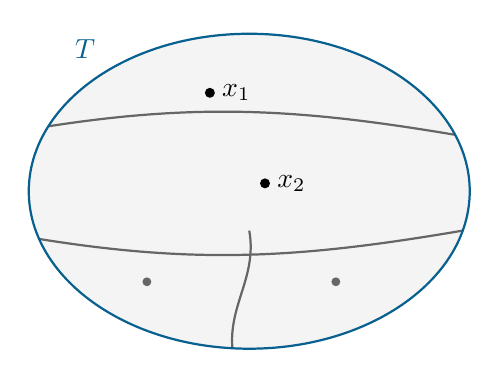
\begin{tikzpicture}
    % (1) Fill of T
    \fill[figLightGray!12] (0, 0) ellipse (2.8 and 2.0);

    % (2) Orbit boundaries clipped inside T
    \begin{scope}
        \clip (0, 0) ellipse (2.8 and 2.0);
        \draw[thick, figGray] (-3.0, 0.75) to[out=10, in=170] (3.0, 0.65);
        \draw[thick, figGray] (-3.0, -0.55) to[out=-10, in=190] (3.0, -0.45);
        \draw[thick, figGray] (0.0, -0.50) to[out=-80, in=100] (-0.2, -2.1);
    \end{scope}

    % (3) Outline of T
    \draw[thick, figBlue] (0, 0) ellipse (2.8 and 2.0);

    % (4) Orbit representatives
    \fill ( -0.5, 1.25) circle (1.8pt);
    \fill (  0.2, 0.10) circle (1.8pt);
    \fill[figGray] (-1.3, -1.15) circle (1.6pt);
    \fill[figGray] ( 1.1, -1.15) circle (1.6pt);

    % (5) Text last
    \node[anchor=south east, inner sep=0.15cm, figBlue] at (-1.80, 1.53) {$T$};
    \node[anchor=west, inner sep=0.15cm] at (-0.5, 1.25) {$x_1$};
    \node[anchor=west, inner sep=0.15cm] at (0.2, 0.10) {$x_2$};
\end{tikzpicture}
\end{center}

Summing the sizes of the disjoint orbits (as in Week 9, \cref{prop:orbit-decomposition}) and applying the finite Orbit-Stabilizer Theorem \eqref{eq:orb-stab-card-finite} to each orbit yields
\begin{align}
|T| = \binom{n}{p^k} &= \sum_{x_i \in \text{Orbits}} |\operatorname{Orb}(x_i)| \nonumber \\
&= \sum_{x_i} \frac{\left|\faktor{\mathbb{Z}}{p^k\mathbb{Z}}\right|}{|\operatorname{Stab}(x_i)|}. \label{eq:orbit-sum-stabilizer}
\end{align}
\end{content}

\begin{hidden}
% timestamp: 00:40:58
% topic: Orbit partition of T and Orbit-Stabilizer sum for \binom{n}{p^k}
% board_state: clm:binomial-nondivisibility, eq:card-t, eq:action-on-that, eq:induced-action-on-t, eq:orbit-sum-stabilizer
% next_goal: Analyze divisors of p^k, reduce modulo p to fixed points, and handle mid-lecture break
% open_loops: identify the fixed points of G on T to evaluate \binom{n}{p^k} mod p
\end{hidden}

\begin{speech}[00:40:58 - 00:41:53]
And the observation here is that the top is $p^k$ \inlinemetanote{draws an arrow from $|\faktor{\mathbb{Z}}{p^k\mathbb{Z}}|$ up-right to $p^k$}. And the stabilizer has to then divide $p^k$. So, this number here \inlinemetanote{circles $\frac{|\faktor{\mathbb{Z}}{p^k\mathbb{Z}}|}{|\operatorname{Stab}(x_i)|}$} is a divisor of $p^k$ \inlinemetanote{writes \qt{is a divisor of $p^k$}}, just because you take a number --- this is $p^k$ --- and you're quotienting $p^k$ by some integer, so the result here is a divisor of $p^k$.

And such divisors of $p^k$ are always divisible by $p$ \inlinemetanote{writes \qt{which is always div by $p$}}, except in one case. So, when is this not divisible by $p$? Yeah?
\end{speech}

\begin{speech}[00:41:53 - 00:42:32]
\inlinemetanote{faint, partly inaudible answer from a student} Yeah. If the stabilizer's the whole thing, then it's $1$. You know, $1$ is a divisor of $p^k$, but it's not divisible by $p$. So, it's always divisible by $p$ except when the stabilizer of $x$ is equal to the whole thing \inlinemetanote{writes \qt{except when $\operatorname{Stab}(x) = \faktor{\mathbb{Z}}{p^k\mathbb{Z}}$}}. Okay?

So, we get kind of a strange equation.
\end{speech}

\begin{content}[Divisibility of Orbit Sizes by \texorpdfstring{$p$}{p}]
In each summand $\frac{\left|\faktor{\mathbb{Z}}{p^k\mathbb{Z}}\right|}{|\operatorname{Stab}(x_i)|}$ of \eqref{eq:orbit-sum-stabilizer}, the numerator is $|\faktor{\mathbb{Z}}{p^k\mathbb{Z}}| = p^k$, and $|\operatorname{Stab}(x_i)|$ divides $p^k$ by Lagrange's theorem (\cref{thm:lagrange}). Therefore, every orbit size
\[
|\operatorname{Orb}(x_i)| = \frac{p^k}{|\operatorname{Stab}(x_i)|} \quad \text{is a divisor of } p^k.
\]
Since $p$ is prime, the positive divisors of $p^k$ are precisely $1, p, p^2, \dots, p^k$. Consequently, each orbit size is \emph{always divisible by $p$} except in the single case where the quotient equals $1$ --- namely, when $\operatorname{Stab}(x_i)$ is the entire group $G = \faktor{\mathbb{Z}}{p^k\mathbb{Z}}$:
\[
p \;\Big|\; \frac{p^k}{|\operatorname{Stab}(x_i)|} \qquad \text{except when } \operatorname{Stab}(x_i) = G \text{ (in which case } |\operatorname{Orb}(x_i)| = 1\text{)}.
\]
\end{content}

\begin{speech}[00:43:03 - 00:45:00]
We get this strange equation that says that the size of $T$, which I remind you is $n$ choose $p^k$, is equal to the number of fixed points --- I'll explain --- $\bmod\; p$ \inlinemetanote{writes \qt{$|T| = \text{\# Fixed point mod } p$} and \qt{$\binom{n}{p^k}$} below $|T|$}.

So, the fixed points here... this is $G$ acts on $T$ \inlinemetanote{writes \qt{$G \curvearrowright T$} and \qt{$= \faktor{\mathbb{Z}}{p^k\mathbb{Z}}$} vertically beneath $G$}, and a fixed point $x$ in $T$, by definition, is a point such that the stabilizer of $x$ is all of the $G$ here \inlinemetanote{writes: a fixed pt $x \in T \stackrel{\text{def}}{\iff} \operatorname{Stab}(x) = G$}. All right?

So, I'm using $G$, but $G$ is, if you remember, $\faktor{\mathbb{Z}}{p^k\mathbb{Z}}$. So, $G$ acts on our set $T$, and there's those points where the stabilizer is all of $G$, and they give us $1$'s in this equation \inlinemetanote{points at $\sum_{x_i} \frac{|\faktor{\mathbb{Z}}{p^k\mathbb{Z}}|}{|\operatorname{Stab}(x_i)|}$ on the upper board}. Because the stabilizer's all of it, so it's just $1$. Every one of those counts as $1$, and, you know, that's the number of fixed points \inlinemetanote{points at \qt{\# Fixed point}}. And then every other orbit, every other issue here \inlinemetanote{points at the remaining terms of the sum} is divisible by $p$. The fixed points are the only ones where it's not divisible by $p$, so they will be giving something with a $p$ in it. So, we get this equation.

And so, the final thing is: what are the fixed points of this $G = \mathbb{Z} \bmod p^k \mathbb{Z}$ action on $T$ \inlinemetanote{writes: What are Fixed points of $G = \faktor{\mathbb{Z}}{p^k\mathbb{Z}}$ action on $T$?}?

Okay, I'll explain this. \inlinemetanote{classroom bell chimes; video fades to black for the mid-lecture break}
\end{speech}

\begin{content}[Fixed-Point Congruence Modulo \texorpdfstring{$p$}{p}]
\begin{definition}[Fixed Point]\label[definition]{def:g-fixed-point}
Let $G = \faktor{\mathbb{Z}}{p^k\mathbb{Z}}$ act on $T$ ($G \curvearrowright T$). An element $x \in T$ is called a \newterm{fixed point} if its stabilizer is the entire group:
\[
x \in T \text{ is a fixed point} \stackrel{\text{def}}{\iff} \operatorname{Stab}(x) = G.
\]
\end{definition}

Separating the sum \eqref{eq:orbit-sum-stabilizer} into fixed points (each contributing $|\operatorname{Orb}(x_i)| = 1$) and all non-trivial orbits (each of size divisible by $p$) leaves the equation modulo $p$ (written informally with $=$ on the board: $|T| = \text{\# Fixed point mod } p$):
\begin{equation}\label{eq:fixed-pt-congruence}
|T| = \binom{n}{p^k} \equiv \#\text{Fixed points} \pmod{p}.
\end{equation}
Thus, to finish the proof, the remaining question is:
\[
\text{What are the fixed points of the } G = \faktor{\mathbb{Z}}{p^k\mathbb{Z}} \text{ action on } T\text{?}
\]
\end{content}

\begin{pause}[Mid-Lecture Break]
The classroom bell rings and the video fades out as the lecturer pauses before answering what the fixed points of the $\faktor{\mathbb{Z}}{p^k\mathbb{Z}}$-action on $T$ are. When the recording resumes after the break, the projection screen covers the upper board area, the lower chalkboard has been wiped clean, and students are returning to their seats.
\end{pause}

\subsection{Rebuilding the Proof After the Break}

\begin{speech}[00:45:02 - 00:47:01]
Okay, so, we start, and I'm going to start kind of again at the beginning of this argument, because there were a lot of questions and... you know, this argument is not logically complicated. The argument will turn out, when you understand it, to be logically simple, but the part that's complicated is the construction of all the group actions. It's a strange kind of argument because all the ideas are in the setup of the group actions. And so, you have to understand that, and the good news is I can explain it, and it's not that hard. You just have to, you know... yeah, so it's a weird kind of proof that way.

So, we're trying to prove this strange property that $n$ is equal to $p^k$ times $m$, where that's all of the $p$'s in $n$, and we want to prove that this $p$ does not divide \inlinemetanote{writes \qt{$n = p^k m$} and \qt{$p \nmid \binom{n}{p^k}$}}. That's our goal \inlinemetanote{writes \qt{Goal} and underlines $p \nmid \binom{n}{p^k}$ twice}.

And the strategy is, out of nowhere, to have this group $G$, $\mathbb{Z} \bmod p^k \mathbb{Z}$ \inlinemetanote{writes: $G = \faktor{\mathbb{Z}}{p^k\mathbb{Z}}$}. And I will in the argument just always call it $G$ instead of always writing this $p^k$. That was maybe part of the confusion.

So, that's the group, and then we want to construct --- again, this is where the idea in this proof is --- we need to construct an action onto a set. And you can imagine if we're going to use this Orbit-Stabilizer theorem at the end, we need to find a set that has order $n$ choose $p^k$. That's our goal. All right?

And the way that this went before --- the way the argument went --- is that the first thing I do is I construct this set $\widehat{T}$, and this set is just $G$ cross $1$ to $m$ \inlinemetanote{writes: $\widehat{T} = G \times \{1, \dots, m\}$}. And this set has order $n$, which is $p^k$ --- that's from this side --- times $m$ from that side \inlinemetanote{writes: $|\widehat{T}| = n = p^k \cdot m$}.

And this is of course not the set we're going to eventually want to study, because we need to have a set that has this $n$ choose $p^k$. But this set, it's good to maybe understand more carefully than I did, because I went a little bit fast on that.
\end{speech}

\begin{content}[Goal and Auxiliary Set \texorpdfstring{$\widehat{T}$}{T-hat} Restated]
Writing $n = p^k m$ (with $p \nmid m$), our goal is to prove
\[
p \nmid \binom{n}{p^k}.
\]
To keep notation clean, we fix the cyclic group
\[
G := \faktor{\mathbb{Z}}{p^k\mathbb{Z}}, \qquad |G| = p^k,
\]
and refer to it simply as $G$. As a first auxiliary step, we form the set
\[
\widehat{T} := G \times \{1, \dots, m\},
\]
which has cardinality
\[
|\widehat{T}| = n = p^k \cdot m.
\]
\end{content}

\begin{speech}[00:47:01 - 00:48:14]
So, it's incredibly important in this to understand the action $G$ cross $\widehat{T}$ to $\widehat{T}$, because that's the source of the action on the subsets \inlinemetanote{writes: $G \times \widehat{T} \to \widehat{T}$}. This is saying: if I have this element $g$ here, and this thing here is $(h, i)$, then this goes to $(gh, i)$, okay \inlinemetanote{writes: $g \times (h, i) \to (gh, i)$}?

In our case it's this group $\mathbb{Z} \bmod p^k$ in addition. So, all it's doing is acting on the first coordinate. So, I had written this before as: this $G$ is $\mathbb{Z} \bmod p^k \mathbb{Z}$, and this is cross $\mathbb{Z} \bmod p^k \mathbb{Z}$ cross $1$ to $m$ \inlinemetanote{writes: $\faktor{\mathbb{Z}}{p^k\mathbb{Z}} \times \left( \faktor{\mathbb{Z}}{p^k\mathbb{Z}} \times \{1, \dots, m\} \right)$}. And I wrote it as $\alpha$, and then I have to say what $(\beta, i)$ goes to, and this goes to $(\alpha + \beta, i)$ \inlinemetanote{writes: $\alpha \times (\beta, i) \longmapsto (\alpha + \beta, i)$}.

So, this action is not a very difficult one to think about: it's just the $G$-action on itself, and then it's that $G$-action on itself put together $m$ times. You know, that's all that's going on here.
\end{speech}

\begin{content}[The \texorpdfstring{$G$}{G}-Action on \texorpdfstring{$\widehat{T}$}{T-hat} in Multiplicative and Additive Notation]
The source of the entire construction is the action $G \times \widehat{T} \to \widehat{T}$ acting solely on the first coordinate by left translation:
\[
g, (h, i) \longmapsto (gh, i) \qquad \bigl(g, h \in G,\; i \in \{1, \dots, m\}\bigr).
\]
Writing $G = \faktor{\mathbb{Z}}{p^k\mathbb{Z}}$ explicitly in additive notation, this is the map
\begin{align*}
\faktor{\mathbb{Z}}{p^k\mathbb{Z}} \times \left( \faktor{\mathbb{Z}}{p^k\mathbb{Z}} \times \{1, \dots, m\} \right) &\longrightarrow \faktor{\mathbb{Z}}{p^k\mathbb{Z}} \times \{1, \dots, m\}, \\
\alpha, (\beta, i) &\longmapsto (\alpha + \beta, i).
\end{align*}
Conceptually, this is simply the left translation action of $G$ on itself, replicated in parallel across $m$ independent copies of $G$.
\end{content}

\begin{speech}[00:48:14 - 00:49:30]
So, it's the first thing to understand, that there is this set $\widehat{T}$ \inlinemetanote{writes $\widehat{T}$ and draws a large loop}. And you can imagine this set $\widehat{T}$, if you want to picture it, is that there's one copy of $\mathbb{Z} \bmod p \mathbb{Z}$ (i.e., $\faktor{\mathbb{Z}}{p^k\mathbb{Z}}$)... $p\mathbb{Z}$ to the $k$ here, and there's another copy, another copy, there's another copy, there's another copy \inlinemetanote{draws five vertical columns of dots inside $\widehat{T}$}. The number of copies is $m$ \inlinemetanote{draws a brace above the columns labeled $m$}. You just put it in $m$ times, one for every index here \inlinemetanote{points at $\{1, \dots, m\}$}. Right? And then its action is just spinning the way that the group acts on itself, on each one of these \inlinemetanote{gestures rotating along one column}. Okay?

So, is that clear how it's going on here? This is the first idea, is to make this set. And it's not clear why you do this --- of course in this kind of argument, the reasons all come at the end, in the punchline --- but we make this set. And this is not the set which we apply the Orbit-Stabilizer theorem to. It's an auxiliary step, it's a first step.

But is it clear what this thing is? And what's very important is its order is $n$ \inlinemetanote{writes \qt{$= n$} next to $\widehat{T}$}. And as I said, if you want to picture it, you just picture it like that \inlinemetanote{points at the $m$-column picture of $\widehat{T}$}: there's my group, and I just put it together --- just as a set --- put it together $m$ times. This is $m$ of them. Okay?
\end{speech}

\begin{content}[Visualizing \texorpdfstring{$\widehat{T}$}{T-hat} as \texorpdfstring{$m$}{m} Parallel Copies of \texorpdfstring{$G$}{G}]
We can picture $\widehat{T}$ (of total size $|\widehat{T}| = n$) as $m$ disjoint columns sitting side by side, each column being one copy of $G = \faktor{\mathbb{Z}}{p^k\mathbb{Z}}$ on which $G$ acts independently by cyclic translation:

\definecolor{figBlue}{HTML}{07608F} % RGB (7, 96, 143): petrol blue (MidnightBlue)
\definecolor{figGray}{HTML}{666666} % RGB (102, 102, 102): dark gray (gray!80!black)
\definecolor{figLightGray}{HTML}{A6A6A6} % RGB (166, 166, 166): light gray (gray!70)
\begin{hidden}
- Canvas: no scale, cm; ellipse \widehat{T} centered at (0, 0) with radii 3.6 and 2.5; note outside right at (4.1, 0); picture spans x in [-3.6, 6.8], y in [-2.6, 2.9]
- Order: (1) light fill of \widehat{T}; (2) light rounded box highlighting the rightmost copy of G; (3) outline of \widehat{T}; (4) brace above the 5 columns; (5) 5 columns of 4 dots each; (6) pointer arrow to rightmost copy; (7) all text last
- Coordinates:
  \widehat{T}: ellipse at (0, 0), radii 3.6 and 2.5.
  5 columns at x = -2.0, -1.0, 0.0, 1.0, 2.0 (1.0 cm horizontal spacing); 4 dots per column at y = 0.9, 0.3, -0.3, -0.9 (0.6 cm vertical spacing).
  At x = +-2.0, ellipse y = +-2.5 * sqrt(1 - (2.0/3.6)^2) = +-2.08 (dots at y = +-0.9 stay 1.18 cm inside!).
  Rightmost copy box: rounded rectangle (1.65, -1.15) to (2.35, 1.15).
  Curly brace above columns: from (-2.1, 1.30) to (2.1, 1.30), amplitude 6pt (top ~1.51; at x = +-2.1, ellipse y = +-2.03 > 1.51).
  Pointer from outside note: (4.1, 0) to (2.35, 0) (crosses right edge (3.6, 0) cleanly between rows y = +-0.3).
- Labels (attached, inner sep=0.15cm):
  "\widehat{T}" at (130:3.6 and 2.5) = (-2.31, 1.92) with anchor=south east.
  "|\widehat{T}| = n" at (50:3.6 and 2.5) = (2.31, 1.92) with anchor=south west.
  "m" at (0, 1.50) with anchor=south (top around 1.95, 0.55 cm below ellipse top 2.5).
  "one copy of $G$" at (4.1, 0) with anchor=west.
- Collisions: "m" sits 0.55 cm below the top of \widehat{T} and 0.20 cm above the brace; outer labels sit outside \widehat{T} in free directions; outside note lies right of (4.1, 0).
\end{hidden}
\begin{center}
\begin{tikzpicture}[>=Stealth]
    % (1), (2) Background fill and highlight of one copy of G
    \fill[figLightGray!12] (0, 0) ellipse (3.6 and 2.5);
    \filldraw[fill=figBlue!10, draw=figBlue!60, rounded corners=4pt] (1.65, -1.15) rectangle (2.35, 1.15);

    % (3) Outline of \widehat{T}
    \draw[thick, figGray] (0, 0) ellipse (3.6 and 2.5);

    % (4) Curly brace over the m columns
    \draw[thick, decorate, decoration={brace, amplitude=6pt}] (-2.1, 1.30) -- (2.1, 1.30);

    % (5) Columns representing copies of G = Z/p^kZ
    \foreach \colx in {-2.0, -1.0, 0.0, 1.0, 2.0} {
        \foreach \rowy in {0.9, 0.3, -0.3, -0.9} {
            \fill[figBlue] (\colx, \rowy) circle (1.8pt);
        }
    }

    % (6) Pointer from outside note
    \draw[->, thin, figBlue] (4.1, 0) -- (2.35, 0);

    % (7) Text last
    \node[anchor=south east, inner sep=0.15cm, figGray] at (-2.31, 1.92) {$\widehat{T}$};
    \node[anchor=south west, inner sep=0.15cm, figGray] at (2.31, 1.92) {$|\widehat{T}| = n$};
    \node[anchor=south, inner sep=0.15cm] at (0, 1.50) {$m$};
    \node[anchor=west, inner sep=0.15cm, figBlue] at (4.1, 0) {one copy of $G$};
\end{tikzpicture}
\end{center}
\end{content}

\begin{hidden}
% timestamp: 00:49:30
% topic: Rebuilt auxiliary set \widehat{T} as m columns of G = Z/p^kZ
% board_state: clm:binomial-nondivisibility, eq:fixed-pt-congruence
% next_goal: Redraw the induced action of G on the subset space T and partition T into orbits
% open_loops: answer the fixed-point question to compute \binom{n}{p^k} mod p
\end{hidden}

\begin{speech}[00:49:31 - 00:51:04]
So, then the action for this proof doesn't occur on this set. It acts on this set $T$, which is the set of $p^k$-element subsets of $\widehat{T}$ \inlinemetanote{writes: $T = \{ \text{set of } p^k\text{-elmt subsets of } \widehat{T} \}$}.

All right, so, what is a $p^k$-element subset? It means I go here and I pick $p^k$ elements --- so I could pick them like this \inlinemetanote{draws a red loop enclosing elements across columns inside $\widehat{T}$}, you know, I don't know, however --- you pick some subset of $p^k$ elements. All right?

And the claim is that there's an action here: $G \times T$ goes to $T$ \inlinemetanote{writes: $G \times T \to T$ action}. And the action is just: if you give me a $p^k$-element subset --- that's this thing in red \inlinemetanote{points at the red loop inside $\widehat{T}$} --- I need to get a new $p^k$-element subset, that's what action is. And I just take my element of $G$ and just move each element, and that gives me a new $p^k$-element subset. So, is that clear?

And then you have to check it's an action --- that's always nothing to check --- so, if you understand the setup, we have this group $G$, $\faktor{\mathbb{Z}}{p^k\mathbb{Z}}$, and it acts on this set $T$ goes to $T$ \inlinemetanote{writes: $\faktor{\mathbb{Z}}{p^k\mathbb{Z}} \times T \to T$}. All right? And it's impossible to understand this proof unless you understand this picture, what's happening there, because that's where all the ideas in the proof are pretty much, setting this up.
\end{speech}

\begin{content}[The Subset Space \texorpdfstring{$T$}{T} and the Induced \texorpdfstring{$G$}{G}-Action]
The actual action used in the proof takes place on
\[
T = \{ \text{set of } p^k\text{-element subsets of } \widehat{T} \}.
\]
Each element $S \in T$ is a subset of $p^k$ points chosen inside the $m$ copies of $G$ making up $\widehat{T}$ (shown in red below):

\definecolor{chalkRed}{HTML}{D2645A} % RGB (210, 100, 90): red chalk read from the frame
\definecolor{figBlue}{HTML}{07608F} % RGB (7, 96, 143): petrol blue (MidnightBlue)
\definecolor{figGray}{HTML}{666666} % RGB (102, 102, 102): dark gray (gray!80!black)
\definecolor{figLightGray}{HTML}{A6A6A6} % RGB (166, 166, 166): light gray (gray!70)
\begin{hidden}
- Canvas: no scale, cm; ellipse \widehat{T} centered at (0, 0) with radii 3.6 and 2.5; note below at (-0.5, -2.9); picture spans x in [-3.6, 4.2], y in [-3.5, 2.9]
- Order: (1) light fill of \widehat{T}; (2) red subset fill inside \widehat{T}; (3) outline of \widehat{T} and red subset outline; (4) curly brace above columns; (5) dots (4 red inside subset, rest blue); (6) pointer from below note; (7) all text last
- Coordinates:
  \widehat{T}: ellipse at (0, 0), radii 3.6 and 2.5.
  Columns: x = -2.0, -1.0, 0.0, 1.0, 2.0; rows: y = 0.9, 0.3, -0.3, -0.9.
  Red subset S: ellipse at (-0.50, 0.0), radii 0.85 and 0.55 (x in [-1.35, 0.35], y in [-0.55, 0.55]).
  Check membership:
    (-1.0, +-0.3) and (0.0, +-0.3): ((-0.5)/0.85)^2 + (0.3/0.55)^2 = 0.346 + 0.298 = 0.644 < 1 (strictly inside).
    All other dots are at least 0.35 cm outside S (e.g., (-2.0, 0.3) is 0.65 left, (-1.0, 0.9) is 0.35 above).
  Pointer from below note: from (-0.5, -2.9) straight up to (-0.5, -0.55), running right down the 1.0 cm corridor between columns x = -1.0 and x = 0.0.
- Labels (attached, inner sep=0.15cm):
  "\widehat{T}" at (130:3.6 and 2.5) = (-2.31, 1.92) anchor=south east;
  "|\widehat{T}| = n" at (50:3.6 and 2.5) = (2.31, 1.92) anchor=south west;
  "m" at (0, 1.50) anchor=south;
  "subset $S \in T$ ($|S| = p^k$)" at (-0.5, -2.9) anchor=north (below \widehat{T}, clear of y = -2.5).
- Collisions: vertical pointer at x = -0.5 passes midway between columns 2 and 3 (0.5 cm from all dots); outside note sits 0.4 cm below the bottom of \widehat{T}.
\end{hidden}
\begin{center}
\begin{tikzpicture}[>=Stealth]
    % (1), (2) Fills
    \fill[figLightGray!12] (0, 0) ellipse (3.6 and 2.5);
    \fill[chalkRed!12] (-0.50, 0.0) ellipse (0.85 and 0.55);

    % (3) Outlines
    \draw[thick, figGray] (0, 0) ellipse (3.6 and 2.5);
    \draw[thick, chalkRed!80!black] (-0.50, 0.0) ellipse (0.85 and 0.55);

    % (4) Curly brace over the m columns
    \draw[thick, decorate, decoration={brace, amplitude=6pt}] (-2.1, 1.30) -- (2.1, 1.30);

    % (5) Column dots (red inside S, blue outside)
    \foreach \colx in {-2.0, 1.0, 2.0} {
        \foreach \rowy in {0.9, 0.3, -0.3, -0.9} {
            \fill[figBlue] (\colx, \rowy) circle (1.8pt);
        }
    }
    \foreach \colx in {-1.0, 0.0} {
        \foreach \rowy in {0.9, -0.9} {
            \fill[figBlue] (\colx, \rowy) circle (1.8pt);
        }
        \foreach \rowy in {0.3, -0.3} {
            \fill[chalkRed!80!black] (\colx, \rowy) circle (1.8pt);
        }
    }

    % (6) Pointer from outside note
    \draw[->, thin, chalkRed!80!black] (-0.5, -2.9) -- (-0.5, -0.55);

    % (7) Text last
    \node[anchor=south east, inner sep=0.15cm, figGray] at (-2.31, 1.92) {$\widehat{T}$};
    \node[anchor=south west, inner sep=0.15cm, figGray] at (2.31, 1.92) {$|\widehat{T}| = n$};
    \node[anchor=south, inner sep=0.15cm] at (0, 1.50) {$m$};
    \node[anchor=north, inner sep=0.15cm, chalkRed!80!black] at (-0.5, -2.9) {subset $S \in T$ ($|S| = p^k$)};
\end{tikzpicture}
\end{center}

Acting on $S \in T$ by an element $g \in G = \faktor{\mathbb{Z}}{p^k\mathbb{Z}}$ moves every element of $S$ within its column, yielding a new $p^k$-element subset and thus defining the group action
\[
G \times T \longrightarrow T \qquad \left(\text{i.e., } \faktor{\mathbb{Z}}{p^k\mathbb{Z}} \times T \to T\right).
\]
\end{content}

\begin{speech}[00:51:05 - 00:51:20]
Okay, so, then, how to use this group action is we use the way we know how to count sets by their orbits. So, here's my picture of $T$ \inlinemetanote{draws a loop labeled $T$ on the lower-left board}. And the elements of $T$ are these red things \inlinemetanote{points at the red subset inside $\widehat{T}$}. Yeah?
\end{speech}

\begin{student}[Student Question]
How do we know a $p^k$-element subset necessarily maps to a $p^k$-element subset?
\end{student}

\begin{speech}[00:51:26 - 00:51:46]
Good question. And how do you know that? \inlinemetanote{student pauses to think} It's because every element of $G$ acts by bijection in a group action.

If you have a group action, $G$ spins your $T$ (i.e., $\widehat{T}$) or whatever subset around, but it's always a bijection. And the reason it's always a bijection is the group has an inverse element, and when you apply it, you get the identity.
\end{speech}

\begin{student}[Student Remark]
Okay, thank you.
\end{student}

\begin{speech}[00:51:48 - 00:53:29]
All right. No, that's a good question. He's worried that if I take this $p^k$-element subset and I apply the elements of $G$, some points could, I don't know, crash together or something bad could happen. It can't happen. When the group acts on this, it's a bijection.

Okay, so, here's $T$, that's our set of the red subsets. Maybe in an impromptu pedagogical move, I will put the points here to be red \inlinemetanote{draws four red dots inside $T$}. So, each red point corresponds to the subset \inlinemetanote{points at the red subset inside $\widehat{T}$}. Okay? And the white points \inlinemetanote{points at the white dots in $\widehat{T}$} are the actual elements of $\widehat{T}$.

And now we know that $T$ --- it's a finite set, it has cardinality $n$, $p^k$ \inlinemetanote{writes: $|T| = \binom{n}{p^k}$} --- and it has the $G$-action, so I can divide it up into its orbits \inlinemetanote{draws curved partition lines inside $T$}. All right? So, that's its division into its orbits, and I pick one element $x_i$ in every orbit so I can talk about it \inlinemetanote{marks dots labeled $x_1, x_2$ in two of the orbits}. It has these orbits, finitely many orbits. For each orbit I pick one element.

And then I write down my equation, which says that the size of $T$ is equal to the sum over all of these $x_i$, and then the size of the orbit \inlinemetanote{writes \qt{$|T| = \sum_{x_i} |\operatorname{Orb}(x_i)|$} and writes \qt{$\binom{n}{p^k}$} underneath $|T|$}. So, this is an entirely uncontroversial statement: I've just taken this $P$ (i.e., $T$) and I've cut it up into the orbits. And now I want to apply the Orbit-Stabilizer theorem for each one of these --- remember, this is $n$, $p^k$ --- so to each one of these I apply the Orbit-Stabilizer theorem.
\end{speech}

\begin{content}[Counting \texorpdfstring{$T$}{T} by Its Orbits]
We now visualize $T$ itself as a finite set of cardinality $|T| = \binom{n}{p^k}$ whose points (drawn in red) correspond to the $p^k$-element subsets of $\widehat{T}$, partitioned into finitely many disjoint $G$-orbits with chosen representatives $x_i$:

\definecolor{chalkRed}{HTML}{D2645A} % RGB (210, 100, 90): red chalk read from the frame
\definecolor{figBlue}{HTML}{07608F} % RGB (7, 96, 143): petrol blue (MidnightBlue)
\definecolor{figGray}{HTML}{666666} % RGB (102, 102, 102): dark gray (gray!80!black)
\definecolor{figLightGray}{HTML}{A6A6A6} % RGB (166, 166, 166): light gray (gray!70)
\begin{hidden}
- Canvas: no scale, cm; ellipse T centered at (0, 0) with radii 2.8 and 2.0; picture spans x in [-3.1, 3.0], y in [-2.1, 2.4]
- Order: (1) light fill of T; (2) orbit dividers clipped inside T; (3) outline of T; (4) red subset dots and representative dots; (5) all text last
- Coordinates:
  T: ellipse at (0, 0), radii 2.8 and 2.0.
  Clipped dividers:
    (-3.0, 0.75) to[out=10, in=170] (3.0, 0.65);
    (-3.0, -0.55) to[out=-10, in=190] (3.0, -0.45);
    (0.0, -0.50) to[out=-80, in=100] (-0.2, -2.1).
  Red dots (subsets in T): (-1.2, 1.15), (1.2, 1.15), (-0.9, 0.15), (1.2, -0.05), (-1.55, -1.15), (1.0, -1.25).
  Chosen representatives: x_1 at (-0.1, 1.25) (between (-1.2, 1.15) and (1.2, 1.15)); x_2 at (0.1, 0.15) (between (-0.9, 0.15) and (1.2, -0.05)).
- Labels (attached, inner sep=0.15cm):
  "T" at (130:2.8 and 2.0) = (-1.80, 1.53) with anchor=south east.
  "x_1" at (-0.1, 1.25) with anchor=west (ends around x = 0.45, leaving 0.75 cm before (1.2, 1.15)).
  "x_2" at (0.1, 0.15) with anchor=west (ends around x = 0.65, leaving 0.55 cm before (1.2, -0.05)).
- Collisions: x_1 and x_2 lie cleanly inside their orbits, well clear of all red dots and dividers.
\end{hidden}
\begin{center}
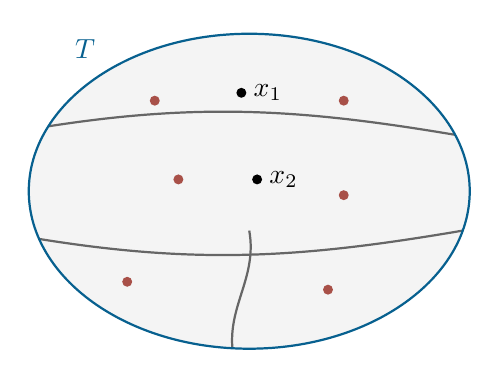
\begin{tikzpicture}
    % (1) Fill of T
    \fill[figLightGray!12] (0, 0) ellipse (2.8 and 2.0);

    % (2) Orbit dividers clipped inside T
    \begin{scope}
        \clip (0, 0) ellipse (2.8 and 2.0);
        \draw[thick, figGray] (-3.0, 0.75) to[out=10, in=170] (3.0, 0.65);
        \draw[thick, figGray] (-3.0, -0.55) to[out=-10, in=190] (3.0, -0.45);
        \draw[thick, figGray] (0.0, -0.50) to[out=-80, in=100] (-0.2, -2.1);
    \end{scope}

    % (3) Outline of T
    \draw[thick, figBlue] (0, 0) ellipse (2.8 and 2.0);

    % (4) Points in T (red dots = subsets of \widehat{T}) and representatives x_1, x_2
    \fill[chalkRed!80!black] (-1.2, 1.15) circle (1.8pt) (1.2, 1.15) circle (1.8pt)
                             (-0.9, 0.15) circle (1.8pt) (1.2, -0.05) circle (1.8pt)
                             (-1.55, -1.15) circle (1.8pt) (1.0, -1.25) circle (1.8pt);
    \fill (-0.1, 1.25) circle (1.8pt);
    \fill ( 0.1, 0.15) circle (1.8pt);

    % (5) Text last
    \node[anchor=south east, inner sep=0.15cm, figBlue] at (-1.80, 1.53) {$T$};
    \node[anchor=west, inner sep=0.15cm] at (-0.1, 1.25) {$x_1$};
    \node[anchor=west, inner sep=0.15cm] at (0.1, 0.15) {$x_2$};
\end{tikzpicture}
\end{center}

Summing over the orbit representatives $x_i$ yields
\[
|T| = \binom{n}{p^k} = \sum_{x_i} |\operatorname{Orb}(x_i)|.
\]

\begin{steps}[Why Acting by \texorpdfstring{$g \in G$}{g in G} Preserves Subset Cardinality]
Because $G \times \widehat{T} \to \widehat{T}$ is a group action, every $g \in G$ acts on $\widehat{T}$ by a \emph{bijection} (Week 9, \cref{cor:action-bijection}): its inverse map is the action of $g^{-1} \in G$ (since $g^{-1} \cdot (g \cdot y) = (g^{-1} g) \cdot y = e \cdot y = y$ and $g \cdot (g^{-1} \cdot y) = y$). Therefore, no two distinct elements of a subset $S \subset \widehat{T}$ can collide under $g$, so $|g \cdot S| = |S| = p^k$ always holds.
\end{steps}
\end{content}

\begin{hidden}
% timestamp: 00:53:29
% topic: Redrawn T partitioned into orbits with red points representing p^k-element subsets
% board_state: clm:binomial-nondivisibility, def:g-fixed-point, eq:fixed-pt-congruence
% next_goal: Reduce goal modulo p, distinguish 1-point orbits from larger orbits of size p^\ell
% open_loops: prove that non-trivial orbits have size p^\ell and count fixed points
\end{hidden}

\begin{speech}[00:53:29 - 00:55:07]
And at the very beginning, what we're interested in... I just remind you: our goal is $p$ does not divide the order here \inlinemetanote{writes \qt{Goal:} and \qt{$p \nmid \binom{n}{p^k}$}}. Okay? This is equivalent to saying that this binomial is not congruent to $0 \bmod p$. That's what we're trying to show \inlinemetanote{writes: $\iff \binom{n}{p^k} \neq 0 \bmod p$}. Okay?

So, everything is really about this fellow $\bmod\; p$ \inlinemetanote{points at $|T| = \sum_{x_i} |\operatorname{Orb}(x_i)|$}. We're interested in this fellow $\bmod\; p$. So, with that in mind, we look at this orbit.

This orbit of $x_i$ \inlinemetanote{writes: $\operatorname{Orb}(x_i)$}, it could be $1$ point \inlinemetanote{writes: $1\text{ pt}$}. That's possible, meaning that this $x_i$ is all by itself. That's the whole orbit. \inlinemetanote{circles a lone red dot inside $T$ and writes $x_{17}$ beside it} $x_{17}$, here he is, he's all by himself. Right? That could happen.

In which case, if it's $1$ point, then this $\operatorname{Orb}(x_i)$ counts as $1$ here in this sum \inlinemetanote{writes: $\longrightarrow |\operatorname{Orb}(x_i)| = 1$}. And this is by definition --- there's a definition which may be confusing in this part --- $x_i$ here is a \newterm{$G$-fixed point}. That's a definition \inlinemetanote{writes: $(x_i \text{ is } G\text{-fixed pt})$}. If you have an element in a $G$-action that doesn't go anywhere, it's called $G$-fixed for the reason that it doesn't go anywhere: the orbit is just itself. $G$ doesn't move it anywhere, it's called $G$-fixed.

So, in this thing, $x_i$ could be $1$ point --- the orbit could just consist of $1$ point --- and then it contributes $1$ here, clearly, right?
\end{speech}

\begin{content}[Goal Modulo \texorpdfstring{$p$}{p} and Singleton Orbits]
Recall our objective:
\[
\text{Goal:} \qquad p \nmid \binom{n}{p^k} \iff \binom{n}{p^k} \not\equiv 0 \pmod{p}.
\]
Because we only need $\binom{n}{p^k}$ modulo $p$, we examine the possible sizes of an orbit $\operatorname{Orb}(x_i)$. The first possibility is a $1$-point orbit ($1\text{ pt}$), such as a lone element $x_{17}$ sitting by itself in $T$:

\definecolor{chalkRed}{HTML}{D2645A} % RGB (210, 100, 90): red chalk read from the frame
\definecolor{figBlue}{HTML}{07608F} % RGB (7, 96, 143): petrol blue (MidnightBlue)
\definecolor{figGray}{HTML}{666666} % RGB (102, 102, 102): dark gray (gray!80!black)
\definecolor{figLightGray}{HTML}{A6A6A6} % RGB (166, 166, 166): light gray (gray!70)
\begin{hidden}
- Canvas: no scale, cm; ellipse T centered at (0, 0) with radii 2.8 and 2.0; picture spans x in [-3.1, 3.0], y in [-2.1, 2.4]
- Order: (1) light fill of T and of singleton circle around x_{17}; (2) orbit dividers clipped inside T; (3) outline of T and singleton circle; (4) red dots and representative dots; (5) all text last
- Coordinates:
  T: ellipse at (0, 0), radii 2.8 and 2.0.
  Clipped dividers: as before.
  Singleton orbit x_{17}: lone red dot at (-1.55, -1.15) enclosed by a circle of radius 0.32 (x in [-1.87, -1.23]).
  Vertical divider at y = -1.15 sits near x = -0.08, leaving 1.15 cm to the right.
- Labels (attached, inner sep=0.15cm):
  "T" at (-1.80, 1.53) anchor=south east; "x_1" at (-0.15, 1.30) anchor=west; "x_2" at (0.05, 0.15) anchor=west;
  "x_{17}" at (-1.23, -1.15) anchor=west (ends near x = -0.55, leaving >= 0.45 cm before the vertical divider).
- Collisions: x_{17} lies strictly inside the lower-left orbit, clear of its circle and the vertical divider.
\end{hidden}
\begin{center}
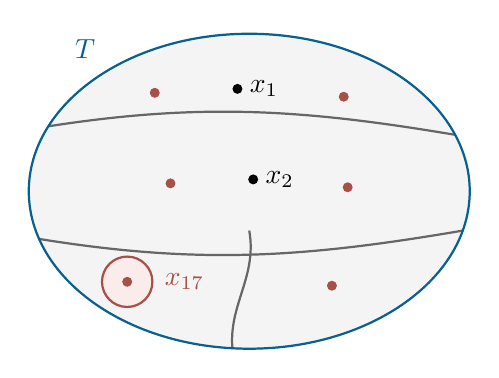
\begin{tikzpicture}
    % (1) Fills
    \fill[figLightGray!12] (0, 0) ellipse (2.8 and 2.0);
    \fill[chalkRed!12] (-1.55, -1.15) circle (0.32);

    % (2) Orbit dividers clipped inside T
    \begin{scope}
        \clip (0, 0) ellipse (2.8 and 2.0);
        \draw[thick, figGray] (-3.0, 0.75) to[out=10, in=170] (3.0, 0.65);
        \draw[thick, figGray] (-3.0, -0.55) to[out=-10, in=190] (3.0, -0.45);
        \draw[thick, figGray] (0.0, -0.50) to[out=-80, in=100] (-0.2, -2.1);
    \end{scope}

    % (3) Outlines of T and singleton orbit
    \draw[thick, figBlue] (0, 0) ellipse (2.8 and 2.0);
    \draw[thick, chalkRed!80!black] (-1.55, -1.15) circle (0.32);

    % (4) Points
    \fill[chalkRed!80!black] (-1.2, 1.25) circle (1.8pt) (1.2, 1.20) circle (1.8pt)
                             (-1.0, 0.10) circle (1.8pt) (1.25, 0.05) circle (1.8pt)
                             (-1.55, -1.15) circle (1.8pt) (1.05, -1.20) circle (1.8pt);
    \fill (-0.15, 1.30) circle (1.8pt);
    \fill ( 0.05, 0.15) circle (1.8pt);

    % (5) Text last
    \node[anchor=south east, inner sep=0.15cm, figBlue] at (-1.80, 1.53) {$T$};
    \node[anchor=west, inner sep=0.15cm] at (-0.15, 1.30) {$x_1$};
    \node[anchor=west, inner sep=0.15cm] at (0.05, 0.15) {$x_2$};
    \node[anchor=west, inner sep=0.15cm, chalkRed!80!black] at (-1.23, -1.15) {$x_{17}$};
\end{tikzpicture}
\end{center}

For $\operatorname{Orb}(x_i)$, the first case is:
\[
1\text{ pt} \longrightarrow |\operatorname{Orb}(x_i)| = 1 \qquad (x_i \text{ is } G\text{-fixed pt}).
\]
\begin{definition}[\texorpdfstring{$G$}{G}-Fixed Point]\label[definition]{def:g-fixed-pt-singleton}
An element $x_i \in T$ whose orbit consists only of itself ($|\operatorname{Orb}(x_i)| = 1$, i.e., $G$ does not move $x_i$ anywhere) is called a \newterm{$G$-fixed point}. Each $G$-fixed point contributes $1$ to $\sum_{x_i} |\operatorname{Orb}(x_i)|$.
\end{definition}
\end{content}

\begin{speech}[00:55:07 - 00:56:59]
Or it could be more points \inlinemetanote{draws an arrow down from $\operatorname{Orb}(x_i)$ and writes: more pts}. It's at least $1$ point because it has $x_i$ in it. And the claim here, if it's more points, the number of points has to be $p$ to the $\ell$ with $\ell$ positive \inlinemetanote{writes: $\longrightarrow \#\text{ pts have } p^{\ell > 0}$}. In other words, the size of the orbit is equal to $p$ to the $\ell$, where $\ell$ is positive \inlinemetanote{writes: $|\operatorname{Orb}(x_i)| = p^{\ell > 0}$}.

And the reason is that the size of this orbit, by the Orbit-Stabilizer theorem, is equal to the size of $G$ divided by the size of the stabilizer \inlinemetanote{writes: $\operatorname{Orb}(x_i) = \frac{|\faktor{\mathbb{Z}}{p^k\mathbb{Z}}|}{|\operatorname{Stab}(x_i)|}$, without bars on the left}. That's the Orbit-Stabilizer theorem. The guy on top here is $p$ to the $k$ \inlinemetanote{writes \qt{$\leftarrow p^k$} next to the numerator}. And if you take $p$ to the $k$ and you divide something to get a number, you could get $1$, that's if the stabilizer's the whole thing --- that's this case \inlinemetanote{points at the $1\text{ pt}$ branch}. But if you don't get $1$, you get a power of $p$, that's with $p$ to the $\ell$ with $\ell$ greater than $0$. Is that clear?

So, here, since the top is $p$ to the $k$, the result is either $1$ or $p$ to the $\ell$ with $\ell$ positive, and the $1$ was already this case, so it's not this one \inlinemetanote{writes \qt{so result is either $1$ or $p^{\ell > 0}$} and crosses out $1$}. Okay?

So, you happy with that logic? It's because this group has been cunningly chosen to have order a power of $p$, and this Orbit-Stabilizer theorem has to do with divisors of the size of that group, and $p$ to the $k$ has very few divisors. It's part of the cunningness of the setup here.

Then you come to the last equation I wrote.
\end{speech}

\begin{content}[Orbits With More Than One Point Have Size \texorpdfstring{$p^\ell$}{p\textasciicircum l}]
\begin{claim}[Cardinality of Non-Singleton Orbits]\label[claim]{clm:nontrivial-orbit-size}
If $\operatorname{Orb}(x_i)$ has more points ($\text{more pts}$, i.e., $|\operatorname{Orb}(x_i)| > 1$), then it has to have $p^\ell$ points with $\ell > 0$:
\[
|\operatorname{Orb}(x_i)| = p^\ell \qquad (\ell \ge 1).
\]
\end{claim}

\begin{proof}[Proof of \cref{clm:nontrivial-orbit-size}]
By the finite Orbit-Stabilizer Theorem \eqref{eq:orb-stab-card-finite},
\[
|\operatorname{Orb}(x_i)| = \frac{|G|}{|\operatorname{Stab}(x_i)|}.
\]
Since $|G| = \left|\faktor{\mathbb{Z}}{p^k\mathbb{Z}}\right| = p^k$, the quotient $\frac{p^k}{|\operatorname{Stab}(x_i)|}$ must be a positive divisor of $p^k$. Because $p$ is prime, its positive divisors are $1, p, p^2, \dots, p^k$; thus, the result is either $1$ or $p^\ell$ with $\ell > 0$. Since the case $|\operatorname{Orb}(x_i)| = 1$ (where $\operatorname{Stab}(x_i) = G$) was already separated out as the $1$-point fixed-point case, any orbit with more than one point must have cardinality $|\operatorname{Orb}(x_i)| = p^\ell$ for some $\ell > 0$.
\end{proof}
\end{content}

\begin{hidden}
% timestamp: 00:56:59
% topic: Completed orbit-size classification (1 vs. p^\ell) in the proof of p \nmid \binom{n}{p^k}
% board_state: clm:binomial-nondivisibility, def:g-fixed-pt-singleton, clm:nontrivial-orbit-size
% next_goal: Reduce |T| mod p to #fixed pts and determine the fixed points of G on T
% open_loops: identify the fixed points of G on T
\end{hidden}

\begin{speech}[00:57:08 - 00:58:20]
So, was this a good idea to have the red points? Maybe I keep it.

Actually, normally people... when I taught before, which I said I left the... I know people complain about my improvisational style of lecturing, but somehow this year I haven't really received too many complaints, so I don't know what the... There have been some complaints, not... yeah \inlinemetanote{inaudible question from a student}?

Because it's already there, it's in that case \inlinemetanote{points at the $1\text{ pt}$ branch on the upper board}. If you're in this branch, it has more than, you know, this \qt{more points}, not one point \inlinemetanote{points at the \qt{more pts} branch}. So, the one is one point, and the other is more than... maybe I could put \qt{more than one} \inlinemetanote{gestures at \qt{more pts}}. \inlinemetanote{inaudible follow-up from the student} Well, it's not a possibility when you're in the \qt{more points}. That's already been taken care of.

Okay, so, let's see if I can finish here.
\end{speech}

\subsubsection{Reduction to Fixed Points Modulo \texorpdfstring{$p$}{p}}

\begin{speech}[00:58:20 - 00:59:55]
So, if you rewrite this equation here \inlinemetanote{points at $|T| = \sum_{x_i} |\operatorname{Orb}(x_i)|$ on the upper board}, we get this equation that $n$ choose $p$ to the $k$, which is what we're interested in, is equal to the size of $T$, and this is equal to the number of fixed points $\bmod\; p$ \inlinemetanote{writes: $\binom{n}{p^k} = |T| = \#\text{fixed pts} \bmod p$}.

Why is that? Because I said, if you have a fixed point, it contributes $1$ \inlinemetanote{points at $|\operatorname{Orb}(x_i)| = 1$}. That's why we have the number of fixed points: each fixed point contributes $1$. Anything that's not a fixed point, it's in this \qt{more points}, and those orbits are all divisible by $p$ \inlinemetanote{points at $|\operatorname{Orb}(x_i)| = p^\ell$}. So, if I take $\bmod\; p$, they just go away. Okay? Are you happy with that? I just look at every one of these: this orbit is either $1$, then it contributes the fixed point, or this orbit is divisible by $p$, so it's $0 \bmod p$, so it contributes $0$ in this equation.

Okay, so, this is really good news for us, because the whole goal was to prove --- or \qt{is}, maybe \qt{is} is better tense --- is to prove this $n$, $p$ $k$ (i.e., $\binom{n}{p^k}$) is not equal to $0 \bmod p$ \inlinemetanote{writes \qt{Goal is to prove:} and \qt{$\binom{n}{p^k} \neq 0 \bmod p$}}. That's what we have to prove. And this equation says that this is now equivalent to the number of fixed points is not $0 \bmod p$ \inlinemetanote{draws a double-headed arrow labeled \qt{Equiv} and writes: $\#\text{fixed pts}$ is not $0 \bmod p$}. So, that's what we need to prove.
\end{speech}

\begin{content}[Reduction of the Divisibility Goal to Fixed Points]
Summing the orbit sizes in $|T| = \sum_{x_i} |\operatorname{Orb}(x_i)|$ and reducing modulo $p$, every non-singleton orbit has cardinality $p^\ell \equiv 0 \pmod{p}$ ($\ell > 0$) by \cref{clm:nontrivial-orbit-size} and drops out, while each $G$-fixed point contributes $1$:
\begin{equation}\label{eq:binomial-mod-p-fixed-pts}
\binom{n}{p^k} = |T| \equiv \#\text{fixed pts} \pmod{p} \qquad \text{(written on the board as } \binom{n}{p^k} = |T| = \#\text{fixed pts} \bmod p\text{)}.
\end{equation}
Consequently, our goal becomes:
\[
\text{Goal is to prove: } \binom{n}{p^k} \neq 0 \bmod p \quad \stackrel{\text{Equiv}}{\Longleftrightarrow} \quad \#\text{fixed pts is not } 0 \bmod p,
\]
that is, $\binom{n}{p^k} \not\equiv 0 \pmod{p}$ holds if and only if $\#\text{fixed pts} \not\equiv 0 \pmod{p}$.
\end{content}

\begin{aiNote}[Informal Congruence Signs on the Board]
% [PERSISTENT]
On the board, the lecturer writes $=$ and $\neq$ followed by $\bmod\; p$ rather than $\equiv$ and $\not\equiv$. Both forms are recorded above so that the board notation stays visible alongside the standard congruence symbols.
\end{aiNote}

\begin{speech}[00:59:55 - 01:01:12]
Which is already kind of geometrically cool. So, we've constructed this group action on the set $T$. And our problem, which is kind of a problem in arithmetic, which is trying to understand this binomial coefficient $\bmod\; p$, we've transferred that to a geometry problem, which is to find the number of fixed points of our group action on $T$, which is kind of a geometrical problem. So, let us try to do that.

That's the last step: we have to actually figure out what the fixed points are. So, do you have questions of this stuff up to here? As I said, we're going to do this argument again, so it's good to go slowly.

And as I said, yeah, you know, it's been a long time since I learned this thing, so I don't really remember all of the struggles involved. But it is the case that the main issue is you have to understand the setup. And this is typical with the group action arguments: the logic at the end is going to be simple, but the setting up of the group actions is interesting. There's a lot of moving pieces and sets moving around.

All right, so, we have this last problem is to figure out what the fixed points are. So, let us try to do that.
\end{speech}

\begin{insight}[Translating Arithmetic into Geometry via Fixed Points]
As the lecturer emphasizes, congruence \eqref{eq:binomial-mod-p-fixed-pts} converts an arithmetic question ($\binom{n}{p^k} \not\equiv 0 \pmod{p}$) into a geometric one: counting the fixed points of a carefully designed $G$-action on the set $T$. As is typical in group-action proofs, once the action is set up properly, the final deduction becomes simple.
\end{insight}

\subsection{Identifying the Fixed Points and Concluding the Proof}

\begin{speech}[01:01:58 - 01:03:08]
So, remember here $n$ is equal to $p$ to the $k$ times $m$ \inlinemetanote{writes: $n = p^k \cdot m$}, and we have our set $\widehat{T}$, and this set $\widehat{T}$ has this picture. And this picture is very important to understand, so we have one copy --- I draw it in one line --- this is one copy of $\mathbb{Z} \bmod p$ to the $k$ $\mathbb{Z}$ \inlinemetanote{draws a column of dots with a brace on the left labeled $\faktor{\mathbb{Z}}{p^k\mathbb{Z}}$ and an upward arrow}. So, this line has $p$ to the $k$ elements in it, okay?

This is the one where, like, $i$ is equal to $1$, and then we have another copy, this is where $i$ is equal to $2$, and then we finish and we have $i$ is equal to $m$ in the notation \inlinemetanote{draws columns of dots labeled $i=1$, $i=2$, $\dots$, $i=m$}. And this is another copy.

Meaning that in this $i$-th line we have elements $(\alpha, i)$, where $\alpha$ is in $\mathbb{Z} \bmod p$ to the $k$ $\mathbb{Z}$ \inlinemetanote{writes: $(\alpha, i) \quad \alpha \in \faktor{\mathbb{Z}}{p^k\mathbb{Z}}$}. Okay, so, this is the picture. I can draw it kind of like... it's a product, you know, by definition, this is a product $\mathbb{Z} \bmod p$ to the $k$ $\mathbb{Z}$ cross this set \inlinemetanote{draws large outer parentheses around the $m$-column grid}. Every product you can write as a box, and this is the $\mathbb{Z} \bmod p$ to the $k$, and this is the $i$. Okay? So, that's the set.
\end{speech}

\begin{content}[Product Grid Picture of \texorpdfstring{$\widehat{T}$}{T-hat}]
Recall $n = p^k \cdot m$. Because $\widehat{T} = \faktor{\mathbb{Z}}{p^k\mathbb{Z}} \times \{1, \dots, m\}$ is a Cartesian product, we arrange its elements as a rectangular grid of $m$ vertical columns (indexed by $i = 1, 2, \dots, m$), where each column is one copy of $\faktor{\mathbb{Z}}{p^k\mathbb{Z}}$ consisting of $p^k$ elements $(\alpha, i)$ ($\alpha \in \faktor{\mathbb{Z}}{p^k\mathbb{Z}}$) cyclically shifted vertically by the group action:

\definecolor{figBlue}{HTML}{07608F} % RGB (7, 96, 143): petrol blue (MidnightBlue)
\definecolor{figGray}{HTML}{666666} % RGB (102, 102, 102): dark gray (gray!80!black)
\begin{hidden}
- Canvas: no scale, cm; columns at x = 0.0 (i=1), 1.5 (i=2), \cdots at 2.65, 3.8 (i=m); 5 rows at y = 1.6, 0.8, 0.0, -0.8, -1.6; picture spans x in [-3.6, 4.7], y in [-2.0, 2.4]
- Order: (1) outer product parentheses around the columns; (2) vertical dots for columns 1, 2, m and horizontal \cdots between columns 2 and m; (3) left curly brace spanning column height and upward shift arrow; (4) all text last
- Coordinates:
  Columns at x = 0.0, 1.5, 3.8; dots at y = 1.6, 0.8, 0.0, -0.8, -1.6 (0.8 cm apart vertically).
  Parentheses: curved arcs at x = -0.65 (bowing left to -0.95) and x = 4.45 (bowing right to 4.75), spanning y in [-1.85, 1.85].
  Curly brace: from (-1.2, -1.75) to (-1.2, 1.75), amplitude 6pt (bulge reaches x = -1.41).
  Upward shift arrow: from (-3.4, -1.4) to (-3.4, 1.4) (moved left at review: the slanted quotient label is wider than a stacked fraction).
- Labels (attached, inner sep=0.15cm):
  "i = 1" at (0.0, 1.95) anchor=south; "i = 2" at (1.5, 1.95) anchor=south; "i = m" at (3.8, 1.95) anchor=south.
  (Widths ~0.9 cm at \small -> 0.6 cm gap between "i = 1" and "i = 2".)
  "\faktor{\mathbb{Z}}{p^k\mathbb{Z}}" at (-1.45, 0.0) anchor=east (slanted quotient, width ~1.3 cm, ends at x = -3.0, leaving 0.40 cm before the upward shift arrow at x = -3.4).
- Collisions: column headers sit above the dots and parentheses; left quotient label sits cleanly between the brace (-1.41) and the shift arrow (-3.4).
\end{hidden}
\begin{center}
\begin{tikzpicture}[>=Stealth]
    % (1) Outer product parentheses
    \draw[thick, figGray] (-0.65, -1.85) .. controls (-1.05, -0.8) and (-1.05, 0.8) .. (-0.65, 1.85);
    \draw[thick, figGray] (4.45, -1.85) .. controls (4.85, -0.8) and (4.85, 0.8) .. (4.45, 1.85);

    % (2) Columns of dots and horizontal ellipsis
    \foreach \colx in {0.0, 1.5, 3.8} {
        \foreach \rowy in {1.6, 0.8, 0.0, -0.8, -1.6} {
            \fill[figBlue] (\colx, \rowy) circle (1.8pt);
        }
    }
    \node[figGray] at (2.65, 0.0) {$\cdots$};

    % (3) Left brace and vertical shift arrow
    \draw[thick, decorate, decoration={brace, amplitude=6pt}] (-1.2, -1.75) -- (-1.2, 1.75);
    \draw[->, thick, figGray] (-3.4, -1.4) -- (-3.4, 1.4);

    % (4) Text last
    \node[anchor=south, font=\small, inner sep=0.15cm] at (0.0, 1.95) {$i = 1$};
    \node[anchor=south, font=\small, inner sep=0.15cm] at (1.5, 1.95) {$i = 2$};
    \node[anchor=south, font=\small, inner sep=0.15cm] at (3.8, 1.95) {$i = m$};
    \node[anchor=east, inner sep=0.15cm] at (-1.45, 0.0) {$\faktor{\mathbb{Z}}{p^k\mathbb{Z}}$};
\end{tikzpicture}
\end{center}
\end{content}

\begin{hidden}
% timestamp: 01:03:08
% topic: Product grid visualization of \widehat{T} = Z/p^kZ x {1, ..., m}
% board_state: clm:binomial-nondivisibility, eq:binomial-mod-p-fixed-pts
% next_goal: Identify the fixed points of G acting on T and finish Application I
% open_loops: count fixed points to conclude \binom{n}{p^k} \equiv m \not\equiv 0 mod p
\end{hidden}

\begin{speech}[01:03:08 - 01:04:30]
But that's not the set we're interested in. We're interested in this set $T$, which is the $p^k$-element subsets of $T$ (i.e., $\widehat{T}$) \inlinemetanote{writes: $T = \{ p^k\text{-elmt subsets of } \widehat{T} \}$}. And on the top board, what we're really interested in: we must understand the $\mathbb{Z} \bmod p$ to the $k$ $\mathbb{Z}$ fixed points on this set $T$ \inlinemetanote{writes: We must understand the $\faktor{\mathbb{Z}}{p^k\mathbb{Z}}$-fixed pts on $T$}.

So, this set $T$ looks like this \inlinemetanote{draws a loop labeled $T$}, and using this color idea that we take some subset here --- I don't know, who knows what it looks like, but that's some subset \inlinemetanote{colors several dots across columns inside $\widehat{T}$ red} --- that corresponds to a single point here \inlinemetanote{draws a red dot inside $T$}.

And the group moves this point around by coming over here \inlinemetanote{points at $\widehat{T}$} and moving these points around \inlinemetanote{gestures translating elements vertically in $\widehat{T}$}, and that gives me a new subset, okay?

So, the question is: how could a subset be fixed, meaning how could I have this red object that when I move all the elements by the group, it stays the same? That means whenever I move, I have to stay within the red set. If I ever get out, it won't be fixed. So, how could that happen? Yeah?
\end{speech}

\begin{content}[Fixed-Point Condition on \texorpdfstring{$T$}{T}]
We recall
\[
T = \{ p^k\text{-element subsets of } \widehat{T} \},
\]
and the problem reduces to:
\[
\text{We must understand the } \faktor{\mathbb{Z}}{p^k\mathbb{Z}}\text{-fixed points on } T.
\]
Each point in $T$ corresponds to a $p^k$-element subset $S \subset \widehat{T}$, and an element $\alpha \in \faktor{\mathbb{Z}}{p^k\mathbb{Z}}$ moves $S$ to a new subset by shifting every element of $S$ vertically within its own column. Thus, for $S \in T$ to be a fixed point, every cyclic shift of every element of $S$ must land back inside $S$ itself.
\end{content}

\begin{student}[Student Answer]
If we pick the columns.
\end{student}

\begin{speech}[01:04:32 - 01:05:03]
Yeah, if we pick a column. So, if we want to pick something that when I act by the $\mathbb{Z} \bmod p$ it stays inside, this is an idea \inlinemetanote{draws a vertical loop enclosing the entire $i=m$ column in $\widehat{T}$}. And this has exactly $\mathbb{Z}$ to the $p$... this has exactly $p$ to the $k$ elements. And it's an idea, because then if I move elements, it stays in the set.

Of course I could also pick this one \inlinemetanote{draws a vertical loop enclosing the entire $i=1$ column in $\widehat{T}$}. And could I pick anything else? Yeah?
\end{speech}

\begin{student}[Student Answer]
Well, I mean, except for the empty set, no?
\end{student}

\begin{speech}[01:05:05 - 01:05:07]
But the empty set is not in this set.
\end{speech}

\begin{student}[Student Answer, continued]
Except if you had any... if you had an element...
\end{student}

\begin{speech}[01:05:10 - 01:06:15]
So, if you ever had an element like here and here \inlinemetanote{points at elements in two distinct columns of $\widehat{T}$}, then with this one you could generate all of this \inlinemetanote{traces down the first column}, and with this one you could generate all of this \inlinemetanote{traces down the second column}, so they would cover something more than just $p$ to the $k$, so it couldn't be.

That's the next step, to understand that actually these vertical lines are the only fixed points. And there's actually nothing to that argument. It's just understanding what it means to be a fixed point. A fixed point means that when you move by the group, you stay in it, you can't get out of it, otherwise it would be a different point. And these are the only ones, these vertical ones. The claim that they are fixed points is very simple because you just apply the group to it. The claim that they're the only ones, you have to understand a little bit, but there's not much to that argument either.

So, we write the equation --- what is that equation? We have the equation $n$ choose $p$ to the $k$ is equal to the size \inlinemetanote{writes: $\binom{n}{p^k} = |T|$}, and this is equal to the number of fixed points $\bmod\; p$ \inlinemetanote{writes: $= \#\text{fixed pts} \bmod p$}, that's the equation. But now we know the number of fixed points. What is the number of fixed points? Yeah?
\end{speech}

\begin{student}[Student Answer]
$m$.
\end{student}

\begin{speech}[01:06:17 - 01:06:51]
$m$, so we get the equation $n$ choose $p$ to the $k$ is equal to $m \bmod p$ \inlinemetanote{writes: $\binom{n}{p^k} = m \bmod p$}. And we're very happy with this equation because $m$ at the very beginning is born not $0 \bmod p$ \inlinemetanote{points at $n = p^k \cdot m$ on the far left}. Because this $m$, all the $p$'s have come out over here, so $m$ is not $0 \bmod p$.

$m$ is not $0 \bmod p$ \inlinemetanote{writes: $m \neq 0 \bmod p$}, so we are done \inlinemetanote{draws a QED square $\square$}. So, that's a pretty wild proof. That's the end of the proof.
\end{speech}

\begin{content}[Classification of Fixed Points and Conclusion of the Proof]
\begin{claim}[Characterization of the \texorpdfstring{$G$}{G}-Fixed Points on \texorpdfstring{$T$}{T}]\label[claim]{clm:fixed-pts-columns}
The $G$-fixed points in $T$ are \emph{precisely} the $m$ vertical columns $\faktor{\mathbb{Z}}{p^k\mathbb{Z}} \times \{i\}$ for $i \in \{1, \dots, m\}$. In particular,
\[
\#\text{fixed pts} = m.
\]
\end{claim}

\definecolor{figGreen}{HTML}{3D8252} % RGB (61, 130, 82): dark green (ForestGreen!70!black)
\definecolor{figBlue}{HTML}{07608F} % RGB (7, 96, 143): petrol blue (MidnightBlue)
\definecolor{figRed}{HTML}{B5241C} % RGB (181, 36, 28): brick red (BrickRed)
\definecolor{figGray}{HTML}{666666} % RGB (102, 102, 102): dark gray (gray!80!black)
\begin{hidden}
- Canvas: no scale, cm; columns at x = 0.0 (i=1, fixed), 2.3 (i=2, non-fixed), 3.6 (i=3, non-fixed), \cdots at 4.75, 5.9 (i=m, fixed); 5 rows at y = 1.4, 0.7, 0.0, -0.7, -1.4; picture spans x in [-1.2, 7.1], y in [-2.6, 2.3]
- Order: (1) green rounded column boxes around i=1 and i=m; (2) dashed red vertical boxes around columns 2 and 3; (3) dots in all columns (green in fixed columns, red/blue in mixed columns); (4) pointer lines from bottom labels; (5) all text last
- Coordinates:
  Fixed column i=1 box: (-0.38, -1.70) to (0.38, 1.70).
  Fixed column i=m box: (5.52, -1.70) to (6.28, 1.70).
  Mixed subset: contains (2.3, 0.7) and (3.6, -0.7) (red dots). Dashed red vertical bars at x = 2.3 and x = 3.6 indicate that shifting by G fills both columns (2p^k > p^k).
  Bottom annotations at y = -1.95 with anchor=north (0.25 cm below boxes at -1.70):
    "fixed column / $p^k$ pts" at (0.0, -1.95) (width ~2.1 cm -> x in [-1.05, 1.05]).
    "mixed columns: / $\ge 2p^k > p^k$ pts" at (2.95, -1.95) (width ~2.5 cm -> x in [1.70, 4.20]).
    "fixed column / $p^k$ pts" at (5.9, -1.95) (width ~2.1 cm -> x in [4.85, 6.95]).
    Gaps: [-1.05, 1.05] vs [1.70, 4.20] -> 0.65 cm; [1.70, 4.20] vs [4.85, 6.95] -> 0.65 cm. Zero collisions.
- Labels (attached, inner sep=0.15cm):
  "i = 1" at (0.0, 1.85) anchor=south; "i = 2" at (2.3, 1.85) anchor=south; "i = 3" at (3.6, 1.85) anchor=south; "i = m" at (5.9, 1.85) anchor=south.
  Bottom annotations at y = -1.95 with anchor=north.
\end{hidden}
\begin{center}
\begin{tikzpicture}[>=Stealth]
    % (1) Green rounded boxes for fixed full columns
    \filldraw[fill=figGreen!12, draw=figGreen, thick, rounded corners=4pt] (-0.38, -1.70) rectangle (0.38, 1.70);
    \filldraw[fill=figGreen!12, draw=figGreen, thick, rounded corners=4pt] (5.52, -1.70) rectangle (6.28, 1.70);

    % (2) Dashed red indicators showing full columns generated by mixed elements
    \draw[dashed, thick, figRed, rounded corners=4pt] (1.92, -1.70) rectangle (2.68, 1.70);
    \draw[dashed, thick, figRed, rounded corners=4pt] (3.22, -1.70) rectangle (3.98, 1.70);

    % (3) Dots in all columns
    \foreach \rowy in {1.4, 0.7, 0.0, -0.7, -1.4} {
        \fill[figGreen] (0.0, \rowy) circle (1.8pt);
        \fill[figGreen] (5.9, \rowy) circle (1.8pt);
    }
    \foreach \rowy in {1.4, 0.0, -0.7, -1.4} {
        \fill[figBlue] (2.3, \rowy) circle (1.8pt);
    }
    \fill[figRed] (2.3, 0.7) circle (2.2pt);
    \foreach \rowy in {1.4, 0.7, 0.0, -1.4} {
        \fill[figBlue] (3.6, \rowy) circle (1.8pt);
    }
    \fill[figRed] (3.6, -0.7) circle (2.2pt);
    \node[figGray] at (4.75, 0.0) {$\cdots$};

    % (4) Pointer lines from bottom labels to their boxes
    \draw[->, thin, figGreen] (0.0, -1.95) -- (0.0, -1.70);
    \draw[->, thin, figRed] (2.55, -1.95) -- (2.30, -1.70);
    \draw[->, thin, figRed] (3.35, -1.95) -- (3.60, -1.70);
    \draw[->, thin, figGreen] (5.9, -1.95) -- (5.9, -1.70);

    % (5) Text last
    \node[anchor=south, font=\small, inner sep=0.15cm] at (0.0, 1.85) {$i = 1$};
    \node[anchor=south, font=\small, inner sep=0.15cm] at (2.3, 1.85) {$i = 2$};
    \node[anchor=south, font=\small, inner sep=0.15cm] at (3.6, 1.85) {$i = 3$};
    \node[anchor=south, font=\small, inner sep=0.15cm] at (5.9, 1.85) {$i = m$};
    \node[anchor=north, align=center, font=\small, inner sep=0.15cm, figGreen] at (0.0, -1.95) {fixed column\\$p^k$ pts};
    \node[anchor=north, align=center, font=\small, inner sep=0.15cm, figRed] at (2.95, -1.95) {mixed columns:\\$\ge 2p^k > p^k$ pts};
    \node[anchor=north, align=center, font=\small, inner sep=0.15cm, figGreen] at (5.9, -1.95) {fixed column\\$p^k$ pts};
\end{tikzpicture}
\end{center}

\begin{proof}[Proof of \cref{clm:fixed-pts-columns}]
\textbf{Every column is fixed:} For any fixed $i \in \{1, \dots, m\}$, the column $S_i := \faktor{\mathbb{Z}}{p^k\mathbb{Z}} \times \{i\}$ has $|S_i| = p^k$ (so $S_i \in T$), and acting by any $\alpha \in \faktor{\mathbb{Z}}{p^k\mathbb{Z}}$ maps $(\beta, i) \mapsto (\alpha + \beta, i) \in S_i$, returning the same column $S_i$.

\textbf{No other subset is fixed:} Suppose $S \in T$ is $G$-fixed. Since $|S| = p^k > 0$, $S$ is non-empty (the empty set is not in $T$). Choose any element $(\beta, i) \in S$. Because $S$ is fixed under $G$, for every $\alpha \in \faktor{\mathbb{Z}}{p^k\mathbb{Z}}$ we must have $(\alpha + \beta, i) \in S$; as $\alpha$ ranges over $\faktor{\mathbb{Z}}{p^k\mathbb{Z}}$, this generates all $p^k$ elements of column $i$, so $S_i \subset S$. If $S$ also contained an element from any second column $j \neq i$, the same argument would force $S_j \subset S$, yielding $|S| \ge |S_i| + |S_j| = 2p^k > p^k$, a contradiction. Thus, $S$ lies in a single column, so $S = S_i$.
\end{proof}

Substituting $\#\text{fixed pts} = m$ into \eqref{eq:binomial-mod-p-fixed-pts} gives
\[
\binom{n}{p^k} = |T| = \#\text{fixed pts} \bmod p \implies \binom{n}{p^k} = m \bmod p.
\]
By our initial decomposition $n = p^k m$ in \eqref{eq:n-pk-m-decomp}, all powers of $p$ were factored out of $n$, so $p \nmid m$, i.e.,
\[
m \neq 0 \bmod p \qquad \bigl(\text{formally, } \binom{n}{p^k} \equiv m \not\equiv 0 \pmod{p}\bigr).
\]
Hence, $p \nmid \binom{n}{p^k}$, completing the proof of \cref{clm:binomial-nondivisibility}.
\end{content}
\end{proofWrapper}

\begin{speech}[01:07:04 - 01:08:04]
So, are you happy with this proof?

Let's do another example. This is going to be used in the Sylow next. I looked at the syllabus: this is our last week, unfortunately, of group theory, right when it's getting interesting. Too bad. But after this we go back to fields.

That book, by the way, the one that's the text we have... that book is written with no love at all. I don't recommend reading it. Every time I look at it... it's just not written very nicely.

But anyway, it tracks what's in the material for the class, and you can read it in any book. You can also read it in that book. I don't think it's mostly not wrong --- I don't know, maybe it's wrong. Well also, it's possible. But I'm not a fan of that book, that's for sure.
\end{speech}

\begin{hidden}
% timestamp: 01:08:04
% topic: End of Application I and transition to Application II
% board_state: clm:binomial-nondivisibility, clm:fixed-pts-columns
% next_goal: Define GL_n(F_p) and compute its cardinality using group actions
% open_loops: upcoming Sylow theorems next; syllabus transition back to fields after this week
\end{hidden}

\section{Application II: The Order of \texorpdfstring{$\mathrm{GL}_n(\mathbb{F}_p)$}{GL\_n(F\_p)}}

\begin{speech}[01:08:04 - 01:10:05]
Okay, so, let's do another example: Application $2$ \inlinemetanote{writes \qt{Applicat. II:}, underlined}. This one we're going to get back to, so it's really good to understand it. In fact, we're going to get back to it tomorrow, so you have like $24$ hours to understand it.

Application $2$ is about these groups $\mathrm{GL}_n(\mathbb{F}_p)$, which is $\mathrm{GL}_n(\mathbb{Z} \bmod p \mathbb{Z})$ \inlinemetanote{writes: $\mathrm{GL}_n(\mathbb{F}_p)$ and $\mathrm{GL}_n\left(\faktor{\mathbb{Z}}{p\mathbb{Z}}\right)$}. So, as you know, $\mathbb{Z} \bmod p \mathbb{Z}$ is a field \inlinemetanote{writes: $\faktor{\mathbb{Z}}{p\mathbb{Z}}$ field}, and you're supposed to know linear algebra over the field. And this $\mathrm{GL}_n(\mathbb{Z} \bmod p \mathbb{Z})$ is equal to the group of $n$ by $n$ invertible matrices with coefficients in $\mathbb{Z} \bmod p \mathbb{Z}$ \inlinemetanote{writes: $\mathrm{GL}_n\left(\faktor{\mathbb{Z}}{p\mathbb{Z}}\right) = \{ \text{grp of } n \times n \text{ invbl mat w/ coeff in } \faktor{\mathbb{Z}}{p\mathbb{Z}} \}$}.

Are you happy with that? This is an object you should have... maybe not with this notation, I don't know what notation you used, but it's an object from linear algebra. And it's a group, and it's obviously a finite group because, you know, there's $n$ by $n$ matrices, there's only finitely many places, and you can only put finitely many numbers, so it's obviously a finite group. So, $\mathrm{GL}_n(\mathbb{Z} \bmod p \mathbb{Z})$ is a finite group \inlinemetanote{writes: $\mathrm{GL}_n\left(\faktor{\mathbb{Z}}{p\mathbb{Z}}\right)$ is a finite grp}.

It's a very interesting group. It's also an incredibly important group, and in this class we've mostly concentrated on the symmetric groups, which are somehow the most universal family of finite groups. These are incredibly important. They're the beginning of these groups called groups of Lie type. It's kind of a different world, a different way to think about it, not really for this class.

But you can ask, the most basic question is: what is the order of this group? That's a very reasonable question \inlinemetanote{writes: $\left|\mathrm{GL}_n\left(\faktor{\mathbb{Z}}{p\mathbb{Z}}\right)\right| = \text{?}$}.
\end{speech}

\begin{aiNote}[Not Taken Up the Next Day]
% [PERSISTENT]
The Wednesday lecture of this week (Sylow's theorems, \cref{thm:sylow-1}) does not come back to $\mathrm{GL}_n(\mathbb{F}_p)$, although the lecturer announces it here.
\end{aiNote}

\begin{content}[The General Linear Group Over \texorpdfstring{$\mathbb{F}_p$}{F\_p} and Its Order]
(\qt{Applicat. II:}) Let $p$ be prime, so that $\mathbb{F}_p := \faktor{\mathbb{Z}}{p\mathbb{Z}}$ is a finite field.

\begin{definition}[General Linear Group Over \texorpdfstring{$\mathbb{F}_p$}{F\_p}]\label[definition]{def:gl-n-fp}
The group $\mathrm{GL}_n(\mathbb{F}_p) = \mathrm{GL}_n\left(\faktor{\mathbb{Z}}{p\mathbb{Z}}\right)$ is the group of $n \times n$ invertible matrices with coefficients in $\faktor{\mathbb{Z}}{p\mathbb{Z}}$ (under matrix multiplication):
\[
\mathrm{GL}_n\left(\faktor{\mathbb{Z}}{p\mathbb{Z}}\right) = \left\{ \text{group of } n \times n \text{ invertible matrices with coefficients in } \faktor{\mathbb{Z}}{p\mathbb{Z}} \right\}.
\]
\end{definition}

Because an $n \times n$ matrix has finitely many ($n^2$) entries and each entry is chosen from the finite set $\faktor{\mathbb{Z}}{p\mathbb{Z}}$ of size $p$, $\mathrm{GL}_n\left(\faktor{\mathbb{Z}}{p\mathbb{Z}}\right)$ is a finite group. The basic question we now address is:
\begin{question}[Order of \texorpdfstring{$\mathrm{GL}_n(\mathbb{F}_p)$}{GL\_n(F\_p)}]\label[question]{q:order-gl-n-fp}
What is the order $\left|\mathrm{GL}_n\left(\faktor{\mathbb{Z}}{p\mathbb{Z}}\right)\right| = \text{?}$
\end{question}
\end{content}

\begin{insight}[Symmetric Groups vs. Groups of Lie Type]
While this course has focused mostly on symmetric groups --- the most universal family of finite groups --- the finite general linear groups $\mathrm{GL}_n(\mathbb{F}_p)$ are equally fundamental as the simplest examples of \newterm{groups of Lie type}. Although they belong to a different circle of ideas that goes beyond the scope of the course, computing their order gives a striking showcase of group actions.
\end{insight}

\subsection{The Action of \texorpdfstring{$\mathrm{GL}_n(\mathbb{F}_p)$}{GL\_n(F\_p)} on \texorpdfstring{$\mathbb{F}_p^n$}{F\_p\textasciicircum n}}

\begin{speech}[01:10:05 - 01:10:56]
Okay, so, we're going to solve this question using the group actions. We need to think of a group. Well, here we don't have to be so imaginative: you can imagine $G$ is equal to the group in question \inlinemetanote{writes: $G = \mathrm{GL}_n\left(\faktor{\mathbb{Z}}{p\mathbb{Z}}\right)$}.

Okay, and then we need to find $G$ acting on something. And this group is born acting. It's a group of $n$ by $n$ matrices and they act on $n$-dimensional space. So, this acts on $V$ to $V$ \inlinemetanote{writes: $G \times V \to V$}, where $V$ is this $\mathbb{F}_p$ to the $n$ \inlinemetanote{writes: $V = \mathbb{F}_p^n$}, which is just the, you know, direct sum of $n$ copies... I don't need to explain this, right? This is the space of column vectors \inlinemetanote{writes: $= \begin{pmatrix} \cdot \\ \cdot \\ \cdot \end{pmatrix}$}.

This is what linear algebra is about. Actually, this line \inlinemetanote{points at $G \times V \to V$} is exactly what half the class is about, I think. So, you have a group acting on the vector space. Okay?
\end{speech}

\begin{content}[Natural Action on the Column Vector Space \texorpdfstring{$V$}{V}]
To compute $\left|\mathrm{GL}_n\left(\faktor{\mathbb{Z}}{p\mathbb{Z}}\right)\right|$ via group actions, we take the group itself,
\[
G := \mathrm{GL}_n\left(\faktor{\mathbb{Z}}{p\mathbb{Z}}\right),
\]
acting by standard matrix-vector multiplication on the $n$-dimensional vector space of column vectors over $\mathbb{F}_p$:
\[
G \times V \longrightarrow V, \qquad V := \mathbb{F}_p^n = \left\{ \begin{pmatrix} \cdot \\ \cdot \\ \cdot \end{pmatrix} \right\} = \left\{ \begin{pmatrix} v_1 \\ \vdots \\ v_n \end{pmatrix} \;\middle|\; v_1, \dots, v_n \in \mathbb{F}_p \right\}.
\]
\end{content}

\begin{speech}[01:10:57 - 01:11:16]
All right. So, here's the picture of the vector space $V$ \inlinemetanote{draws a loop labeled $V$}. What are the orbits here? Like, are there any fixed points? Yeah?
\end{speech}

\begin{student}[Student Answer]
Just zero.
\end{student}

\begin{speech}[01:11:18 - 01:11:47]
Zero is certainly a fixed point. So, $0$ \inlinemetanote{draws a dot labeled $0$ inside $V$ and circles it}, this is the zero vector, which is $(0, 0, 0, 0, 0)$, and this person sits alone. So, this is like an orbit by itself. It's a fixed point. Because once it's $0$, no matter what group element... whatever matrix you apply to $0$, you cannot resurrect it: it will stay $0$.

Okay, so, that's one orbit. What about the rest? Yeah?
\end{speech}

\begin{student}[Student Answer]
The space minus zero.
\end{student}

\begin{speech}[01:11:50 - 01:12:40]
Yeah, so, everything else is an orbit too. It's hard to draw here, but... \inlinemetanote{shades the region of $V$ outside the circle around $0$} There's two orbits: there's $0$ by itself and everything else.

So, this is really one of the most basic aspects of linear algebra here, that $V$ has two orbits for this group action: two orbits \inlinemetanote{writes: $V$ has $2$ orb.}. There's $0$ by itself, that's one orbit \inlinemetanote{writes: $\{0\}$}, and then there's $V$ minus $0$, this is another orbit \inlinemetanote{writes: $V \setminus \{0\}$}. This is the statement that if I have a non-zero vector, I can always move that non-zero vector to any other non-zero vector by an invertible matrix.

Which, if it's not clear to you, you should think about it. It's not usually said this way, but that is the picture of the action, and it looks so simple, and so pointless, you might think I can't learn anything from it, but that is not correct.
\end{speech}

\begin{content}[The Two Orbits of \texorpdfstring{$\mathrm{GL}_n(\mathbb{F}_p)$}{GL\_n(F\_p)} on \texorpdfstring{$V$}{V}]
Under the action of $G = \mathrm{GL}_n(\mathbb{F}_p)$ on $V = \mathbb{F}_p^n$, the vector space splits into exactly two orbits ($V$ has $2$ orbits):
\begin{enumerate}[label=\textbf{\arabic*.}]
    \item \textbf{The zero orbit ($0$):} The zero vector $0 = (0, \dots, 0)^T$ is a $G$-fixed point sitting in an orbit by itself, because $A \cdot 0 = 0$ for every invertible matrix $A \in \mathrm{GL}_n(\mathbb{F}_p)$.
    \item \textbf{The non-zero orbit ($V \setminus \{0\}$):} Every non-zero vector can be sent to any other non-zero vector by some invertible matrix, so $V \setminus \{0\}$ forms a single orbit.
\end{enumerate}

\definecolor{figBlue}{HTML}{07608F} % RGB (7, 96, 143): petrol blue (MidnightBlue)
\definecolor{figRed}{HTML}{B5241C} % RGB (181, 36, 28): brick red (BrickRed)
\definecolor{figGray}{HTML}{666666} % RGB (102, 102, 102): dark gray (gray!80!black)
\begin{hidden}
- Canvas: no scale, cm; ellipse V centered at (0, 0) with radii 3.0 and 2.1; outside note at x = 3.6; picture spans x in [-3.1, 6.2], y in [-2.2, 2.5]
- Order: (1) blue-tinted fill of V (representing the non-zero orbit V - {0}); (2) light red fill and circle of the singleton fixed-point orbit {0}; (3) outline of V; (4) dot at 0; (5) pointer arrow from outside label to V - {0}; (6) all text last
- Coordinates:
  V: ellipse at (0, 0), radii 3.0 and 2.1.
  Singleton orbit {0}: circle centered at (-0.3, -0.1) with radius 0.75 (x in [-1.05, 0.45], y in [-0.85, 0.65]); filled figRed!10 so it visually contrasts with the blue-shaded complement V - {0}.
  Dot for zero vector: at (-0.3, -0.1).
  Pointer from outside note: (3.6, -0.5) to (2.2, -0.5), crossing V's right side into the blue-shaded region clear of the {0} circle (right edge 0.45).
- Labels (attached, inner sep=0.15cm):
  "V" at outline point (50:3.0 and 2.1) = (1.93, 1.61) with anchor=south west.
  "0" at (-0.3, -0.1) with anchor=north (occupies y in [-0.65, -0.25], leaving 0.20 cm above the circle's bottom edge -0.85).
  "orbit $V \setminus \{0\}$" at (3.6, -0.5) with anchor=west.
- Collisions: "0" remains strictly inside its 0.75-cm circle; "V" grows outward upper-right; "orbit $V \setminus \{0\}$" sits cleanly outside V with a thin pointer arrow into the shaded complement.
\end{hidden}
\begin{center}
\begin{tikzpicture}[>=Stealth]
    % (1) Fill of V (representing the non-zero orbit V - {0})
    \fill[figBlue!10] (0, 0) ellipse (3.0 and 2.1);

    % (2) Isolated fixed-point orbit {0}
    \filldraw[fill=figRed!10, draw=figRed, thick] (-0.3, -0.1) circle (0.75);

    % (3) Outline of V
    \draw[thick, figBlue] (0, 0) ellipse (3.0 and 2.1);

    % (4) Zero vector dot
    \fill[figRed] (-0.3, -0.1) circle (2pt);

    % (5) Outside pointer to the non-zero orbit
    \draw[->, thin, figBlue] (3.6, -0.5) -- (2.2, -0.5);

    % (6) Text last
    \node[anchor=south west, inner sep=0.15cm, figBlue] at (1.93, 1.61) {$V$};
    \node[anchor=north, inner sep=0.15cm, figRed] at (-0.3, -0.1) {$0$};
    \node[anchor=west, inner sep=0.15cm, figBlue] at (3.6, -0.5) {orbit $V \setminus \{0\}$};
\end{tikzpicture}
\end{center}

\begin{proof}[Proof that \texorpdfstring{$V \setminus \{0\}$}{V - \{0\}} is one orbit (beyond the lecture)]
The lecture leaves this to the students (\qt{if it's not clear to you, you should think about it}).

Let $v, w \in V \setminus \{0\}$ be any two non-zero vectors in $\mathbb{F}_p^n$. Since $v \neq 0$, the singleton $\{v\}$ is linearly independent and can be extended to a basis $(v_1, v_2, \dots, v_n)$ of $\mathbb{F}_p^n$ with $v_1 = v$. Similarly, since $w \neq 0$, $\{w\}$ extends to a basis $(w_1, w_2, \dots, w_n)$ of $\mathbb{F}_p^n$ with $w_1 = w$. There is a unique invertible linear map $L \colon \mathbb{F}_p^n \to \mathbb{F}_p^n$ mapping $v_j \mapsto w_j$ for all $j = 1, \dots, n$. Representing $L$ in the standard basis yields a matrix $A \in \mathrm{GL}_n(\mathbb{F}_p)$ satisfying $Av = w$. Hence, any two non-zero vectors lie in the same $G$-orbit.
\end{proof}
\end{content}

\subsection{Applying Orbit-Stabilizer and Computing the Stabilizer}

\begin{speech}[01:12:43 - 01:12:54]
So, we're going to use the Orbit-Stabilizer theorem --- well, there's two orbits, and we're not going to use it on zero, because, you know, as a general principle you don't learn much from zero.

So, we're going to use it on the other one.
\end{speech}

\begin{speech}[01:13:33 - 01:14:31]
Okay, so, now we think about this Orbit-Stabilizer theorem: let us pick a point that's not there (i.e., not zero). Let's pick the basis vector that has a $1$ in the top, okay? So, this is one of the vectors: $1$, then all zeros \inlinemetanote{writes \qt{$\operatorname{Orb}$} of the column vector $(1, 0, \dots, 0)^T$ and that column vector $\in V$ below it}. This is inside our $V$, all right?

I can pick anyone I want, but I want to say that the size of that orbit is equal to the full group --- this is the thing we want to calculate --- divided... and everything's finite here, so I can, you know... by the stabilizer of this fellow \inlinemetanote{writes absolute value bars around the orbit, equal to $\frac{|\mathrm{GL}_n(\mathbb{F}_p)|}{|\operatorname{Stab}|}$ of the same column vector}.

Okay, so, that's the Orbit-Stabilizer theorem. The left-hand side we know. Oh yeah, what is the order of this \inlinemetanote{points at the orbit size on the left}? I was about to tell you, but yeah?
\end{speech}

\begin{student}[Student Answer]
It's the... $p$ squared... $p$ to the $n$ minus $1$.
\end{student}

\begin{speech}[01:14:35 - 01:15:22]
Yeah, so, this left-hand side is $p$ to the $n$ minus $1$ \inlinemetanote{writes: $p^n - 1 =$}, because the vector space has $p$ to the $n$ elements --- because I can put each coordinate to be anything I want from $\mathbb{F}_p$, so it's $p$ to the $n$ --- and I have to take out the origin, so it's $p$ to the $n$ minus $1$. That's here, all right? So, that's good.

Meaning that if we want to use this to solve for this \inlinemetanote{points at $|\mathrm{GL}_n(\mathbb{F}_p)|$}, we have to understand all the other terms --- that's like basic math --- so it's good we know this one \inlinemetanote{points at $p^n - 1$}. All right? And here's the one we want \inlinemetanote{writes $\left|\mathrm{GL}_n(\mathbb{F}_p)\right|$ in the numerator}. This is a small amount of progress, but we're still slightly frustrated, because it's not telling us the order of this group, it's telling us the order divided by the stabilizer \inlinemetanote{writes $\left|\operatorname{Stab}\right|$ of the column vector $(1, 0, \dots, 0)^T$ in the denominator}.

So, in order to use this, we need to think about the stabilizer --- this is unavoidable. What is the stabilizer?
\end{speech}

\begin{content}[Orbit-Stabilizer Equation for the First Basis Vector]
Choosing the standard basis vector
\[
\begin{pmatrix} 1 \\ 0 \\ \vdots \\ 0 \end{pmatrix} \in V,
\]
the finite Orbit-Stabilizer Theorem gives
\[
\left|\operatorname{Orb}\begin{pmatrix} 1 \\ 0 \\ \vdots \\ 0 \end{pmatrix}\right| = \frac{\left|\mathrm{GL}_n(\mathbb{F}_p)\right|}{\left|\operatorname{Stab}\begin{pmatrix} 1 \\ 0 \\ \vdots \\ 0 \end{pmatrix}\right|}.
\]
Because every non-zero vector lies in the same orbit $V \setminus \{0\}$, and $|V| = |\mathbb{F}_p^n| = p^n$ (each of the $n$ coordinates has $p$ choices in $\mathbb{F}_p$), removing the zero vector leaves $\left|\operatorname{Orb}(1, 0, \dots, 0)^T\right| = |V \setminus \{0\}| = p^n - 1$. Substituting this on the left-hand side gives
\begin{equation}\label{eq:gln-orb-stab-step1}
p^n - 1 = \frac{\left|\mathrm{GL}_n(\mathbb{F}_p)\right|}{\left|\operatorname{Stab}\begin{pmatrix} 1 \\ 0 \\ \vdots \\ 0 \end{pmatrix}\right|}.
\end{equation}
\end{content}

\begin{hidden}
% timestamp: 01:15:22
% topic: Orbit-Stabilizer equation for (1, 0, ..., 0)^T in V = F_p^n
% board_state: def:gl-n-fp, q:order-gl-n-fp, eq:gln-orb-stab-step1
% next_goal: Determine the block-matrix structure and cardinality of Stab((1, 0, ..., 0)^T)
% open_loops: solve for |GL_n(F_p)| from the resulting recursion
\end{hidden}

\begin{speech}[01:15:22 - 01:16:08]
So, the stabilizer of $1, 0, 0, 0, 0$ here \inlinemetanote{writes $\operatorname{Stab}$ of the column vector $(1, 0, \dots, 0)^T$}, this sits inside the space $\mathrm{GL}_n(\mathbb{F}_p)$ \inlinemetanote{writes: $\subset \mathrm{GL}_n(\mathbb{F}_p)$}, and we need to be able to think about it.

Elements here are some $n$ by $n$ matrices \inlinemetanote{draws large matrix brackets below $\operatorname{Stab}$}, which are like this, you know, I could put \inlinemetanote{draws a second pair of matrix brackets to the right with dots for an arbitrary $n \times n$ matrix}... I don't know, looks like that, that's the element here. An $n$ by $n$ matrix with determinant not zero, of course, right, not any of them.

So, how do I know whether I'm in the stabilizer?
\end{speech}

\begin{student}[Student Answer]
The first column is equal to $1, 0, \dots, 0$.
\end{student}

\begin{speech}[01:16:14 - 01:16:48]
So, this is an arbitrary matrix \inlinemetanote{points at the dotted matrix on the right}, and the question is: how do I know whether this matrix is in the stabilizer? And the answer is I take this matrix and I apply $1, 0, 0, 0$ and I should get back $1, 0, 0$. And so, the answer was correct: to be in here \inlinemetanote{points at the left matrix brackets}, this thing better be $1$, because when I apply it I need to get $1$ \inlinemetanote{writes $1$ in the top-left entry}. And all of these better be $0$, because otherwise my $1$ would pick it up and mess up the equation \inlinemetanote{writes zeros down the first column and draws a vertical dividing line}.

Is that correct? And then what happens here \inlinemetanote{draws a box around the lower-right $(n-1) \times (n-1)$ block and taps it}? What happens there? Yeah?
\end{speech}

\begin{student}[Student Answer]
It doesn't matter.
\end{student}

\begin{speech}[01:16:51 - 01:16:54]
Well, it does matter because I can't put all zeros.
\end{speech}

\begin{student}[Student Answer, continued]
No, right, it has to be a complete invertible matrix with the $1, 0, 0, 0$, so total rank $n$, but...
\end{student}

\begin{speech}[01:17:01 - 01:17:04]
But what does it look like then?
\end{speech}

\begin{student}[Student Answer, continued]
It's the one that has the determinant $1$... it does not...
\end{student}

\begin{speech}[01:17:08 - 01:17:12]
Yeah, okay, but still, you're not telling me something that I can work with. Yeah?
\end{speech}

\begin{student}[Student Answer]
Those are the matrices in $\mathrm{GL}_{n-1}$.
\end{student}

\begin{speech}[01:17:16 - 01:17:41]
Yeah, so, the crucial observation here --- which is probably what you were about to say, but you should say it at the beginning --- is that there's a square matrix here \inlinemetanote{taps the lower-right block}, and that matrix has to be invertible, because when you calculate the determinant, this matrix only picks up that $1$ \inlinemetanote{points at the top-left $1$}. So, this element here has to be in a $\mathrm{GL}_{n-1}(\mathbb{F}_p)$ \inlinemetanote{writes $\mathrm{GL}_{n-1}(\mathbb{F}_p)$ inside the lower-right block}. Okay? That block has to be invertible. That's the kind of crucial observation.

There's one other observation: what about these people above \inlinemetanote{points at the $n-1$ entries to the right of $1$ in the first row}? Yeah?
\end{speech}

\begin{student}[Student Answer]
Doesn't matter at all.
\end{student}

\begin{speech}[01:17:43 - 01:18:02]
Yeah, doesn't matter at all. You can put anything you want here \inlinemetanote{writes stars across the rest of the first row with an overbrace labeled \qt{anything}}.

So, the answer to who is in the stabilizer: it's exactly this picture. You take a $\mathrm{GL}_{n-1}$, you put it in the lower right-hand corner, you put a $1$ here, and you populate this in any random way you want. Okay?
\end{speech}

\begin{content}[Block Structure of the Stabilizer]
We wish to characterize the subgroup
\[
\operatorname{Stab}\begin{pmatrix} 1 \\ 0 \\ \vdots \\ 0 \end{pmatrix} \subset \mathrm{GL}_n(\mathbb{F}_p).
\]
An $n \times n$ matrix $A \in \mathrm{GL}_n(\mathbb{F}_p)$ fixes the first standard basis vector $(1, 0, \dots, 0)^T$ if and only if its first column equals $(1, 0, \dots, 0)^T$. Moreover, expanding $\det(A)$ down the first column gives $1 \cdot \det(B)$, where $B$ is the lower-right $(n-1) \times (n-1)$ submatrix; thus, $A$ is invertible if and only if $B \in \mathrm{GL}_{n-1}(\mathbb{F}_p)$, leaving the remaining $n-1$ entries of the first row completely arbitrary:
\begin{equation}\label{eq:stab-block-matrix}
\operatorname{Stab}\begin{pmatrix} 1 \\ 0 \\ \vdots \\ 0 \end{pmatrix} = \left\{ \left[ \begin{array}{c|c} 1 & \overbrace{\ast \ \cdots \ \ast}^{\text{anything}} \\[4pt] \cline{2-2} \begin{matrix} 0 \\ \vdots \\ 0 \end{matrix} & \mathrm{GL}_{n-1}(\mathbb{F}_p) \end{array} \right] \right\}.
\end{equation}

\begin{steps}[Verifying the Block Characterization]
Let $A = (a_{ij}) \in M_n(\mathbb{F}_p)$.
\begin{enumerate}[label=\textbf{\arabic*.}]
    \item \textbf{Fixing the vector:} Multiplying $A$ on the right by $(1, 0, \dots, 0)^T$ extracts the first column of $A$. Hence, $A(1, 0, \dots, 0)^T = (1, 0, \dots, 0)^T$ if and only if $a_{11} = 1$ and $a_{21} = \dots = a_{n1} = 0$.
    \item \textbf{Invertibility condition:} When the first column is $(1, 0, \dots, 0)^T$, expanding the determinant along the first column yields
    \[
    \det(A) = 1 \cdot \det(B),
    \]
    where $B$ is the $(n-1) \times (n-1)$ submatrix obtained by deleting the first row and first column. Therefore, $\det(A) \neq 0$ in $\mathbb{F}_p$ if and only if $\det(B) \neq 0$, i.e., $B \in \mathrm{GL}_{n-1}(\mathbb{F}_p)$, completely independent of the $n-1$ entries $(a_{12}, \dots, a_{1n}) \in \mathbb{F}_p^{n-1}$ in the first row.
\end{enumerate}
\end{steps}
\end{content}

\begin{speech}[01:18:02 - 01:18:59]
So, we can use this to get an equation, and that equation is $p$ to the $n$, minus $1$ --- that's the left-hand side \inlinemetanote{writes: $p^n - 1 =$}. The top is $\mathrm{GL}_n(\mathbb{F}_p)$ \inlinemetanote{writes: $|\mathrm{GL}_n(\mathbb{F}_p)|$}.

And then, maybe you can tell me: what should I write in the bottom now? Well, the bottom is the order of this stabilizer --- the bottom here has to be the order of the stabilizer of $1, 0, 0, 0$ \inlinemetanote{writes $\left|\operatorname{Stab}\right|$ of the column vector $(1, 0, \dots, 0)^T$ below the denominator as a label} --- and we're prepared to write a formula for it. What should I write there?

Well, I have to just figure out how many matrices are of this form \inlinemetanote{points at the block matrix}, right? One component, of course, is going to be the lower one, which I don't know, but it's okay. I still write it, I don't know the answer, that \inlinemetanote{writes $\left|\mathrm{GL}_{n-1}(\mathbb{F}_p)\right|$ in the denominator}. And then times what? Yeah?
\end{speech}

\begin{student}[Student Answer]
$p$ to the $n$ minus $1$.
\end{student}

\begin{speech}[01:19:01 - 01:19:57]
Yeah, so, this is times $p$ to the $n$ minus $1$ \inlinemetanote{writes $p^{n-1} \cdot$ in front of $|\mathrm{GL}_{n-1}(\mathbb{F}_p)|$ in the denominator}. And why $n - 1$? Every entry here \inlinemetanote{points at the $n-1$ free entries in the first row of the block matrix} you get a $p$, and then you have to count how many entries there are here, and there's not this one \inlinemetanote{points at the top-left $1$}, so it's $p$ to the $n - 1$.

So, this is a pretty good equation: it solves the problem, right? Because you just start from the beginning and solve the problem. So, this solves the problem \inlinemetanote{draws an arrow and writes: Solves the problem}.

Because it tells you if you know the lower one, you can calculate this one \inlinemetanote{points at $|\mathrm{GL}_{n-1}(\mathbb{F}_p)|$ and $|\mathrm{GL}_n(\mathbb{F}_p)|$}. And the first one, $\mathrm{GL}_1(\mathbb{F}_p)$ \inlinemetanote{writes: $\left|\mathrm{GL}_1(\mathbb{F}_p)\right| =$}, this is $1$ by $1$ invertible matrices, and you know that to be a $1$ by $1$ invertible matrix, you can put any element there except $0$. So, this is $p$ minus $1$ \inlinemetanote{writes: $p - 1$}.

Okay? So, that solves the problem, but we can write a formula: then you get a recursion, and it's a simple matter to write the solution, which I'll just write, and then you can check it satisfies the recursion.
\end{speech}

\begin{content}[Recursion Formula and Base Case]
From the block characterization \eqref{eq:stab-block-matrix}, the first column is fixed, the lower-right block ranges freely over $\mathrm{GL}_{n-1}(\mathbb{F}_p)$, and each of the $n - 1$ starred entries in the first row (excluding the leading $1$) takes any of the $p$ values in $\mathbb{F}_p$, giving $p^{n-1}$ independent choices. Therefore,
\[
\left|\operatorname{Stab}\begin{pmatrix} 1 \\ 0 \\ \vdots \\ 0 \end{pmatrix}\right| = p^{n-1} \cdot \left|\mathrm{GL}_{n-1}(\mathbb{F}_p)\right|.
\]
Substituting this into \eqref{eq:gln-orb-stab-step1} yields the recurrence relation (which \qt{Solves the problem}):
\begin{equation}\label{eq:gln-recursion}
p^n - 1 = \frac{\left|\mathrm{GL}_n(\mathbb{F}_p)\right|}{p^{n-1} \cdot \left|\mathrm{GL}_{n-1}(\mathbb{F}_p)\right|}, \qquad \text{i.e.,} \qquad \left|\mathrm{GL}_n(\mathbb{F}_p)\right| = (p^n - 1)\, p^{n-1} \left|\mathrm{GL}_{n-1}(\mathbb{F}_p)\right|.
\end{equation}
For the base case $n = 1$, a $1 \times 1$ matrix over $\mathbb{F}_p$ is invertible if and only if its single entry is non-zero, so
\begin{equation}\label{eq:gl1-base-case}
\left|\mathrm{GL}_1(\mathbb{F}_p)\right| = p - 1.
\end{equation}
\end{content}

\begin{hidden}
% timestamp: 01:20:41
% topic: Stabilizer block structure, recursion formula, and base case |GL_1(F_p)| = p - 1
% board_state: eq:gln-orb-stab-step1, eq:stab-block-matrix, eq:gln-recursion, eq:gl1-base-case
% next_goal: State the closed-form product formula for |GL_n(F_p)|, verify it against the recursion, and give a second proof
% open_loops: none
\end{hidden}

\subsection{Closed-Form Order Formula and Recursion Check}

\begin{speech}[01:20:41 - 01:22:06]
Okay, so, the formula is that if you want to know the order of $\mathrm{GL}_n(\mathbb{F}_p)$ \inlinemetanote{writes: $\left|\mathrm{GL}_n(\mathbb{F}_p)\right| =$}, you start with $p^n - 1$, then you do $p^n - p$, and then you do $p^n - p^2$, and you go all the way to $p^n - p^{n-1}$ \inlinemetanote{writes: $(p^n - 1)(p^n - p)(p^n - p^2) \cdots (p^n - p^{n-1})$}. That's the answer, and, okay, that's the answer to this recursion.

And this answer has exactly $n$ terms in it \inlinemetanote{draws a brace under the product and writes: $n\text{ terms}$}, because this is $p^0$, $p^1$, all the way... So, this has $n$ terms in it.

And why does this solve the recursion? Because, you know, if you want that $\mathrm{GL}_n$, you should have one more term than the $\mathrm{GL}_{n-1}$, and that one more term is the $p^n - 1$ --- that's the minus $1$ \inlinemetanote{points at the $(p^n - 1)$ factor}. And then you take all the terms for the $n - 1$, and you have to promote each one of them by $p$ to get in this form \inlinemetanote{gestures multiplying the remaining factors by $p$}.

So, you can just check it yourself --- I mean I gave you the answer, that's the recursion, you can go check it, okay? You don't seem so confident... you don't seem like you believe me. \inlinemetanote{pauses briefly}
\end{speech}

\begin{content}[Closed-Form Formula for \texorpdfstring{$\left|\mathrm{GL}_n(\mathbb{F}_p)\right|$}{|GL\_n(F\_p)|}]
\begin{proposition}[Order of \texorpdfstring{$\mathrm{GL}_n(\mathbb{F}_p)$}{GL\_n(F\_p)}]\label[proposition]{prop:order-gl-n-fp}
For every prime $p$ and every positive integer $n \ge 1$, the order of $\mathrm{GL}_n(\mathbb{F}_p)$ is given by the product of $n$ factors:
\begin{equation}\label{eq:gln-closed-form}
\left|\mathrm{GL}_n(\mathbb{F}_p)\right| = \underbrace{(p^n - 1)(p^n - p)(p^n - p^2) \cdots (p^n - p^{n-1})}_{n\text{ terms}}.
\end{equation}
\end{proposition}

\begin{proof}[Proof via Recursion \eqref{eq:gln-recursion}]
We check by induction on $n \ge 1$ that \eqref{eq:gln-closed-form} satisfies the base case \eqref{eq:gl1-base-case} and the recursion \eqref{eq:gln-recursion}:

\textbf{Base case ($n = 1$):} Formula \eqref{eq:gln-closed-form} consists of the single term $p^1 - 1 = p - 1$, which agrees with $\left|\mathrm{GL}_1(\mathbb{F}_p)\right| = p - 1$ in \eqref{eq:gl1-base-case}.

\textbf{Inductive step ($n - 1 \to n$):} Assume \eqref{eq:gln-closed-form} holds for $n - 1$, so that
\[
\left|\mathrm{GL}_{n-1}(\mathbb{F}_p)\right| = (p^{n-1} - 1)(p^{n-1} - p) \cdots (p^{n-1} - p^{n-2}) = \prod_{j=0}^{n-2} (p^{n-1} - p^j),
\]
a product of $n - 1$ terms. Writing $p^{n-1} = \underbrace{p \cdot p \cdots p}_{n-1\text{ copies}}$ and distributing one factor of $p$ into each of the $n - 1$ factors (\qt{promoting} each factor by $p$) gives
\begin{align*}
p^{n-1} \left|\mathrm{GL}_{n-1}(\mathbb{F}_p)\right| &= \prod_{j=0}^{n-2} p(p^{n-1} - p^j) \\
&= \prod_{j=0}^{n-2} (p^n - p^{j+1}) \\
&= (p^n - p)(p^n - p^2) \cdots (p^n - p^{n-1}).
\end{align*}
Multiplying by the new leading factor $(p^n - 1)$ in \eqref{eq:gln-recursion} then yields
\[
\left|\mathrm{GL}_n(\mathbb{F}_p)\right| = (p^n - 1)(p^n - p)(p^n - p^2) \cdots (p^n - p^{n-1}),
\]
which has $n$ terms and completes the induction.
\end{proof}
\end{content}

\subsection{Alternative Proof by Row Counting}

\begin{proofWrapper}[Alternative Proof of \cref{prop:order-gl-n-fp}]

\begin{speech}[01:22:06 - 01:23:27]
Okay, so, let's try a different way. This is a really basic problem in linear algebra. So, can you prove this a different way if you don't believe it? \inlinemetanote{pauses briefly; no answer}

Here's a different proof, so maybe you believe me more --- but as I said, you can just stick it in the recursion. So, let's try a different proof \inlinemetanote{writes \qt{Different proof:}, underlined}.

We're trying to count the number of elements of $\mathrm{GL}_n(\mathbb{F}_p)$ \inlinemetanote{writes: Count the \# $\mathrm{GL}_n(\mathbb{F}_p)$}, which is the same as counting the number of invertible $n$ by $n$ matrices over $\mathbb{F}_p$ coefficients \inlinemetanote{draws a double vertical arrow below $\mathrm{GL}_n(\mathbb{F}_p)$ leading to \qt{invbl $n \times n$ mat / $\mathbb{F}_p$}}.

And so, let's just try to count them \inlinemetanote{draws large parentheses for an $n \times n$ matrix}. This is $n$ by $n$, so if we count them, we have to first pick the first row, right \inlinemetanote{draws a horizontal line below the first row and marks vertical entry dividers}? And how do we pick the first row? We start throwing in some... I really dislike indices, they confuse me all the time here. This is already a bad choice, maybe it's like $1, 1$, $1, 2$, $1, 3$ \inlinemetanote{writes: $\alpha_{11}, \alpha_{12}, \alpha_{13}, \dots$}. We have to pick these elements here, right?

So, how many ways can we pick that first row? Yeah?
\end{speech}

\begin{student}[Student Answer]
$p$ to the $n$ minus $1$.
\end{student}

\begin{speech}[01:23:29 - 01:24:12]
Yeah, you can pick any vector you want here, as long as it's not the zero vector. It's a theorem in linear algebra that as long as the vector is not the zero vector, you can make up for it and make the determinant non-zero at the end, right? So, for the first row there's $p^n - 1$ \inlinemetanote{draws a rightward arrow from row $1$ and writes: $p^n - 1$}. Which is somehow... maybe you think it corresponds to this $p^n - 1$ \inlinemetanote{points at the factor $(p^n - 1)$ on the left}. It's anyway a little bit reassuring.

Okay, so, once I've picked the first row, then I have to start picking the second row \inlinemetanote{writes $\alpha_{21}, \alpha_{22}, \alpha_{23}, \dots$ and draws a horizontal line beneath row $2$}. And how many choices do I have for the second row? Yeah?
\end{speech}

\begin{student}[Student Answer]
$p$ to the $n$ minus $p$.
\end{student}

\begin{speech}[01:24:14 - 01:24:22]
Yeah, very good, you can look at the answer \inlinemetanote{writes $p^n - p$ to the right of row $2$, then points at $(p^n - p)$ on the left}. But why is that? Yeah?
\end{speech}

\begin{student}[Student Answer]
It has to be linearly independent, and it can't... so it cannot be in the span of the first row.
\end{student}

\begin{speech}[01:24:27 - 01:25:42]
Yeah, so, the first one gives me a $1$-dimensional subspace, and it's really $1$-dimensional because I didn't pick the zero vector. Here's my $V$ \inlinemetanote{draws a curve representing $V$ on the right}, and the first row gave me some vector here --- let me draw it in red \inlinemetanote{draws a red line through $V$} --- and this is a $1$-dimensional subspace. And whatever happens here, I cannot pick a vector in that $1$-dimensional subspace, because then there's no way to make this linearly independent. Because it's one of the theorems in linear algebra that the span of the row space is equal to the full thing, whatever. Yeah, so, I have to pick something that's not in this red guy. And the number of elements in this vector space (i.e., $1$-dimensional subspace) is exactly $p$, including the zero. So, I do that.

And then you can see the pattern here, that for the one after that \inlinemetanote{writes $\alpha_{31}, \alpha_{32}, \dots$ on row $3$ and draws a horizontal line beneath it}, how do I pick this one? Well, I have to pick an element in the vector space, that's $p^n$, and I'm fine as long as I don't pick a vector in a space that's in the span of the first two \inlinemetanote{draws a second red line crossing the first}. And the first two were already picked linearly independently, so they give a $p^2$ \inlinemetanote{writes $p^n - p^2$ to the right of row $3$}.

And so, it's actually exactly this equation \inlinemetanote{points at the closed-form formula on the left}. It's exactly this equation. So, there's two different proofs of it. You should believe it now at least.
\end{speech}

\begin{content}[Row-by-Row Construction of an Invertible Matrix]
(\qt{Different proof:}) We count the number of elements of $\mathrm{GL}_n(\mathbb{F}_p)$ directly, which equals the number of invertible $n \times n$ matrices over $\mathbb{F}_p$ (\qt{invbl $n \times n$ mat / $\mathbb{F}_p$}), by choosing the rows $r_1, r_2, \dots, r_n \in \mathbb{F}_p^n$ one at a time:
\[
\begin{array}{c@{\qquad}l}
\left(
\begin{array}{cccc}
\alpha_{11} & \alpha_{12} & \alpha_{13} & \cdots \\
\hline
\alpha_{21} & \alpha_{22} & \alpha_{23} & \cdots \\
\hline
\alpha_{31} & \alpha_{32} & \cdots & \\
\hline
\vdots & \vdots & & \ddots
\end{array}
\right)
&
\begin{array}{l}
\longrightarrow \; p^n - 1 \\[4pt]
\longrightarrow \; p^n - p \\[4pt]
\longrightarrow \; p^n - p^2 \\[4pt]
\phantom{\longrightarrow} \; \vdots
\end{array}
\end{array}
\]

An $n \times n$ matrix over $\mathbb{F}_p$ is invertible if and only if its $n$ rows span $\mathbb{F}_p^n$, i.e., if and only if they are linearly independent:
\begin{itemize}
    \item \textbf{Row $1$:} The first row $(\alpha_{11}, \alpha_{12}, \alpha_{13}, \dots, \alpha_{1n}) \in \mathbb{F}_p^n$ may be any vector except the zero vector $0$ (any non-zero vector can be completed to a basis, giving a non-zero determinant). Thus, there are $p^n - 1$ choices, and the span $\operatorname{Span}(r_1)$ is a $1$-dimensional subspace containing $p$ vectors.
    \item \textbf{Row $2$:} The second row must lie outside $\operatorname{Span}(r_1)$ to remain linearly independent of $r_1$. Since $|\operatorname{Span}(r_1)| = p$, there are $p^n - p$ valid choices. Together, $r_1$ and $r_2$ span a $2$-dimensional subspace of size $p^2$.
    \item \textbf{Row $3$ and beyond:} The third row must lie outside the $2$-dimensional subspace $\operatorname{Span}(r_1, r_2)$, leaving $p^n - p^2$ choices. Continuing inductively, when choosing row $i$ ($1 \le i \le n$), the preceding $i - 1$ linearly independent rows span an $(i - 1)$-dimensional subspace of size $p^{i-1}$, leaving $p^n - p^{i-1}$ choices.
\end{itemize}

\definecolor{chalkRed}{HTML}{D2645A} % RGB (210, 100, 90): red chalk read from the frame
\definecolor{figBlue}{HTML}{07608F} % RGB (7, 96, 143): petrol blue (MidnightBlue)
\definecolor{figGray}{HTML}{666666} % RGB (102, 102, 102): dark gray (gray!80!black)
\begin{hidden}
- Canvas: no scale, cm; ellipse V centered at (0, 0) with radii 2.8 and 2.0; two outside notes on the right at x = 3.5; picture spans x in [-3.0, 7.6], y in [-2.2, 2.4]
- Order: (1) light fill of V and light shaded 2D plane span inside V; (2) outline of V; (3) two intersecting red lines representing 1D span(r_1) and second spanning direction; (4) origin dot; (5) pointer arrows from outside notes; (6) all text last
- Coordinates:
  V: ellipse at (0, 0), radii 2.8 and 2.0.
  Origin at (0, -0.2).
  Red line 1 (1D span of r_1): from (-1.6, -1.2) to (1.8, 0.925), slope 0.625, passing through (0, -0.2).
  Red line 2 (2D span direction): from (-1.4, 0.9) to (1.6, -1.457), slope -0.7857, passing through (0, -0.2).
  2D span parallelogram inside V: (-1.7, -0.8) -- (0.3, 1.0) -- (1.8, 0.2) -- (-0.2, -1.6) -- cycle (all vertices strictly inside V).
  Outside notes:
    Note 1 (top right): at (3.5, 0.9), pointer to (1.4, 0.675) on red line 1 (-0.2 + 0.625*1.4 = 0.675).
    Note 2 (bottom right): at (3.5, -0.8), pointer to (0.9, -0.3) strictly inside the 2D span parallelogram (at x = 0.9, bottom-right edge is -1.6 + 0.9*1.1 = -0.61 < -0.3 < 0.68 = 1.0 - (0.8/1.5)*0.6) and clear of both red lines.
- Labels (attached, inner sep=0.15cm):
  "V = \mathbb{F}_p^n" at (130:2.8 and 2.0) = (-1.80, 1.53) anchor=south east.
  "1D: $\operatorname{Span}(r_1)$ ($p$ pts)" at (3.5, 0.9) anchor=west.
  "2D: $\operatorname{Span}(r_1, r_2)$ ($p^2$ pts)" at (3.5, -0.8) anchor=west.
- Collisions: vertical gap between the two outside notes at y = 0.9 and y = -0.8 is 1.7 cm; V label sits top-left outside V.
\end{hidden}
\begin{center}
\begin{tikzpicture}[>=Stealth]
    % (1) Ambient space V and 2D span highlight
    \fill[figBlue!6] (0, 0) ellipse (2.8 and 2.0);
    \filldraw[fill=chalkRed!12, draw=chalkRed!50, dashed] (-1.7, -0.8) -- (0.3, 1.0) -- (1.8, 0.2) -- (-0.2, -1.6) -- cycle;

    % (2) Outline of V
    \draw[thick, figBlue] (0, 0) ellipse (2.8 and 2.0);

    % (3) Red lines illustrating 1D and 2D subspaces forbidden to subsequent rows
    \draw[very thick, chalkRed!80!black] (-1.6, -1.2) -- (1.8, 0.925);
    \draw[thick, chalkRed!80!black] (-1.4, 0.9) -- (1.6, -1.457);

    % (4) Origin dot
    \fill (0, -0.2) circle (2pt);

    % (5) Outside pointer arrows
    \draw[->, thin, chalkRed!80!black] (3.5, 0.9) -- (1.4, 0.675);
    \draw[->, thin, chalkRed!80!black] (3.5, -0.8) -- (0.9, -0.3);

    % (6) Text last
    \node[anchor=south east, inner sep=0.15cm, figBlue] at (-1.80, 1.53) {$V = \mathbb{F}_p^n$};
    \node[anchor=west, inner sep=0.15cm, chalkRed!80!black] at (3.5, 0.9) {1D: $\operatorname{Span}(r_1)$ ($p$ pts)};
    \node[anchor=west, inner sep=0.15cm, chalkRed!80!black] at (3.5, -0.8) {2D: $\operatorname{Span}(r_1, r_2)$ ($p^2$ pts)};
\end{tikzpicture}
\end{center}

Multiplying the numbers of independent choices for all $n$ rows gives
\[
\left|\mathrm{GL}_n(\mathbb{F}_p)\right| = (p^n - 1)(p^n - p)(p^n - p^2) \cdots (p^n - p^{n-1}),
\]
confirming \cref{prop:order-gl-n-fp} by a second proof.

\begin{steps}[Why an \texorpdfstring{$(i-1)$}{(i-1)}-Dimensional Subspace Has \texorpdfstring{$p^{i-1}$}{p\textasciicircum(i-1)} Elements]
Once rows $r_1, \dots, r_{i-1}$ have been chosen to be linearly independent, every vector in $\operatorname{Span}(r_1, \dots, r_{i-1})$ can be written \emph{uniquely} as a linear combination
\[
c_1 r_1 + c_2 r_2 + \dots + c_{i-1} r_{i-1} \qquad \text{with } c_1, \dots, c_{i-1} \in \mathbb{F}_p.
\]
Since each coefficient $c_j$ has $|\mathbb{F}_p| = p$ choices and distinct tuples $(c_1, \dots, c_{i-1})$ yield distinct vectors by linear independence, there are exactly $p^{i-1}$ forbidden vectors in the span, leaving $p^n - p^{i-1}$ valid choices for row $i$.
\end{steps}
\end{content}

\end{proofWrapper}

\begin{hidden}
% timestamp: 01:26:43
% topic: Closed-form formula for |GL_n(F_p)| and alternative row-counting proof
% board_state: prop:order-gl-n-fp, eq:gln-closed-form
% next_goal: Evaluate |GL_2(F_2)| = 6 and show GL_2(F_2) \cong S_3
% open_loops: none
\end{hidden}

\subsection{Example: \texorpdfstring{$\mathrm{GL}_2(\mathbb{F}_2) \cong S_3$}{GL\_2(F\_2) cong S\_3}}

\begin{speech}[01:26:43 - 01:27:45]
So, some of these groups you know, like if you take here $\mathrm{GL}$... I think maybe like $\mathrm{GL}_2(\mathbb{F}_2)$ \inlinemetanote{writes: $\left|\mathrm{GL}_2(\mathbb{F}_2)\right| =$}. What does that formula say here? This is $2$ to the $2$ minus $1$, and then there's one more, right, $2$ to the $2$ minus $2$ \inlinemetanote{writes: $(2^2 - 1)(2^2 - 2)$}. And if you calculate this very carefully, you'll get $6$ \inlinemetanote{writes: $= 6$}.

And that $6$... this is a group, this is $2$ by $2$ matrices and they have only zeros and ones --- I mean they have elements that look like this, et cetera \inlinemetanote{writes a $2 \times 2$ matrix with top row $0, 1$ and bottom row $1, 0$, followed by $\dots$}. I mean they're $2$ by $2$ matrices with zeros and one, with non-zero determinant, and there's six of them.

And you can imagine this group is isomorphic to $S_3$ \inlinemetanote{writes: $\cong S_3$}, which is true, and, you know, I leave this as an exercise to you.

Actually, maybe we do this exercise. How are you going to prove that? If you're going to prove that, how would you prove that? Yeah?
\end{speech}

\begin{content}[Computing \texorpdfstring{$\left|\mathrm{GL}_2(\mathbb{F}_2)\right|$}{|GL\_2(F\_2)|} and Posing the Isomorphism Exercise]
\begin{example}[Order of \texorpdfstring{$\mathrm{GL}_2(\mathbb{F}_2)$}{GL\_2(F\_2)}]\label[example]{ex:order-gl2-f2}
Specializing \eqref{eq:gln-closed-form} to $n = 2$ and $p = 2$ yields
\[
\left|\mathrm{GL}_2(\mathbb{F}_2)\right| = (2^2 - 1)(2^2 - 2) = 3 \cdot 2 = 6.
\]
Its elements are the $2 \times 2$ matrices with entries in $\{0, 1\} = \mathbb{F}_2$ and non-zero determinant, such as
\[
\begin{pmatrix} 0 & 1 \\ 1 & 0 \end{pmatrix}, \dots
\]
and there are $6$ such matrices in total.
\end{example}

\begin{exercise}[Isomorphism with \texorpdfstring{$S_3$}{S\_3}]\label[exercise]{exer:gl2-f2-s3}
Show that
\[
\mathrm{GL}_2(\mathbb{F}_2) \cong S_3.
\]
\end{exercise}
\end{content}

\begin{student}[Student Proposal]
So, you can identify each column, I think, with the binary representation of a number, and then it is, I think, a number between $0$, $1$, and... $0, 1, 2, 3$, and then you can identify... no, wait.
\end{student}

\begin{speech}[01:28:00 - 01:28:05]
Yeah, doesn't seem so likely to me. I mean, it's not totally wrong, so...
\end{speech}

\begin{student}[Student Remark]
...like an exercise sheet...
\end{student}

\begin{speech}[01:28:08 - 01:29:23]
I don't look at exercise sheets. I don't know, could be.

So, here: here's a way to think about it. $\mathrm{GL}_2(\mathbb{F}_2)$ acts on $V$, right \inlinemetanote{writes: $\mathrm{GL}_2(\mathbb{F}_2) \curvearrowright V$}? Where $V$ is now $\mathbb{F}_2 \times \mathbb{F}_2$ \inlinemetanote{writes: $\mathbb{F}_2 \times \mathbb{F}_2$}. It's not unrelated to what you're saying actually, okay? That's what we've been talking about, right?

And this space has four elements in it, right \inlinemetanote{draws a circle for $V$}? There's the zero --- I have one minute to finish this, I think --- there's the zero \inlinemetanote{draws a red dot inside $V$}, and that's one orbit, and the rest is all one orbit, right? And the rest are these three things, these three vectors \inlinemetanote{draws three white dots inside $V$}. This is the part that's not unrelated to what you're saying: there's these three non-zero vectors \inlinemetanote{writes the three non-zero column vectors $(1, 0)^T$, $(0, 1)^T$, and $(1, 1)^T$ to the right of $V$}, okay?

And $\mathrm{GL}_2(\mathbb{F}_2)$ permutes these three guys and keeps this one fixed \inlinemetanote{points at the three white dots and the red zero dot inside $V$}. This gives you a map: if you understand this picture, what I've just drawn gives you a homomorphism from this $\mathrm{GL}_2(\mathbb{F}_2)$ to $S_3$ \inlinemetanote{writes: $\mathrm{GL}_2(\mathbb{F}_2) \to S_3$}, by: this matrix spins these guys around \inlinemetanote{gestures permuting the three non-zero dots inside $V$}. And that's the isomorphism. Okay, that's it, that's enough.
\end{speech}

\begin{content}[Constructing the Isomorphism via the Action on \texorpdfstring{$\mathbb{F}_2 \times \mathbb{F}_2$}{F\_2 x F\_2}]
\begin{proof}[Proof of \cref{exer:gl2-f2-s3} (injectivity and surjectivity beyond the lecture)]
Consider the natural action of $\mathrm{GL}_2(\mathbb{F}_2)$ on the $2$-dimensional vector space
\[
\mathrm{GL}_2(\mathbb{F}_2) \curvearrowright V, \qquad V = \mathbb{F}_2 \times \mathbb{F}_2.
\]
This space $V$ contains $2^2 = 4$ elements: the zero vector (fixed by every matrix in $\mathrm{GL}_2(\mathbb{F}_2)$) and the three non-zero vectors
\[
\begin{pmatrix} 1 \\ 0 \end{pmatrix}, \qquad \begin{pmatrix} 0 \\ 1 \end{pmatrix}, \qquad \begin{pmatrix} 1 \\ 1 \end{pmatrix}.
\]

\definecolor{chalkRed}{HTML}{D2645A} % RGB (210, 100, 90): red chalk read from the frame
\definecolor{figBlue}{HTML}{07608F} % RGB (7, 96, 143): petrol blue (MidnightBlue)
\definecolor{figLightGray}{HTML}{A6A6A6} % RGB (166, 166, 166): light gray (gray!70)
\begin{hidden}
- Canvas: no scale, cm; circle V centered at (0, 0) with radius 2.0; picture spans x in [-2.6, 5.8], y in [-2.2, 2.4]
- Order: (1) light fill of V; (2) dashed orbit loop enclosing the three non-zero vectors; (3) outline of V; (4) red dot for 0 and three blue dots for the non-zero vectors; (5) pointer arrow from right note to the 0 dot; (6) all text last
- Coordinates:
  V: circle centered at (0, 0), radius 2.0.
  Zero vector dot (red): at (0, 1.05).
  Three non-zero vector dots: (-0.85, -0.45), (0.0, -0.85), (0.85, -0.45); enclosed in dashed ellipse at (0, -0.60) with radii 1.35 and 0.65 (check: (-0.85/1.35)^2 + (0.15/0.65)^2 = 0.40 + 0.05 = 0.45 < 1; (0, -0.25/0.65)^2 = 0.15 < 1; ellipse bottom -1.25 stays 0.75 inside circle bottom -2.0).
  Pointer from outside note for 0: (2.6, 1.05) to (0.15, 1.05).
  Pointer from outside note for non-zero orbit: (2.6, -0.60) to (1.35, -0.60).
- Labels (attached, inner sep=0.15cm):
  "V = \mathbb{F}_2 \times \mathbb{F}_2" at (130:2.0) = (-1.29, 1.53) with anchor=south east.
  "fixed zero vector $(0,0)^T$" at (2.6, 1.05) with anchor=west.
  "3 non-zero vectors: $(1,0)^T, (0,1)^T, (1,1)^T$" at (2.6, -0.60) with anchor=west.
- Collisions: "V = F_2 x F_2" sits upper-left outside V; the two outside notes at y = 1.05 and y = -0.60 are 1.65 cm apart vertically and clear of V (x = 2.0).
\end{hidden}
\begin{center}
\begin{tikzpicture}[>=Stealth]
    % (1) Fill of V
    \fill[figLightGray!10] (0, 0) circle (2.0);

    % (2) Dashed orbit enclosing the 3 non-zero vectors
    \filldraw[fill=figBlue!10, draw=figBlue, dashed, thick] (0, -0.60) ellipse (1.35 and 0.65);

    % (3) Outline of V
    \draw[thick, figBlue] (0, 0) circle (2.0);

    % (4) Red fixed zero dot and three non-zero dots
    \fill[chalkRed!80!black] (0, 1.05) circle (2.2pt);
    \fill[figBlue] (-0.85, -0.45) circle (2.0pt) (0.0, -0.85) circle (2.0pt) (0.85, -0.45) circle (2.0pt);

    % (5) Outside pointers
    \draw[->, thin, chalkRed!80!black] (2.6, 1.05) -- (0.15, 1.05);
    \draw[->, thin, figBlue] (2.6, -0.60) -- (1.35, -0.60);

    % (6) Text last
    \node[anchor=south east, inner sep=0.15cm, figBlue] at (-1.29, 1.53) {$V = \mathbb{F}_2 \times \mathbb{F}_2$};
    \node[anchor=west, inner sep=0.15cm, chalkRed!80!black] at (2.6, 1.05) {fixed zero vector $(0,0)^T$};
    \node[anchor=west, inner sep=0.15cm, figBlue] at (2.6, -0.60) {$3$ non-zero vectors: $(1,0)^T, (0,1)^T, (1,1)^T$};
\end{tikzpicture}
\end{center}

Because every matrix $A \in \mathrm{GL}_2(\mathbb{F}_2)$ acts bijectively on $V$ and fixes $0$, it permutes the three non-zero vectors $V \setminus \{0\}$. This action defines a group homomorphism into the symmetric group on those three vectors:
\[
\Phi \colon \mathrm{GL}_2(\mathbb{F}_2) \to S_3.
\]
Going beyond the lecture, which stops at \qt{that's the isomorphism}: to see that $\Phi$ is an isomorphism, we verify injectivity and surjectivity.

\textbf{Injectivity:} If $A \in \ker(\Phi)$, then $A$ fixes all three non-zero vectors of $V$, and in particular fixes the standard basis vectors $\begin{pmatrix} 1 \\ 0 \end{pmatrix}$ and $\begin{pmatrix} 0 \\ 1 \end{pmatrix}$. Since the columns of $A$ are $A\begin{pmatrix} 1 \\ 0 \end{pmatrix}$ and $A\begin{pmatrix} 0 \\ 1 \end{pmatrix}$, we must have $A = I_2$. Thus, $\ker(\Phi) = \{I_2\}$, so $\Phi$ is injective.

\textbf{Surjectivity (via cardinality):} By \cref{ex:order-gl2-f2}, $\left|\mathrm{GL}_2(\mathbb{F}_2)\right| = 6 = 3! = |S_3|$. Since $\Phi$ is an injective map between two finite sets of the same cardinality $6$, $\Phi$ is also surjective, and hence a group isomorphism $\mathrm{GL}_2(\mathbb{F}_2) \cong S_3$.
\end{proof}
\end{content}

\begin{speech}[01:29:24 - 01:29:40]
Some of this was off-piste, I don't know if it's in the book, we'll see... But it's on the videotape, at least.
\end{speech}

\begin{overview}[Summary of Key Concepts]
\begin{itemize}
    \item \textbf{Set-Level Orbit-Stabilizer Theorem and Cardinality:} For any group action $G \times T \to T$ (without finiteness assumptions) and any $x \in T$, the map $C \colon \faktor{G}{\operatorname{Stab}(x)} \to \operatorname{Orb}(x)$ defined by $C(g \cdot \operatorname{Stab}(x)) = g \cdot x$ is a bijection, giving $\left|\faktor{G}{\operatorname{Stab}(x)}\right| = |\operatorname{Orb}(x)|$ in general and $\frac{|G|}{|\operatorname{Stab}(x)|} = |\operatorname{Orb}(x)|$ whenever $|G|$ is finite.
    \item \textbf{Canonical $G$-Actions:} A group $G$ always carries the left multiplication action ($g, h \mapsto gh$) and the conjugation action ($g, h \mapsto ghg^{-1}$). Picking any subgroup $H \subset G$ yields the canonical left action $\phi(g, \gamma H) = g\gamma H$ on the left coset space $\faktor{G}{H}$ (which reduces to left multiplication on $G$ when $H = \{e\}$).
    \item \textbf{$G$-Equivariance and the Upgraded Orbit-Stabilizer Theorem:} Given two sets $T_1, T_2$ with $G$-actions, a map $f \colon T_1 \to T_2$ is \emph{$G$-equivariant} (synonymously, \emph{respects the $G$-action}) if $f(g \cdot t) = g \cdot f(t)$ for all $t \in T_1$ and $g \in G$. Since $\operatorname{Orb}(x) \subset T$ is $G$-invariant, the Orbit-Stabilizer bijection $C$ is $G$-equivariant, identifying $\operatorname{Orb}(x)$ together with its $G$-action internally in terms of $\faktor{G}{\operatorname{Stab}(x)}$.
    \item \textbf{Application I ($p \nmid \binom{n}{p^k}$):} Writing $n = p^k m$ with $p$ prime and $p \nmid m$, the group $G = \faktor{\mathbb{Z}}{p^k\mathbb{Z}}$ acts on $\widehat{T} = G \times \{1, \dots, m\}$ by translation on the first factor and canonically on the set $T$ of $p^k$-element subsets of $\widehat{T}$ ($|T| = \binom{n}{p^k}$). Every non-singleton orbit has cardinality $p^\ell$ ($\ell > 0$), while the $G$-fixed points are precisely the $m$ columns $G \times \{i\}$, yielding $\binom{n}{p^k} \equiv m \not\equiv 0 \pmod{p}$.
    \item \textbf{Application II (Order of $\mathrm{GL}_n(\mathbb{F}_p)$ and $\mathrm{GL}_2(\mathbb{F}_2) \cong S_3$):} Letting $\mathrm{GL}_n(\mathbb{F}_p)$ act on $V = \mathbb{F}_p^n$ splits $V$ into the fixed orbit $\{0\}$ and the non-zero orbit $V \setminus \{0\}$ of size $p^n - 1$. Computing $\left|\operatorname{Stab}(1, 0, \dots, 0)^T\right| = p^{n-1} \left|\mathrm{GL}_{n-1}(\mathbb{F}_p)\right|$ gives the closed-form product $\left|\mathrm{GL}_n(\mathbb{F}_p)\right| = (p^n - 1)(p^n - p)\cdots(p^n - p^{n-1})$, confirmed independently by counting linearly independent rows. For $n = p = 2$, the permutation action on the three non-zero vectors of $\mathbb{F}_2 \times \mathbb{F}_2$ yields $\mathrm{GL}_2(\mathbb{F}_2) \cong S_3$.
\end{itemize}
\end{overview}